%You must use 1.5 line spacing and are strongly recommended to use 12 point type. On no account should you use a typeface less than 10 points – it is unreadable!
\documentclass[a4paper,12pt]{report}
\usepackage{setspace}
\pagestyle{plain}
\usepackage{amssymb,graphicx,color}
\usepackage{amsfonts}
\usepackage{latexsym}
\usepackage{amsmath}
\usepackage[a4paper, margin = 2.5cm, bottom = 2.5cm]{geometry}

\usepackage{subcaption}
\usepackage{hyperref}
\usepackage[noabbrev,capitalise]{cleveref}
\usepackage{pdfpages}
\usepackage{mfirstuc}
\usepackage{listings}
\usepackage[style=trad-unsrt]{biblatex}
\addbibresource{assets/bibliography.bib}
\usepackage{adjustbox}
\usepackage{svg}

%%%%%%%%%%%%%%%%%%%%%%%%%%

\title{
{\vspace{-14em} 
\includegraphics[width=\textwidth]{assets/images/ucl}}\\
{{\Huge WebMGA 3.0}}\\
{\large Refinement of an Interactive Viewer for Coarse-Grained Liquid Crystal Models}\\
}

\date{Submission Date: 26\textsuperscript{th} April 2024}
\author{Candidate Number: GYWT8\thanks{
{\bf Disclaimer:}
This report is submitted as part requirement for the MEng in Computer Science at UCL. It is
substantially the result of my own work except where explicitly indicated in the text. The report may be freely copied and distributed provided the source is explicitly acknowledged.}
\\ \\
MEng Computer Science\\ \\
Supervisor: Guido Germano}

\begin{document}
 
\onehalfspacing
\maketitle

\begin{abstract}
WebMGA 3.0 is a web-based visualisation tool for molecular simulation outputs which refines on previous versions by Eduardo Battistini (2021) and Yue He (2023). It can be used to produce 3D renders utilising a range of geometries for representation molecules. WebMGA was first developed to replace the older QMGA tool, which  has remained unmaintained since 2009 and is difficult to install on modern systems, providing extended features over this older program.

This project aimed to fix existing issues in WebMGA and further enhance the existing feature set. Most effort was focused on implementing additional molecule geometries and optimising existing geometries, improving visualisation for the axes and director, visualising periodic repetitions of a configuration, and implementing a distance based variable level of detail performance optimisation.

\end{abstract}

\tableofcontents

\setcounter{page}{1}
\section{Acknowledgements}
This project was undertaken with the supervision of Guido Germano, University College London. It is a continuation of work by Eduardo Battistini (2021) and Yue He (2023), both University College London.

Giorgio Cinacchi, Autonomous University of Madrid, provided useful insight for certain parts of the project. For implementation of the lens molecule geometry, some sample molecule configurations and associated guidance was provided.

\chapter{Introduction}
WebMGA 3.0 is a visualisation tool for molecular simulation outputs which refines on previous versions by \textcite{Battistini_2021,webmga_2}. It provides a more modern, maintainable, and accessible alternative to the older QMGA tool by \textcite{gabriel2008molecular}. The program is available as a web app at \citeurl{webmga_3_app}, with source code at \citeurl{webmga_3_github}. Development utilised JavaScript with the React\cite{react} framework and three.js\cite{three} 3D graphics library.This project aimed to fix existing issues in WebMGA and further enhance the existing feature set.

This report provides a background summary explaining the requirements and terminology for molecular simulation rendering (\cref{context_section}), descriptions for the changes required and made for WebMGA 3.0 (\cref{req_section,imp_section}), and quantitative summaries for performance improvements and qualitative analysis of rendered systems (\cref{analysis_sec}). Finally, achievements are summarised and the project successes evaluated (\cref{conc_eval_sec}).


\chapter{Context}
\section{Molecular Graphics}
The ability to visualise outputs from molecular simulations, particularly in the domain of liquid crystals, is important for understanding and communicating findings. QMGA\cite{gabriel2008molecular} is a tool which can be used to generate 3D graphical representations of molecular configurations. Despite being unmaintained since 2009\cite{qmga_release}, it remains in active use to this day, having been used within the last year in publications by notable authors such as \textcite{ramirez2023densest,mazzilli2023phase}. While another visualisation tool exists within the liquid crystal domain, LCview\cite{james2006finite,LCview}, it produces plots of director and/or potential fields, rather than showing the structure of large multi-molecule system.

Since QMGA has not been updated in so long, it continues to depend on the severely dated Qt 3 framework (Qt 4 was released in 2005, 2 years before QMGA was released) requiring the installation of unmaintained and difficult to acquire libraries (e.g. the Debian Linux distribution removed all Qt 3 libraries in 2012\cite{qt3_removed}). Additionally, since the program is distributed as source code, it must be manually built by the user which is not trivial for inexperienced users. This is complicated further by the fact that modern C compilers fail without certain modifications to the source code (described by \textcite{Battistini_2021} in their ``QMGA Compilation Issues Report''). All of these problems make installation on a modern system a significant barrier to usage.

WebMGA is a project begun by \textcite{Battistini_2021} in 2021 which aims to address this accessibility issue whilst replicating the functionality of QMGA. It was continued in 2023 by \textcite{webmga_2}. It's written in JavaScript using the React framework with the three.js library for 3D rendering. This addresses the accessibility issues of QMGA since it can be easily accessed using just a web browser. While WebMGA contains full functionality for rendering most molecule configurations from QMGA, it still has performance and functionality limitations, as well as some bugs. WebMGA 3.0 aims to address a majority of these issues.

\section{Liquid Crystal Modelling}
Most details regarding molecular simulation is not required to understand the implementations made for this project. Some key concepts which will be used throughout are defined in the following subsections, based on \textcite{allen2017computer} except where cited otherwise.
\subsection{Director}
\label{director_explain}
Under a coarse-grained potential model, liquid crystal configuration have a long-range orientational order, and sometimes also a long range positional order. An order represents a preferred alignment for molecules within that system\cite{dong1997orientational}. The orientational order can be described by a magnitude $S$, and a direction $\mathbf{n}$. $\mathbf{n}$ is typically referred to as the director. Both $S$ and $\mathbf{n}$ can be derived from the order tensor $\mathcal{Q}$, which is defined as follows for a system containing $N$ molecules each with unit vector principal axis direction $\mathbf{e}$,

\begin{equation}
\mathcal{Q}=
\frac{3}{2N}
\sum_{i=1}^{N}
(\mathbf{e}_i
\otimes
\mathbf{e}_i)
-\frac{1}{2}\mathbb{I}
\end{equation}

\begin{equation}
\mathbf{e}_i=\begin{pmatrix}
  \mathbf{e}_{ix}\\
  \mathbf{e}_{iy}\\
  \mathbf{e}_{iz}
\end{pmatrix}.
\label{order_tensor_e}
\end{equation}
$n$ can be defined as the direction which maximises $S$ and is obtainable by diagonalising $\mathcal{Q}$ and taking the eigenvector corresponding to the largest eigenvalue (which is itself $S$).

Since the director is a useful property for describing and understanding a system, it is convenient to be able to visualise both the director itself and how each molecule in the system aligns with it. Implementation of a director axis and director based axis colouring is discussed further in \cref{colour_director,director_axis_plot}, while molecule colouring based on director alignment was already implemented by \textcite{Battistini_2021}.

\subsection{Periodic Boundary Conditions}
\label{pbc_explain}
Typically molecular simulations can only be performed on small systems of $10<N<10,000$ molecules due to speed and/or storage constraints. With systems of this size, which is insufficient for simulating bulk liquids. Periodic boundary conditions allow modelling only a portion of an entire system\cite{gabriel2008molecular}, where an infinite lattice is simulated by repeating a smaller simulation box\cite{wu2014applying}. In each repeated boxes, periodic images of the molecules in the simulation box move in the exact same way. When a molecule leaves through a face of the simulation box, one of its periodic images enters through the opposite face of the simulation box with the same movement properties.

Due to the necessary use of periodic boundary conditions for many molecular simulations, it may be useful to visualise a larger portion of the infinite lattice, as discussed in \cref{peridodic_section}. Folding and unfolding of molecules based on periodic boundary conditions was already implemented by \textcite{webmga_2}.

\subsection{Molecule Shapes}
TODO


\chapter{Requirements and Analysis}
\section{Non-functional Requirements}
WebMGA's non-functional requirements are largely the same as those identified by \textcite{Battistini_2021}. Performance of WebMGA 3.0 should at least match, or exceed, that of WebMGA 2.0 and QMGA to ensure responsive user camera controls. The user interface should be clearly laid out, with features organised under appropriate submenus. Since WebMGA 2.0 is already clearly laid out, this should be left largely unchanged besides adding a few additional menu options under appropriate sub-menus to enable new features.

\section{Functional Requirements}
For each WebMGA 3.0 development, \cref{imp_section} summarises the existing WebMGA 2.0 implementation and its limitations before discussing improvement goals and how they were implemented for WebMGA 3.0. This report is structured in this way since the developments were more a series of mini-projects to improve an existing program than a single large scope. \cref{tab:func} briefly summarises these improvement goals.
\begin{table}
  \begin{center}
  \begin{adjustbox}{width=\textwidth}
    \begin{tabular}{lcc}
    \hline\hline
       \textbf{Requirement} & \textbf{Priority} & \textbf{Achieved (Yes/No/Partially)} \\
       \hline
       \textbf{Axes} & &\\
       \hline
       Position axes so they are not obscured by molecules & High & Y\\
       Axes should extend only in positive direction & Medium & Y\\
       Additional axis showing director & High & Y\\
       Axes should be labelled ($x,y,z,\mathbf{n}$)& Medium & N\\
       Axes should be coloured from director ($x,y,z,\mathbf{n}$)& Medium & Y\\
        \hline
       \textbf{Shapes} & &\\
       \hline
       Implement optimised sphere mesh generation & High & Y\\
       Implement sphere mesh generation optimisation (\cref{sphere_optim}) & Medium & Y\\
       Reimplement optimised ellipsoid & Medium & Y\\
       Reimplement optimised spheroplatelet & Medium & Y\\
       Reimplement optimised spherocylinder & Medium & P\\
       Fix bugged spherocylinder mesh (\cref{fig:bad_spherocylinder_old}) & High & Y\\
       Reimplement optimised double cut sphere & Medium & Y\\
       Fix double cut sphere 0 height bug (\cref{fig:no_height_bug_old}) & Medium & Y\\
       Ensure shapes have similar triangle counts and visual quality at equivalent LOD settings & Medium & Y\\
       Implement cut sphere & High & Y\\
       Implement spherical cap & High & Y\\
       Implement lens & High & Y\\
       Implement biconvex lens & High & Y\\
       Implement lens & High & Y\\
       Recreate configuration in \cref{fig:cinacchi_lens} & High & Y\\
       Implement Cinacchi lens parameterisation & High & Y\\
       \hline
        \textbf{File Types} & &\\
       \hline
       Enable support for CNF file format & High & Y\\
       Enable support for Cinacchi file format & Medium & Y\\
        \hline
       \textbf{Periodic Repetition} & &\\
       \hline
       Enable configurable periodic repetition of a configuration & Medium & Y\\
        \hline
       \textbf{Optimisation} & &\\
       \hline
       Implement distance based variable level of detail optimisation & Medium & Y\\
        Analyse performance gains and/or losses from optimisation & Medium & P\\
      \hline
       \textbf{Miscellaneous Bug Fixes} & &\\
       \hline
       Address all GUI and model state synchronisation issues & High & P\\
       Fix bounding box updating incorrectly on new model load & High & Y\\
       Fix the scene update function to be called immediately before any frame render (\cref{axes_positions_sec}) & Medium & Y\\
       Update outdated and vulnerable dependencies & High & Y\\
       Improve and comment unclear existing code & Medium & P\\
       Use more sensible level of detail increments & Medium & P\\
       \hline\hline
    \end{tabular}
  \end{adjustbox}
  \end{center}
  \caption{Functional Requirements.}
  \label{tab:func}
\end{table}

\section{Use Cases}
Use cases are largely the same as those identified by \textcite{Battistini_2021}. Two sets of users are identified. One group is educators, students, and researchers learning about liquid crystals. This group's use case are summarised in \cref{tab:use_cases}. The other group is researchers who need to produce images for publications, whose use cases are summarised in \cref{tab:use_cases2} (in addition to those in \cref{tab:use_cases}).
\begin{table}
  \begin{center}
  \begin{adjustbox}{width=\textwidth}
    \begin{tabular}{ll}
    \hline\hline
       \textbf{Feature} & \textbf{Use Case} \\
       \hline
       Rendered view with movable camera & Inspect configuration from various viewing angles. \\
       Molecule library & Select and visualise real liquid crystal configurations. \\
       About menu & View useful information about WebMGA such as a manual and other background information. \\
       LOD slider & Adjust LOD for desirable performance. \\
       Export & Save a render to file for later reference. \\
       \hline\hline
    \end{tabular}
    \end{adjustbox}
  \end{center}
  \caption{Use cases for educators, students, and researchers learning about liquid crystals. Mostly based on those identified by \textcite{Battistini_2021}.}
  \label{tab:use_cases}
\end{table}

\begin{table}
  \begin{center}
    \begin{adjustbox}{width=\textwidth}
    \begin{tabular}{ll}
    \hline\hline
       \textbf{Feature} & \textbf{Use Case} \\
       \hline
       Upload configuration & Use a customised configuration requiring visualisation \\
       Save configuration & Export a configured molecule setup to json format. \\
       Change molecule shape & Adjust molecule geometry to fit requirements for visualisation. \\
       Display wireframe & May assist for configuring molecule shapes. \\
       Colour from director & Visualise molecules' prinicipal axis alignment. \\
       Slicing & Visualise configuration cross sections. \\
       Light position & Move, enable/disable, or recolour a light source to assist visualisation.\\
       Unit box & Visualise configuration simulation boundaries. \\
       Periodic folding & Visualise folding of molecules into unit box. \\
       Configuration repeats & Visualise a larger portion of a full system. \\
       Axes & Help identify camera orientation and molecule locations. \\
       Axes colouring & Help identify colouring based on director. \\
       \hline\hline
    \end{tabular}
  \end{adjustbox}
  \end{center}
  \caption{Use cases for researchers who need to produce images for publications. Mostly based on those identified by \textcite{Battistini_2021}.}
  \label{tab:use_cases2}
\end{table}


\chapter{Design and Implementation}
\section{Colour from Director}
\label{colour_director}
\subsection{WebMGA 2.0 Implementation}
A molecule's principal axis' (unit vector $\mathbf{e}$) alignment with the director (unit vector $\mathbf{n}$) can be visualised by assigning a colour from a palette corresponding to the angle between these vectors. This angle can be determined by,
\begin{equation}
\theta=\arccos( \mathbf{e}\cdot \mathbf{n})
\label{theta_gen}
\end{equation}

WebMGA 2.0 currently selects a colour using this angle by rounding it to the nearest integer and using it as an index to sample from a list of RGB values. This matches QMGA's implementation.

\subsection{WebMGA 2.0 Bugs}
While this implementation is completely functional, it has the limitation of not distinguishing between angles within $1 rad$ of each other. It also means an entire new palette file would need to be calculated and stored for any alternate colour range.

\subsection{Improvement Goals}
An alternative to sampling a discrete palette would be to use an HSL colour space rather than RGB, since a hue is continuously defined by some angle in the range of $[0, 2\pi)$. In fact, the RGB values used in the palette file correspond to a hue range of $0$ (red) to $\frac{-4\pi}{3}$ (blue). Since three.js supports defining colours using HSL values\cite{three_colour} this was possible to implement.

While not a strictly necessary improvement since there is likely no visible change for the user, this change was made largely as a task to help become more familiar with the existing code base at the start of development.

\subsection{WebMGA 3.0 Implementation}
\label{colour_dir_impl}
The function to sample a colour (as a three.js Color object) from a given $\mathbf{e}$ and $\mathbf{n}$ was rewritten. It now additionally takes in a palette start hue (referred to as $A$) and and a rotation to get to the end hue (referred to as $\mathbf{B}$). $\mathbf{B}$ is defined as a vector percentage of the hue range to cycle through, with $\mathbf{B}=0$ indicating $0\%$ and $\mathbf{B}=1.0$ indicating $100\%$ (i.e. $\mathbf{B}=1$ results in an end hue of $A$, sweeping over hues in the positive direction, while $\mathbf{B}=-1$ results in an end hue of $A$, sweeping over hues in the negative direction). $A$ and $\mathbf{B}$ by default take on a value of $0$ (red) and $\frac{-2}{3}$ (which results in an end hue of $\frac{-4\pi}{3}$, which is blue) respectively to preserve the old colour range.

After a $\theta$ value is derived as in \cref{theta_gen}, an HSL colour is derived using the following process: First,
\begin{equation}
\theta=\begin{cases}
  4\theta &{if } \theta<\frac{\pi}{2}\\
  4(\pi-\theta)&\text{otherwise.}
\end{cases}
\end{equation}
since $\theta$ can only be in the range $[0, \pi)$, and colouring should be identical for $\theta$ values symmetrically in $\frac{\pi}{2}$ since the director is equivalently defined as its reverse. Multiplication by 4 occurs since $\theta$ for a hue should be in the range $[0, 2\pi)$ rather than $\left[0, \frac{\pi}{2}\right)$. Hue is then derived from the following formula,
\begin{equation}
H=\frac{(A+\mathbf{B}\theta) \mod 2\pi}{2\pi}.
\end{equation}
$\mod 2\pi$ is applied to ensure an invalid hue does not occur if $\mathbf{B}$ is erroneously defined with a value greater than 1.

Saturation (S) and lightness (L) values of 1 and 0.5 respectively are used since this subjectively gives a well presented colour. The HSL tuple is applied to a three.js Color object which is returned.

\subsection{WebMGA 3.0 Bugs}
The new colours appear indistinguishable from the previous implementation, indicating a successful implementation.

\section{Axes}

\subsection{WebMGA 2.0 Implementation}
\begin{figure}
  \begin{center}
    \begin{subfigure}{0.4\textwidth}
      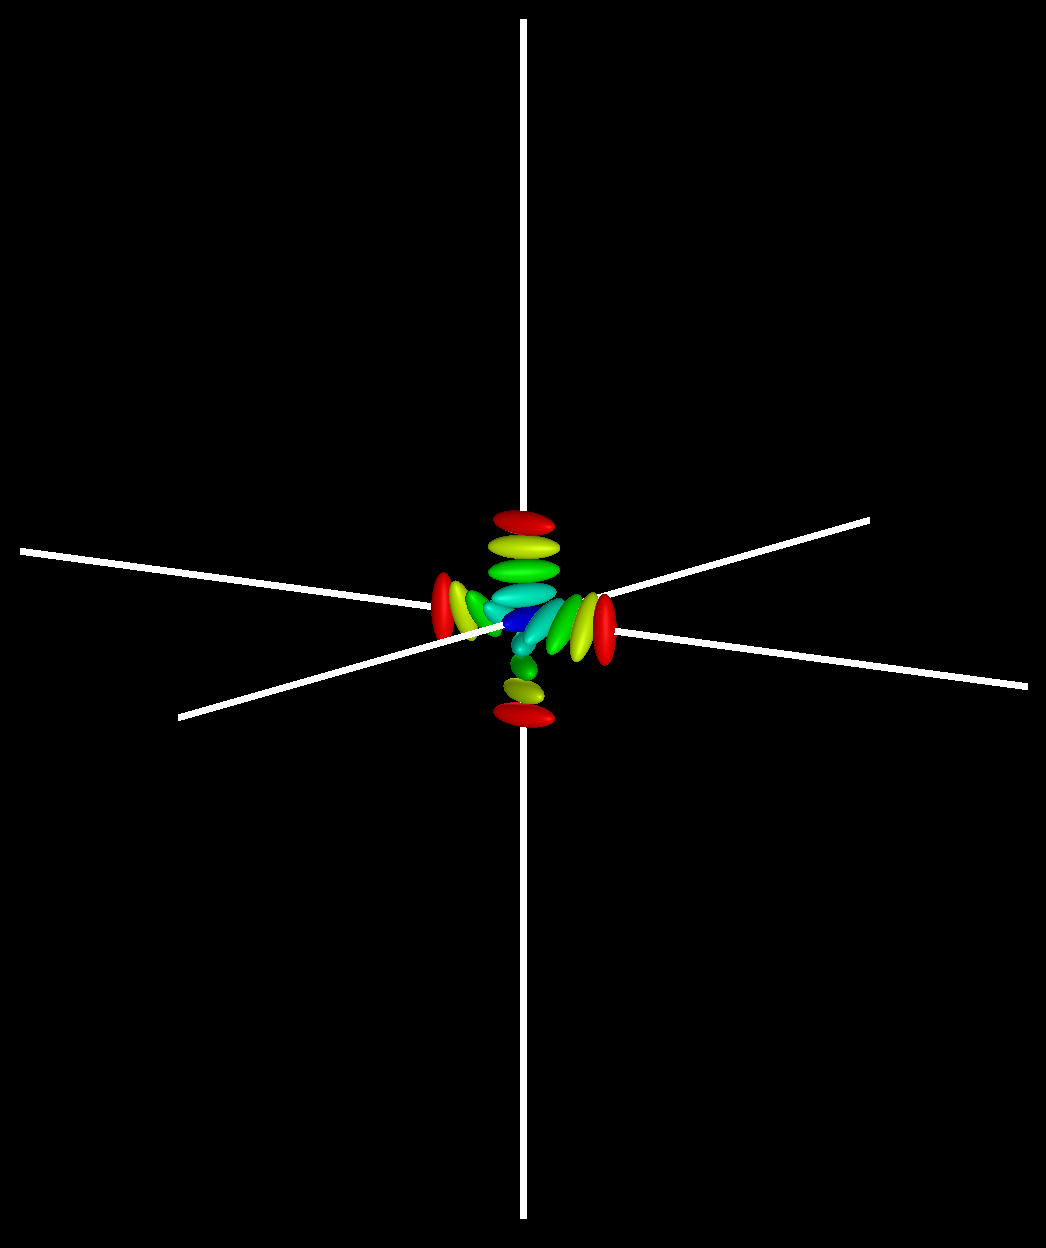
\includegraphics[width=\linewidth]{assets/images/axes/2_no_colour}
      \caption{Colour disabled}
      \label{fig:original_axes_no_colour}
    \end{subfigure}
    \begin{subfigure}{0.4\textwidth}
      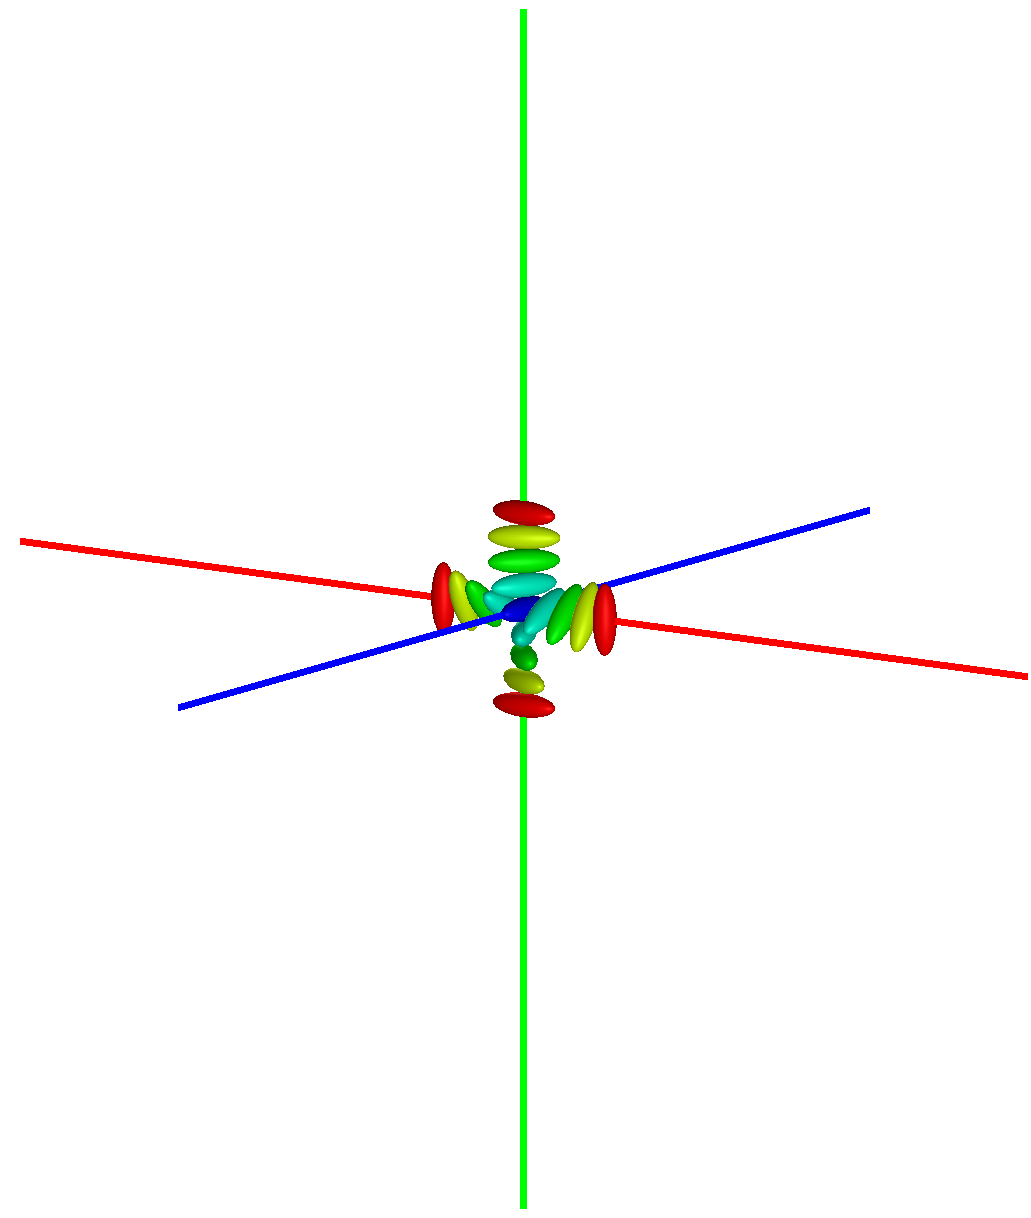
\includegraphics[width=\linewidth]{assets/images/axes/2_colour}
      \caption{Colour enabled}
      \label{fig:original_axes_colour}
    \end{subfigure}
    \begin{subfigure}{0.4\textwidth}
      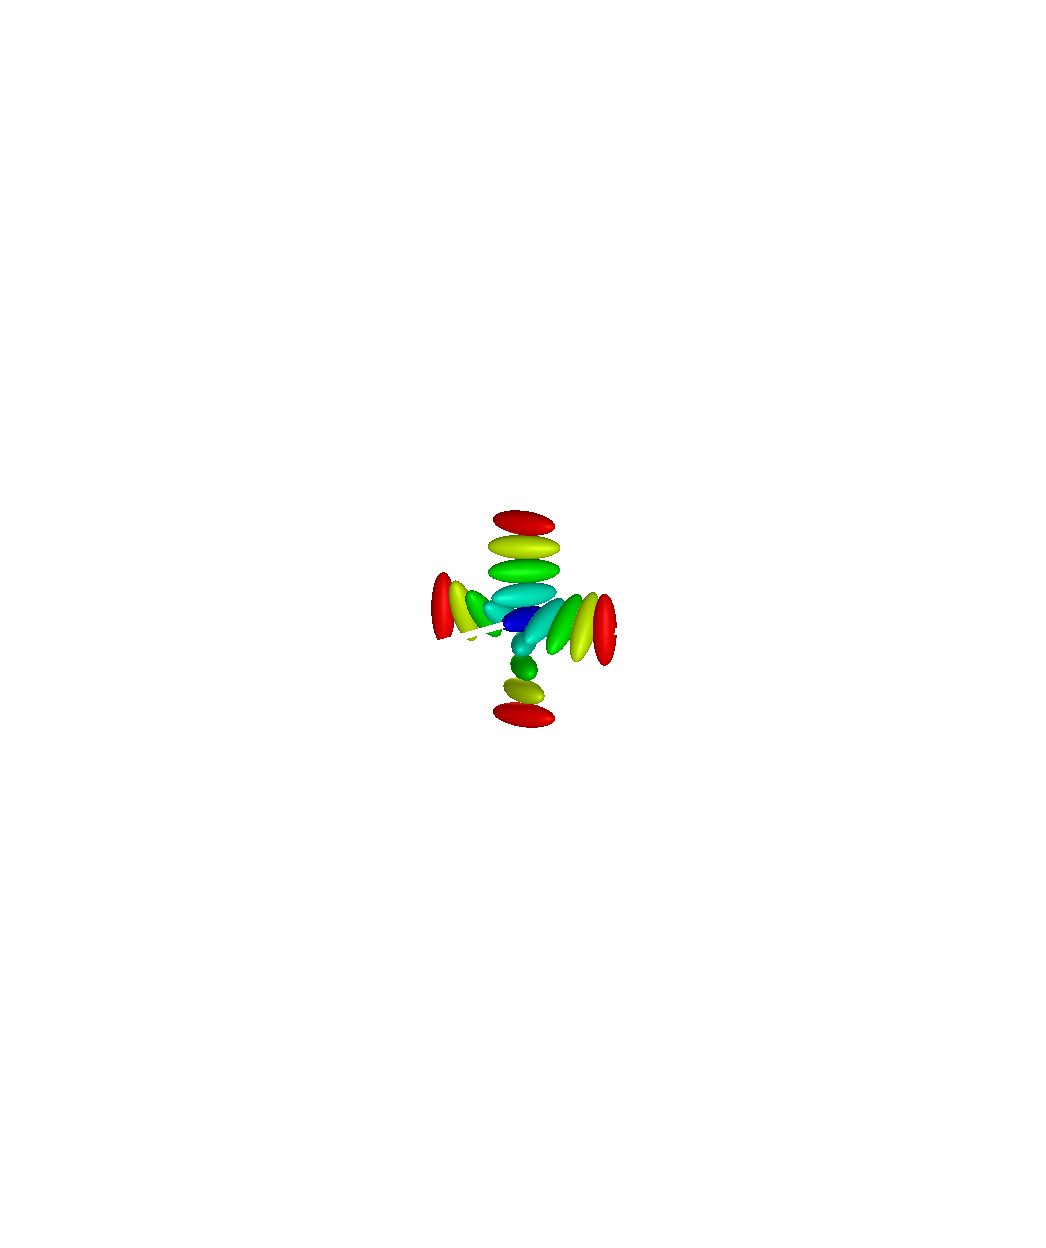
\includegraphics[width=\linewidth]{assets/images/axes/2_no_colour_bad}
      \caption{Colour disabled (light background)}
      \label{fig:original_axes_no_colour_bad}
    \end{subfigure}
    \begin{subfigure}{0.4\textwidth}
      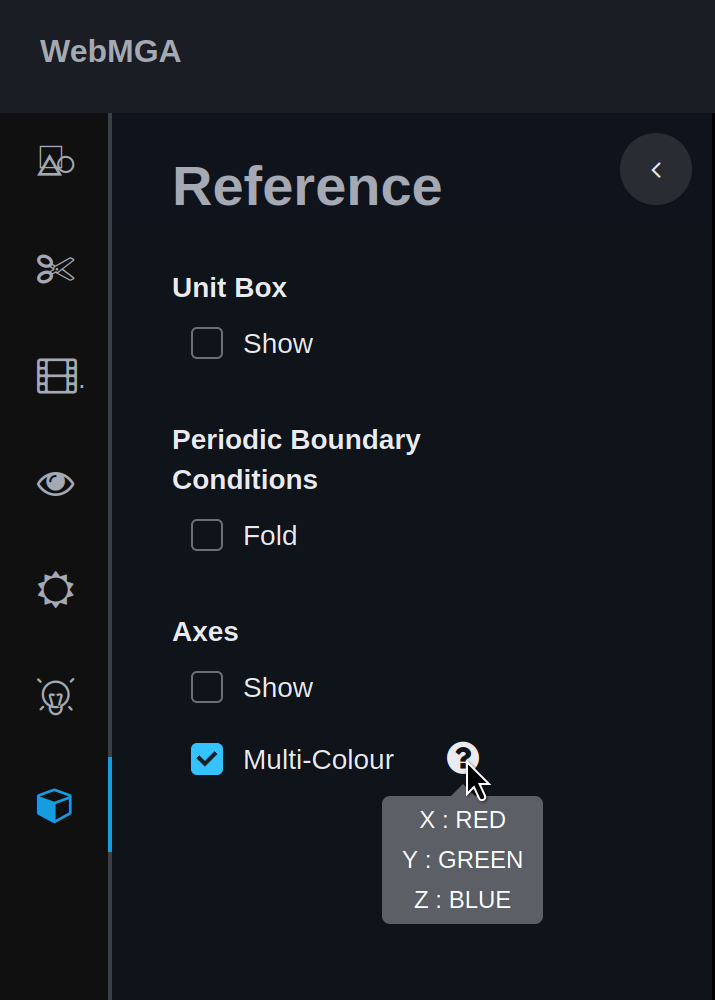
\includegraphics[width=\linewidth]{assets/images/axes/2_gui}
      \caption{GUI controls}
      \label{fig:original_axes_controls}
    \end{subfigure} 
  \end{center}
  \caption{Axes in WebMGA 2.0}
  \label{fig:original_axes}
\end{figure}

In WebMGA 2.0, the 3D axes are displayed as shown in \cref{fig:original_axes_no_colour,fig:original_axes_colour}, and controlled through the user interface as shown in \cref{fig:original_axes_controls} (visibility and colour toggles).

Axes take the form of three lines of fixed lengths in the $x$, $y$, and $z$ directions. Each line's midpoint is the lab fram coordinate $(0, 0, 0)$, where all axes meet. Axes extend in both positive and negative directions. They are not shown by default and, when first enabled, are uncoloured. When coloured, the $x$ axis is red, the $y$ axis is green, and the $z$ axis is blue.

Visibility is toggled using the ``Show'' button and colour is toggled with the ``Multi-Colour'' button. A question mark icon is next to the ``Multi-Colour'' which shows a tooltip when hovered specifying the axis colour scheme.

\subsection{WebMGA 2.0 Bugs}
\begin{figure}
  \begin{center}
    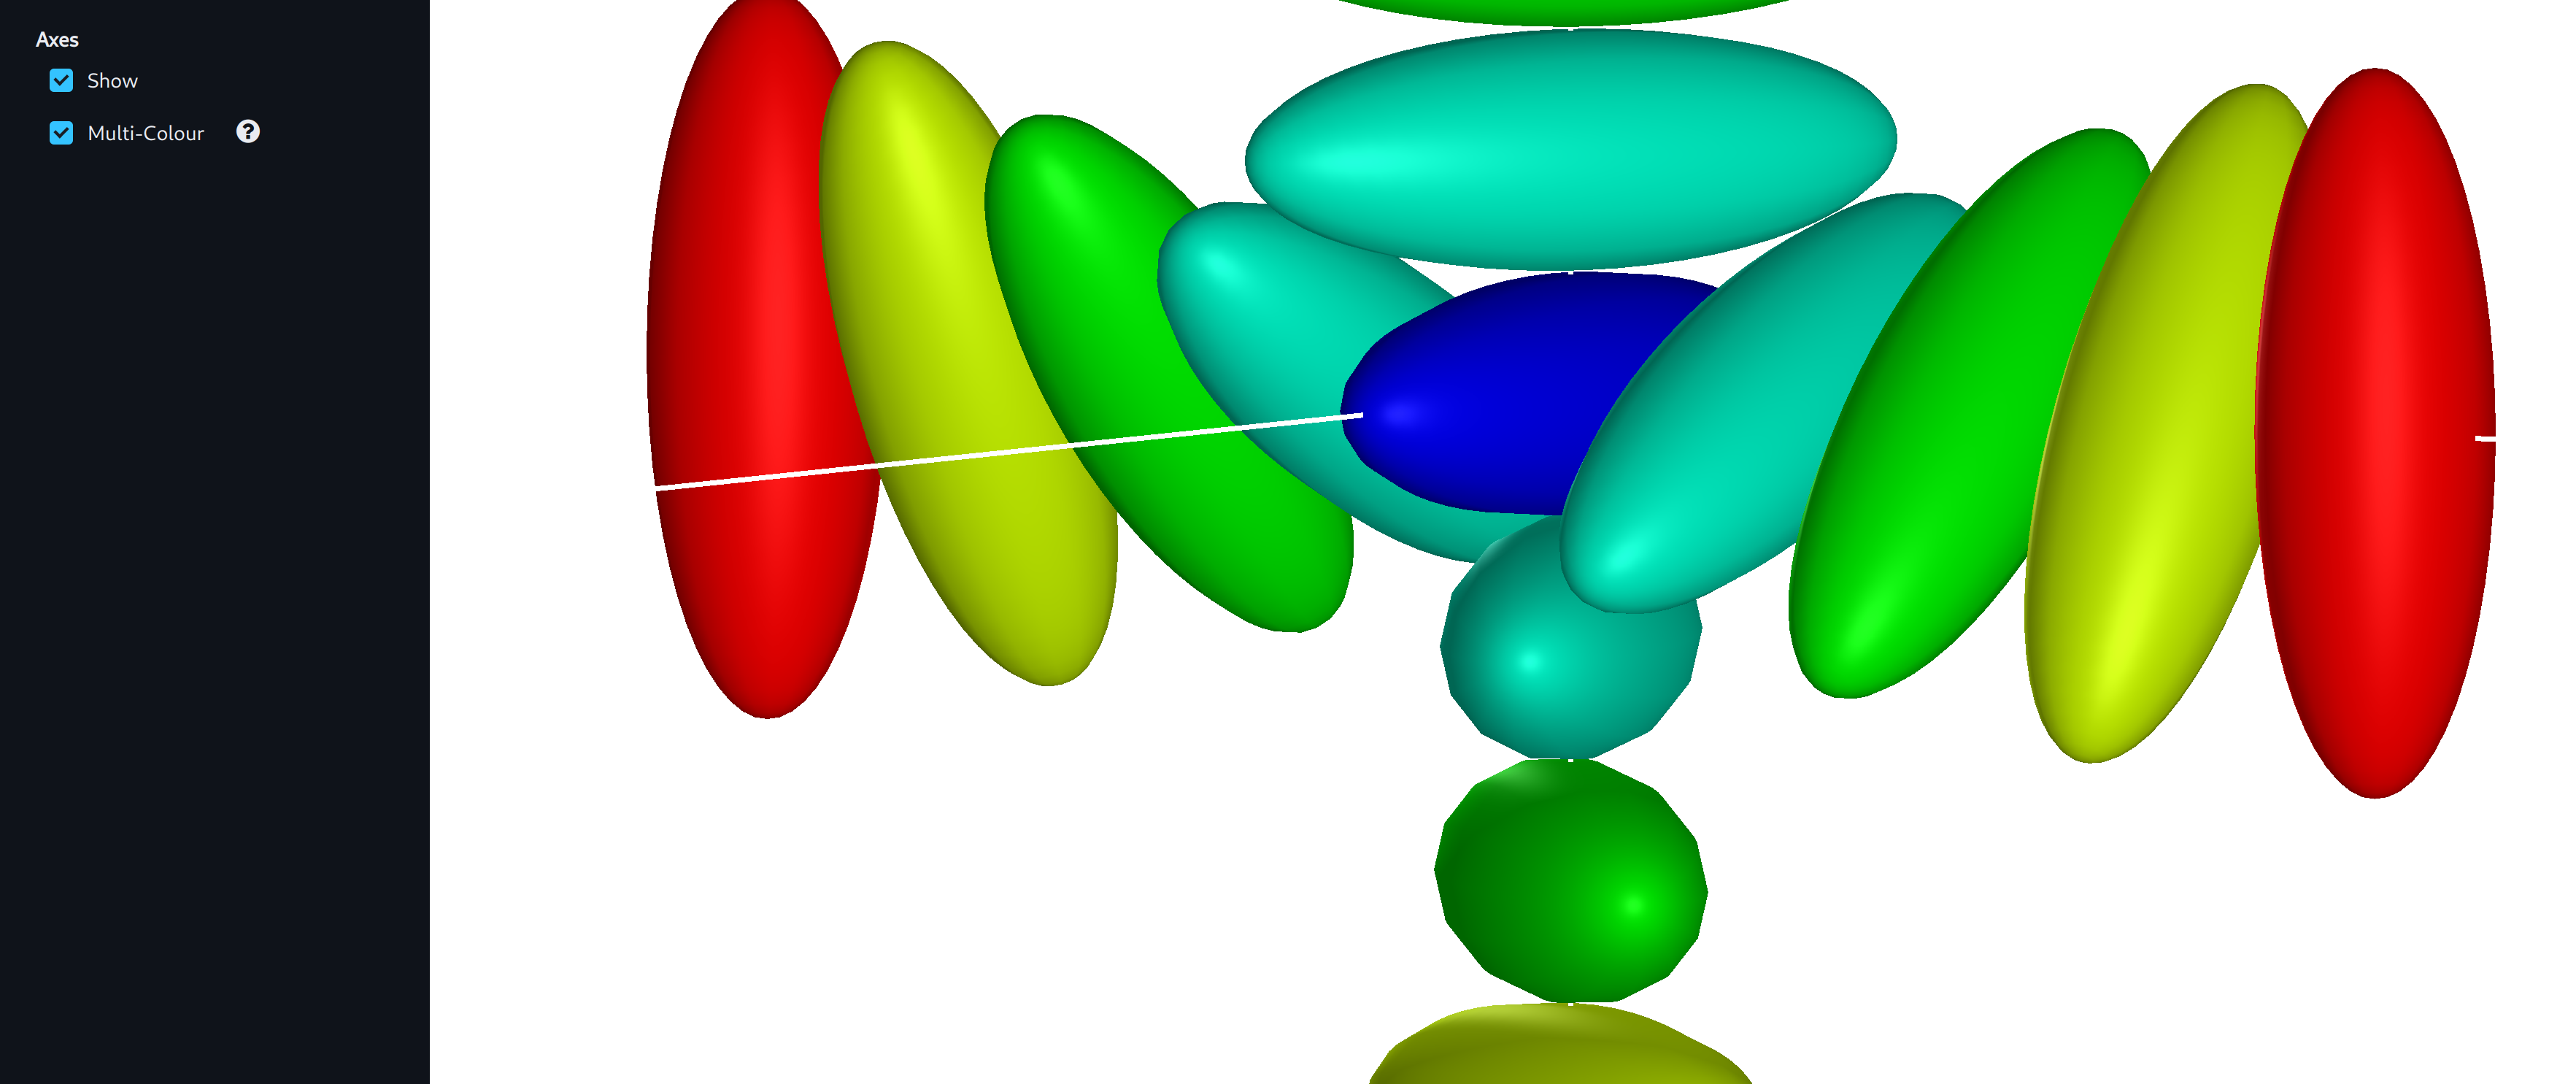
\includegraphics[width=\linewidth]{assets/images/axes/2_bug}
    \caption{\centering Bug where axes are not coloured despite the ``Multi-Colour'' toggle being enabled when axes are first enabled.}
    \label{fig:original_bug}
  \end{center}
\end{figure}

When the axes are toggled to visible for the first time, if the ``Multi-Colour'' toggle has not been interacted with first, the axes will be uncoloured, despite the ``Multi-Colour'' toggle being enabled by default. This is shown in \cref{fig:original_bug}. To enable colour for the first time, the "Multi-Colour" toggle must be disabled and then re-enabled.

When the environment is set to light mode (white background) with coloured axes disabled, the axes become difficult to view since they retain a white colour as default, blending into the background as shown in \cref{fig:original_axes_no_colour_bad}.

\subsection{Improvement Goals}
\begin{itemize}
  \item Axes are unlabelled
    \begin{itemize}
      \item Axes should be changed to extend only in the positive direction
    \end{itemize}
  \item Director(TODO label) is not shown
    \begin{itemize}
      \item An additional line should be shown indicating director direction
    \end{itemize}
  \item Colours should be labelled or meaningful
    \begin{itemize}
      \item Colour axes according to angle with director (as in TODO REFERENCE)
    \end{itemize}
  \item Axes should not be obscured
    \begin{itemize}
      \item Place axes in screen corner rather than centre
    \end{itemize}
  \item Axes should be clearly distinguishable
    \begin{itemize}
      \item Ensure axes retain contrast with background under light and dark views
    \end{itemize}
\end{itemize}

\subsection{WebMGA 3.0 Implementation}
\subsubsection{Axes Positions}
The existing implementation was found to be needlessly convoluted so was largely stripped out. For example, coloured and uncoloured axes were implemented entirely separately, resulting in a large amount of duplicated code and convoluted logic flow. The bug identified in WebMGA 2.0 regarding uncoloured axes showing with "Multi-Colour" enabled, for example, was found to occur due to incorrect colour object initialisation, meaning what should be "Multi-Colour" axes showed as uncoloured since the colours are not defined when these lines are loaded the very first time.

In the new axes code, they are simply defined in terms of an axes centre point, three axes vectors, and an axis length scale. The axes vectors are handled in the lab frame so are trivially defines as $x=(1,0,0)$, $y=(0,1,0)$, and $z=(0,0,1)$.

Since the axes centre needs to remain in a fixed position on screen at all times, it needs to be defined relative to the camera. Three.js provides a method on any world object which converts from object relative coordinates to the lab frame, so this is used to trivially place the axes centre into the lab fram as required. Since this relationship changes when an object, in this case the camera, moves, the axes centre must therefore be redefined on any camera movement. This process also does not account for changes to intrinsic camera properties, importantly camera zoom. The axes therefore need to be scaled proportionally to the camera's zoom level on any zoom change.

Using the lab frame centre point and the axes vectors and scales, axis lines are trivially defined as,

\begin{equation}
  l_0=c\label{axes_vector_1}
\end{equation}
\begin{equation}
  l_1=c+szv\label{axes_vector_2}
\end{equation}
where $l_0$ and $l_1$ are the axis line start and end, $c$ is the axes centre, $v$ is the axis vector, $s$ is the axis scale factor, and $z$ is the zoom factor of the camera. These can be recalculated and applied on every camera change. A Three.js Line object is constructed for each axis using the line start, end, and a colour.

\subsubsection{Director}
Plotting the director is made simple using the above setup. A new axis is simply defined using \cref{axes_vector_1,axes_vector_2}, with $v$ set to the already computed director vector (TODO show where this was done).

\subsubsection{Axes Colouring}
It was decided that a meaningful colouring for the axes lines (including the director) would be using the same colour scheme as for molecule colour (TODO show where). This can be done easily since all axes have a defined direction vector which can be passed to the TODO COLOURFROMDIRECTORNAME function (TODO show where). The resulting colour is simply passed as part of the Line object constructor.

\subsubsection{Axes Summary}
\begin{figure}
  \begin{center}
    \begin{subfigure}{0.4\textwidth}
      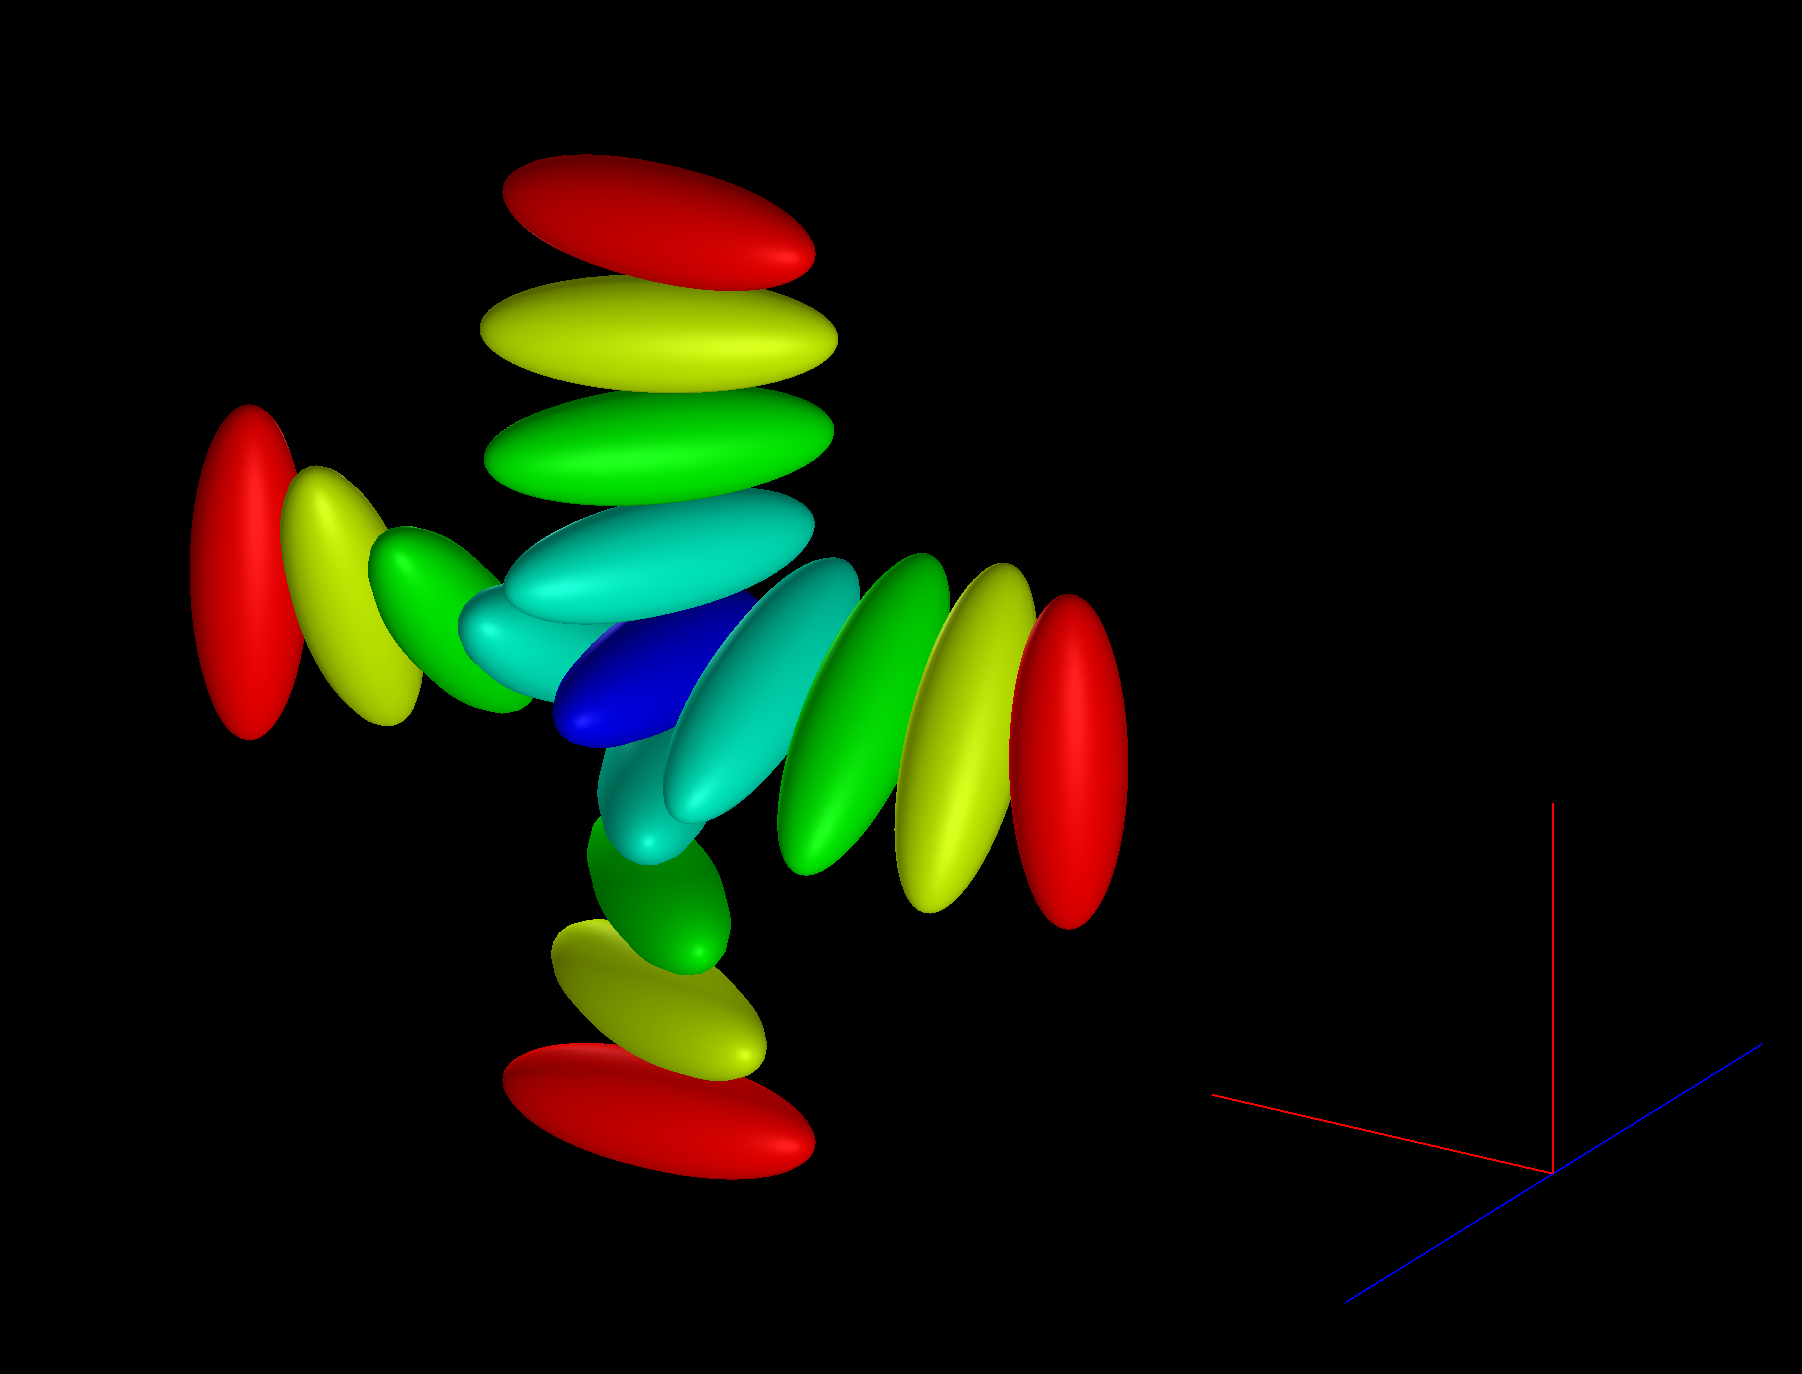
\includegraphics[width=\linewidth]{assets/images/axes/2_new_1}
      \caption{}
      \label{fig:2_new_1}
    \end{subfigure}
    \begin{subfigure}{0.4\textwidth}
      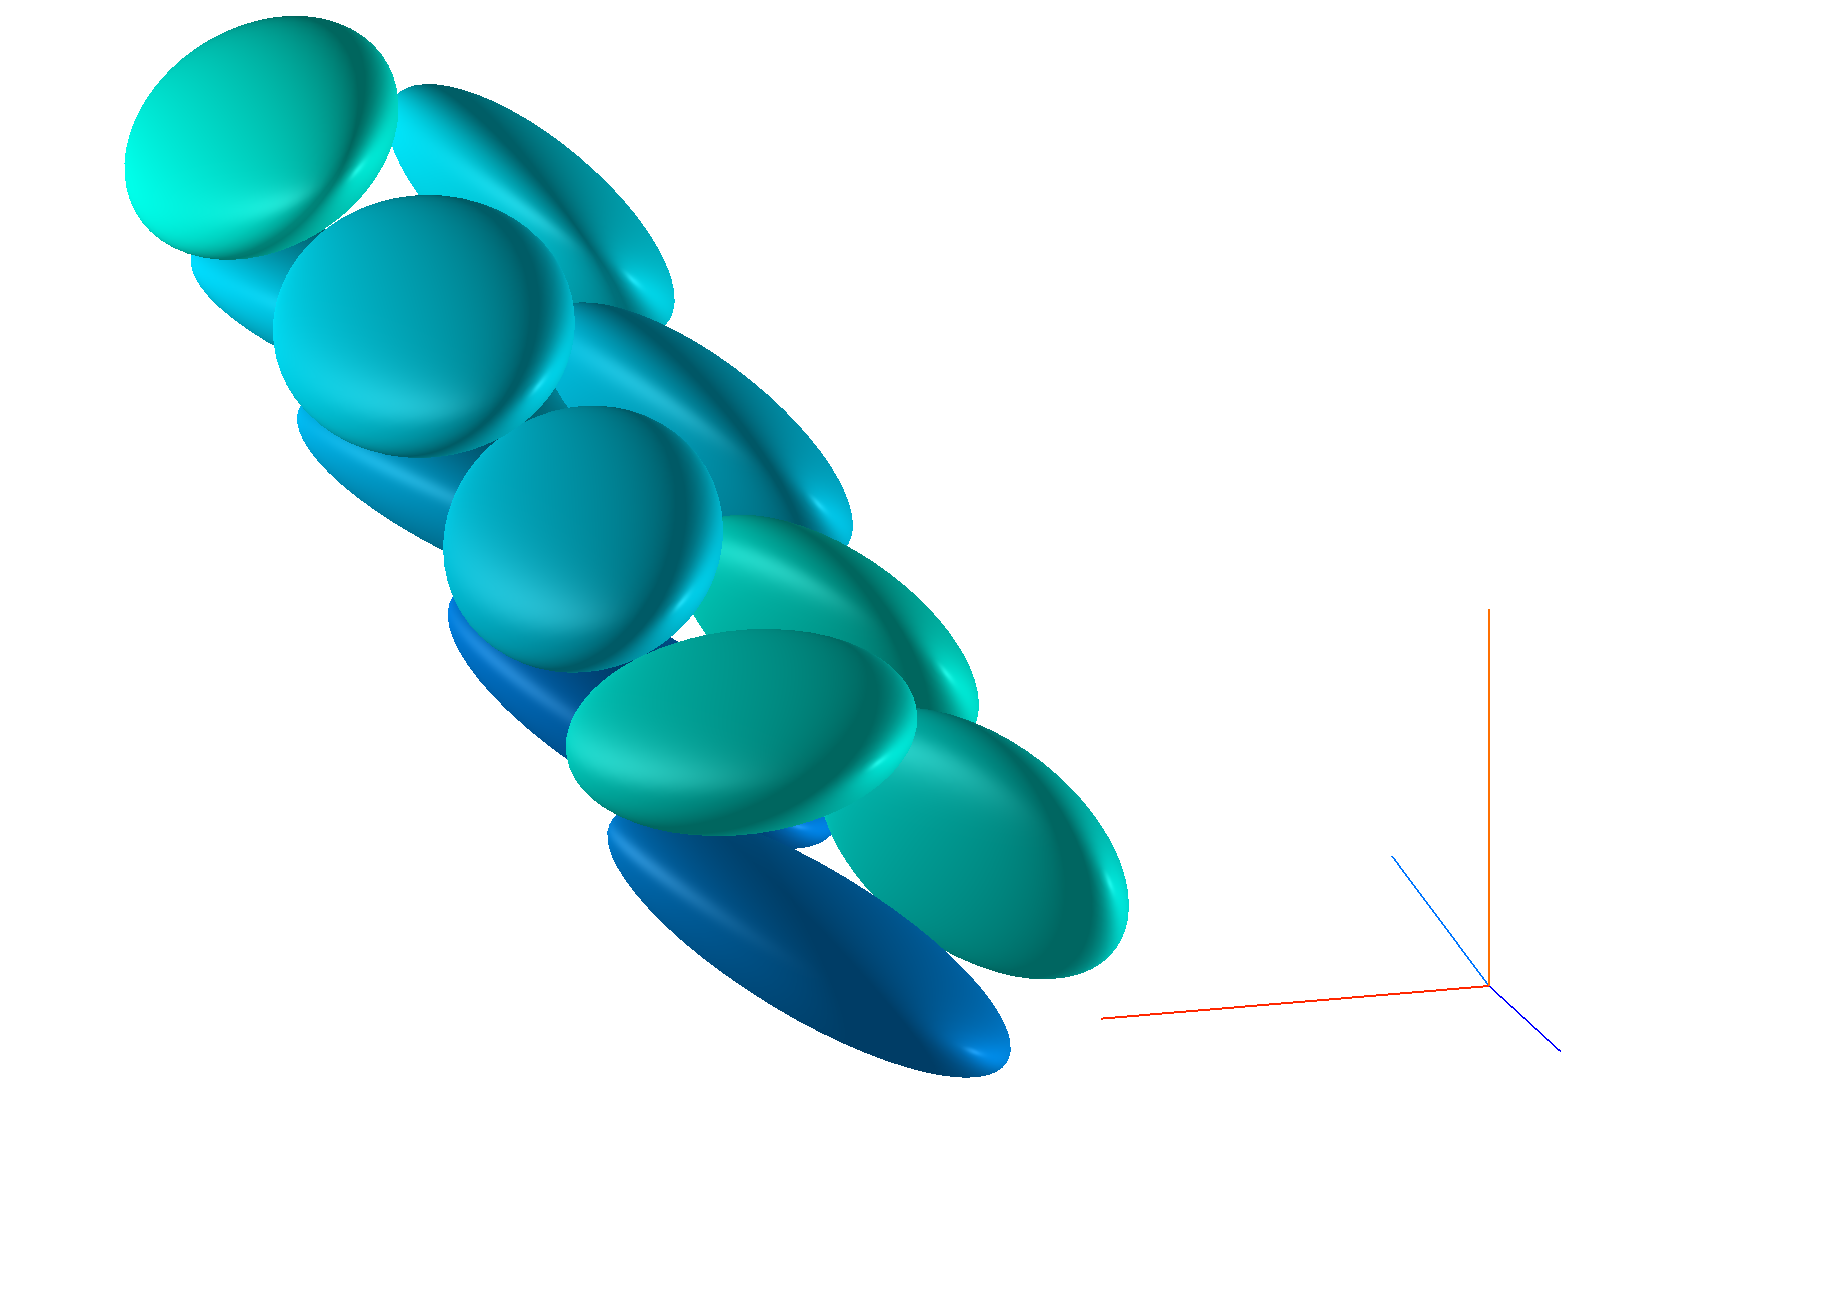
\includegraphics[width=\linewidth]{assets/images/axes/2_new_2}
      \caption{}
      \label{fig:2_new_2}
    \end{subfigure}
  \end{center}
  \caption{Axes in WebMGA 3.0}
  \label{fig:new_axes}
\end{figure}

Some result can be viewed in \cref{fig:new_axes}.

\subsubsection{GUI Implementation}
TODO discuss UI

\subsection{WebMGA 3.0 Bugs}
TODO

\newcommand{\shapefigurepartbase}[4]{
  \begin{subfigure}{0.2\textwidth}
    \includegraphics[width=\linewidth]{assets/images/shapes/#2/#1#3}
    \caption{\makefirstuc{#2 #4}}
    \label{fig:#2_#1#3}
  \end{subfigure}
}

\newcommand{\shapefigurepart}[2]{
  \shapefigurepartbase{#1}{#2}{}{model}
}

\newcommand{\shapefigurepartw}[2]{
  \shapefigurepartbase{#1}{#2}{_w}{wireframe}
}

\newcommand{\shapefigure}[2]{
\begin{figure}
  \begin{center}
    \shapefigurepart{#1}{old}
    \shapefigurepartw{#1}{old}
    \shapefigurepart{#1}{new}
    \shapefigurepartw{#1}{new}
  \end{center}
  \caption{\makefirstuc{#2 molecule mesh implementation.}}
  \label{fig:#1_shape}
\end{figure}
}

\newcommand{\oldshapefigure}[1]{
\begin{figure}
  \begin{center}
    \shapefigurepart{#1}{old}
    \shapefigurepartw{#1}{old}
  \end{center}
  \caption{\makefirstuc{#1}}
  \label{fig:#1_shape}
\end{figure}
}

\newcommand{\newshapefigure}[2]{
\begin{figure}
  \begin{center}
    \shapefigurepart{#1}{new}
    \shapefigurepartw{#1}{new}
  \end{center}
  \caption{\makefirstuc{#2}}
  \label{fig:#1_shape}
\end{figure}
}

\section{Shapes}
\label{shapes_section}
\subsection{WebMGA 2.0 Implementation}
WebMGA 2.0 implements the following molecule shapes:
\begin{itemize}
  \item Sphere (\cref{fig:sphere_shape})
  \item Ellipsoid (\cref{fig:ellipsoid_shape})
  \item Spherocylinder (\cref{fig:spherocylinder_shape})
  \item Spheroplatelet (\cref{fig:spheroplatelet_shape})
  \item Cut Sphere (\cref{fig:doublecutsphere_shape}, implemented as a double cut sphere)
  \item Cylinder (\cref{fig:cylinder_shape})
  \item Torus (\cref{fig:torus_shape})
\end{itemize}
Notably missing but useful are the single cut sphere, the spherical cap, and the lens. The cylinder and torus shapes are present since the three.js library provides easily callable predefined meshes, however serve little practical purpose since no realistic molecular configuration would model using these.
\oldshapefigure{cylinder}
\oldshapefigure{torus}

\subsection{WebMGA 2.0 Bugs}
\begin{figure}
  \begin{center}
    \begin{subfigure}{0.2\textwidth}
    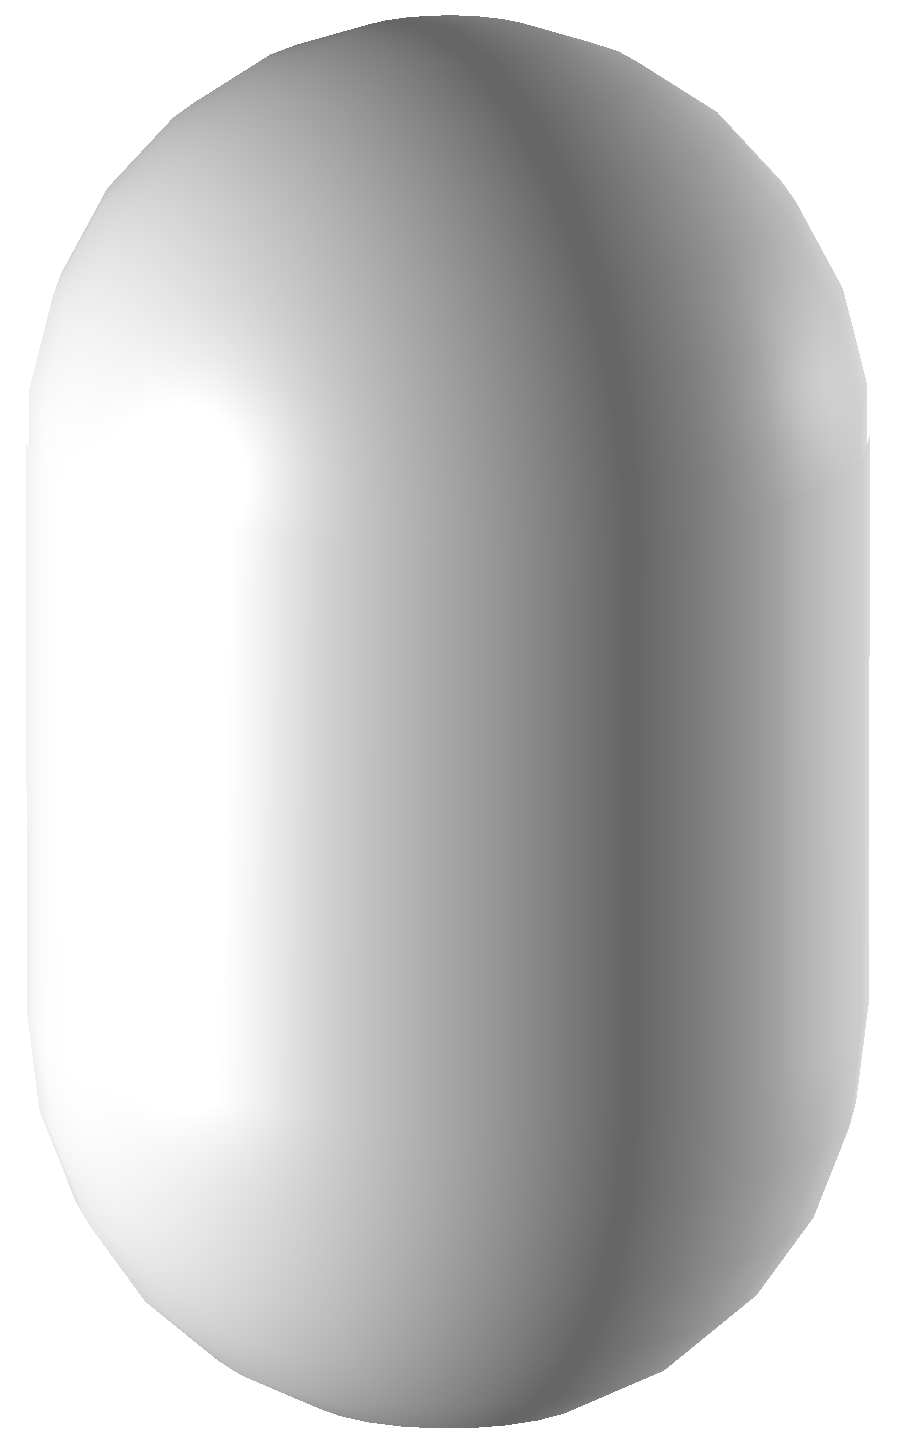
\includegraphics[width=\linewidth]{assets/images/shapes/bugold/bad_mesh_high}
    \caption{\makefirstuc{WebMGA 2.0 high detail shape}}
    \end{subfigure}
      \begin{subfigure}{0.2\textwidth}
    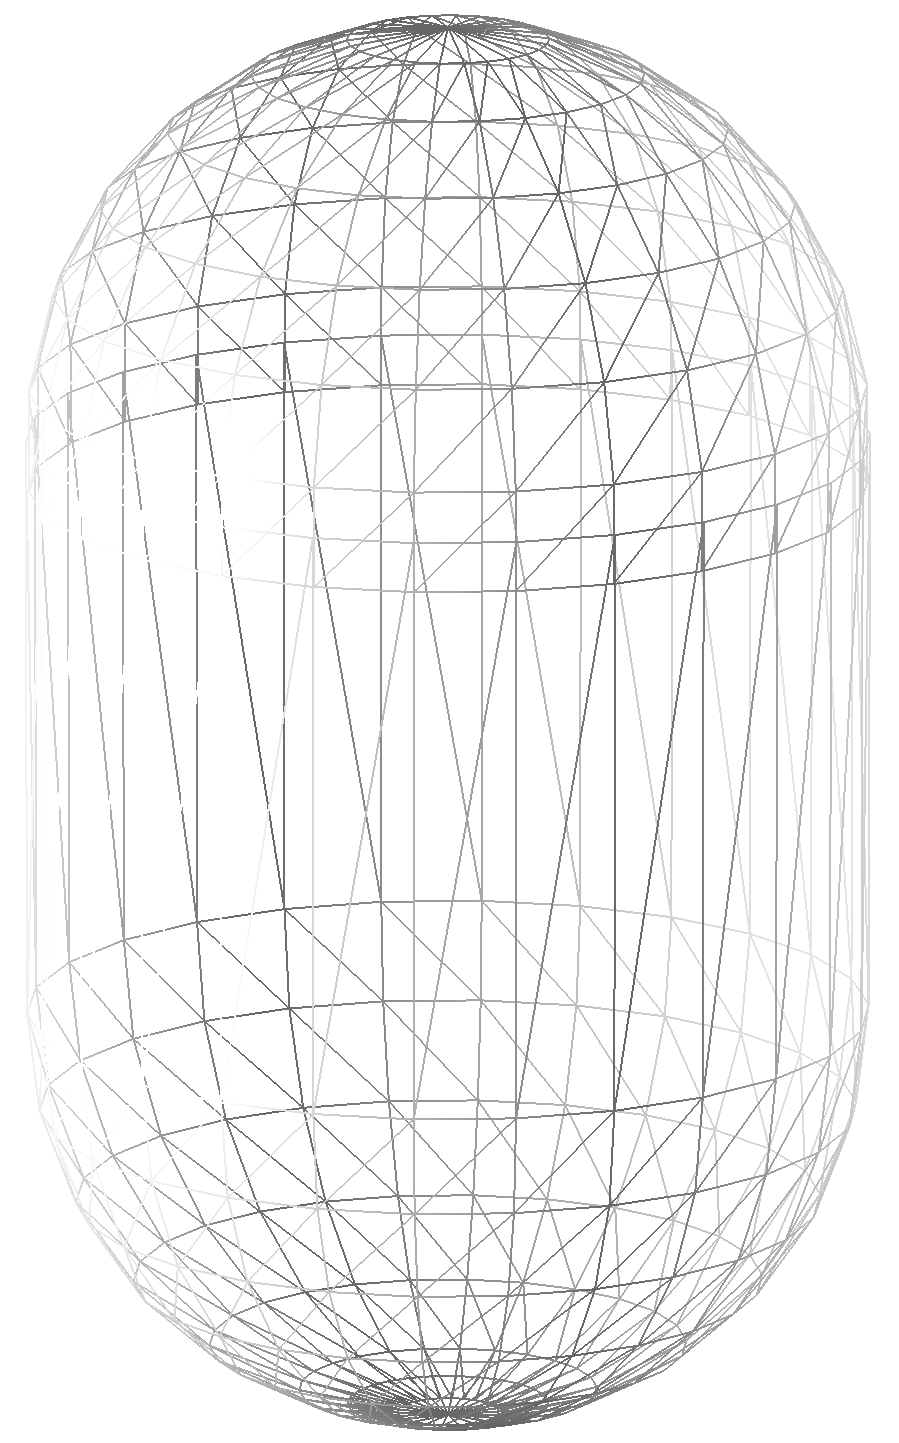
\includegraphics[width=\linewidth]{assets/images/shapes/bugold/bad_mesh_high_w}
    \caption{\makefirstuc{WebMGA 2.0 high detail mesh}}
    \end{subfigure}
    \begin{subfigure}{0.2\textwidth}
    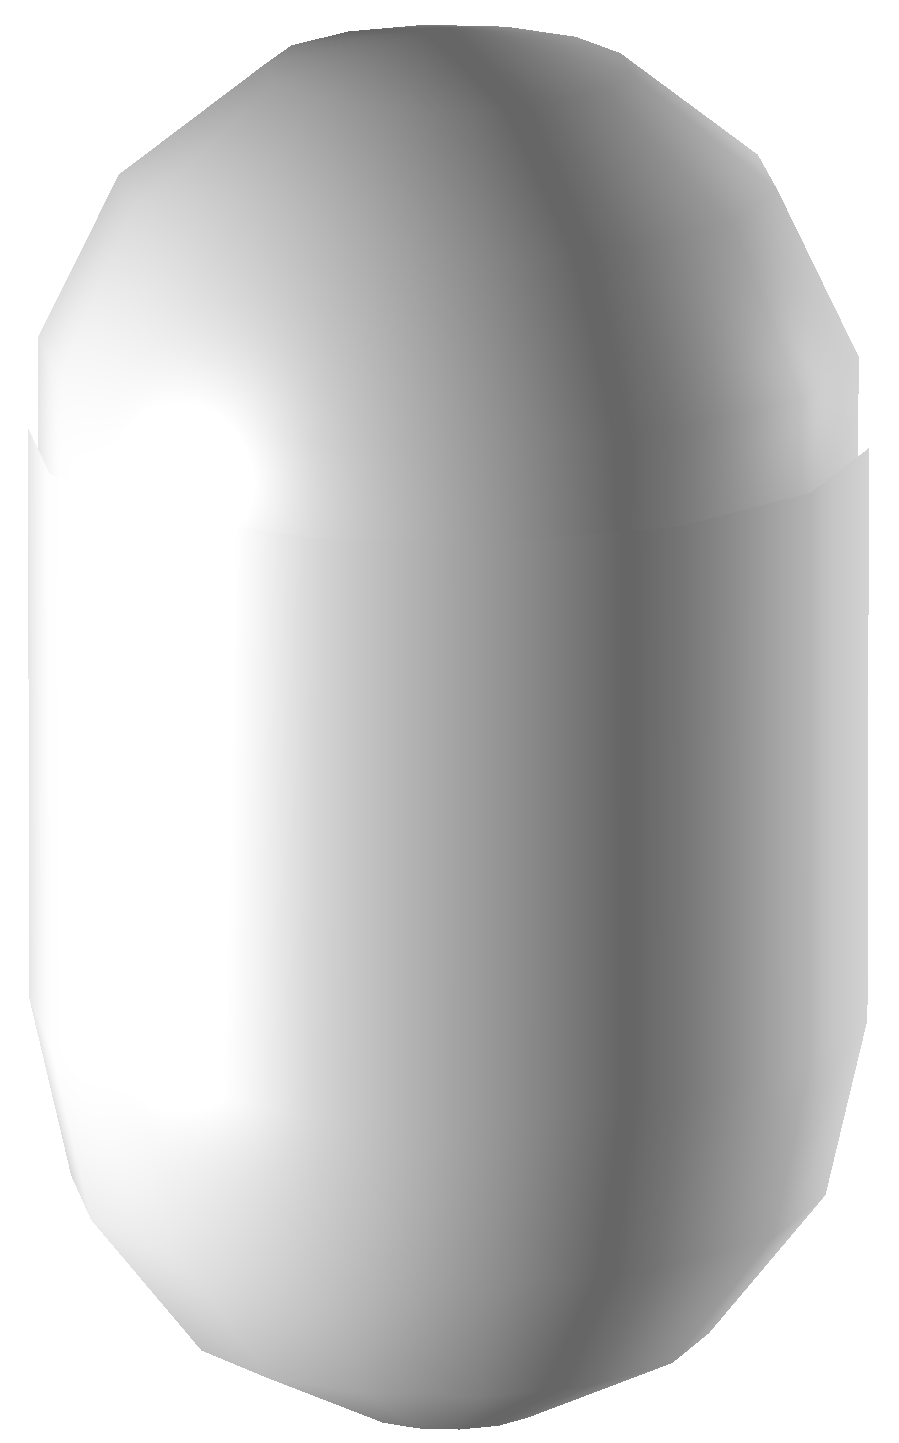
\includegraphics[width=\linewidth]{assets/images/shapes/bugold/bad_mesh_med}
    \caption{\makefirstuc{WebMGA 2.0 medium detail shape}}
    \end{subfigure}
    \begin{subfigure}{0.2\textwidth}
    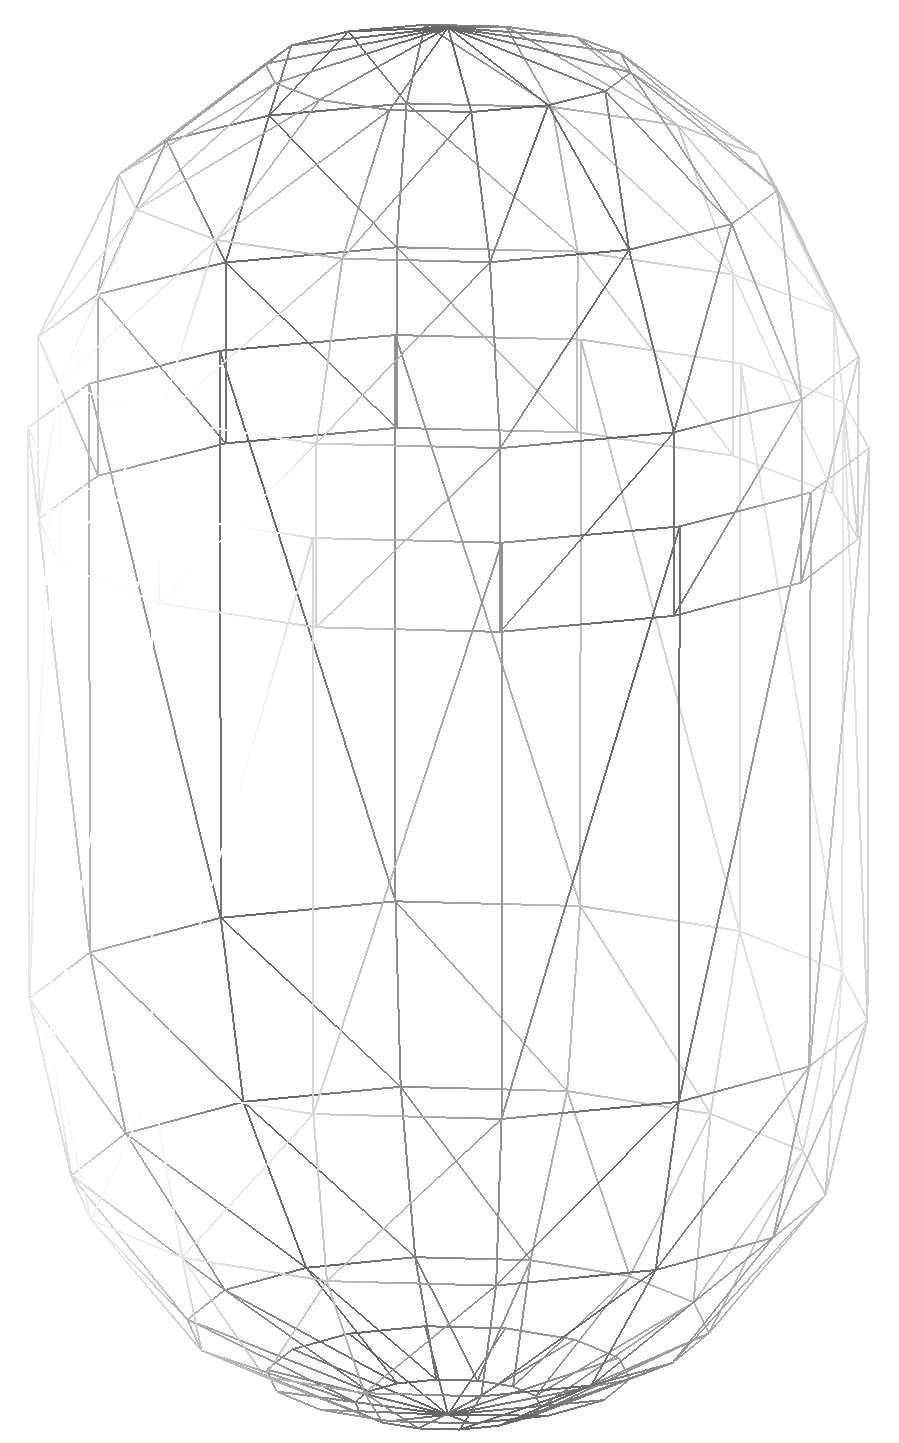
\includegraphics[width=\linewidth]{assets/images/shapes/bugold/bad_mesh_med_w}
    \caption{\makefirstuc{WebMGA 2.0 medium detail mesh}}
    \end{subfigure}
    \begin{subfigure}{0.2\textwidth}
    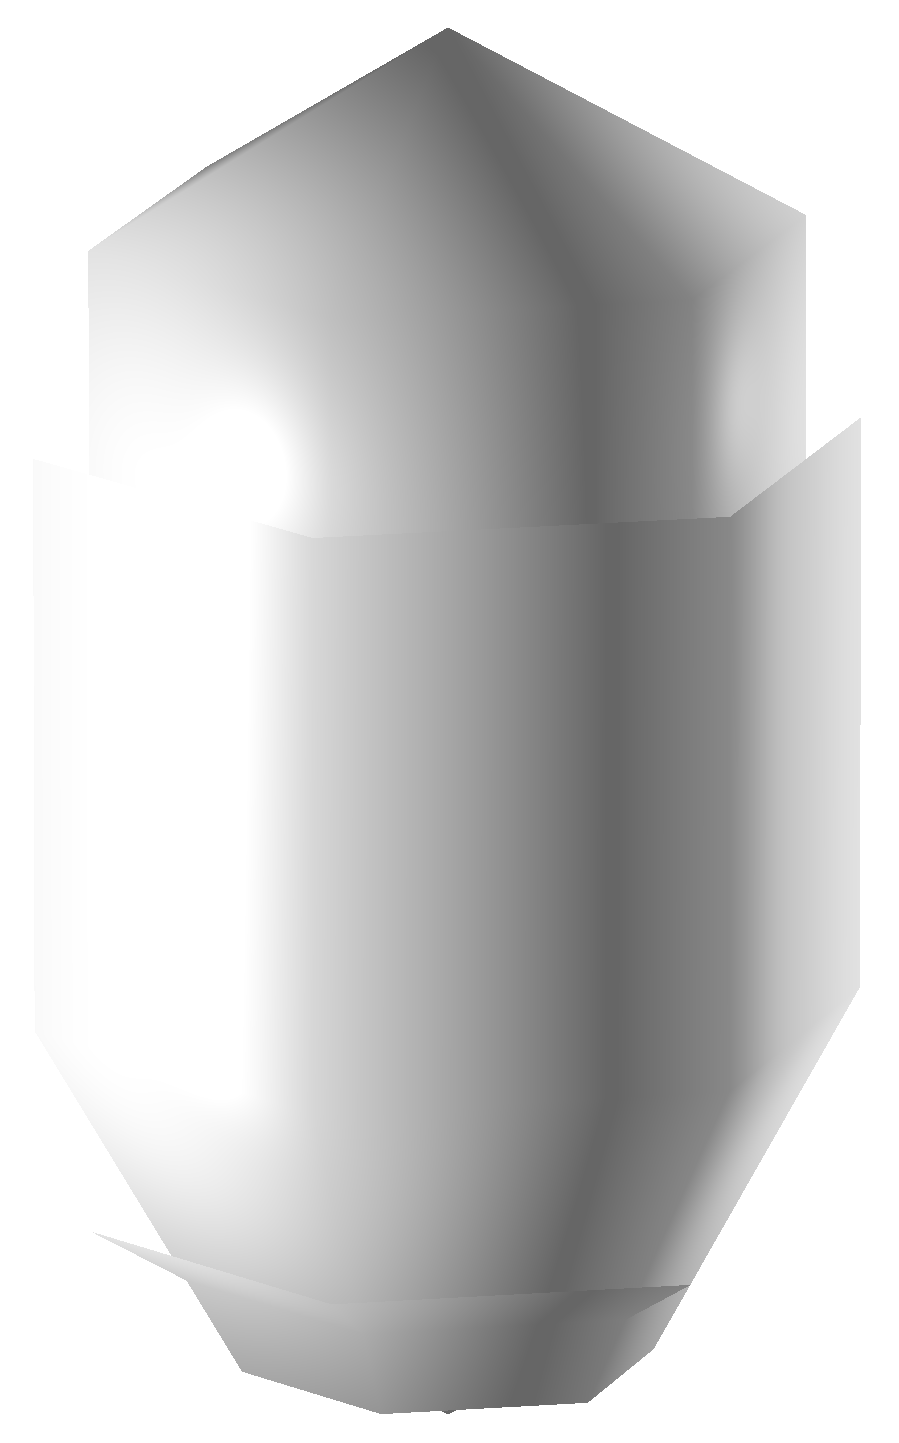
\includegraphics[width=\linewidth]{assets/images/shapes/bugold/bad_mesh_low}
    \caption{\makefirstuc{WebMGA 2.0 low detail shape}}
    \end{subfigure}
    \begin{subfigure}{0.2\textwidth}
    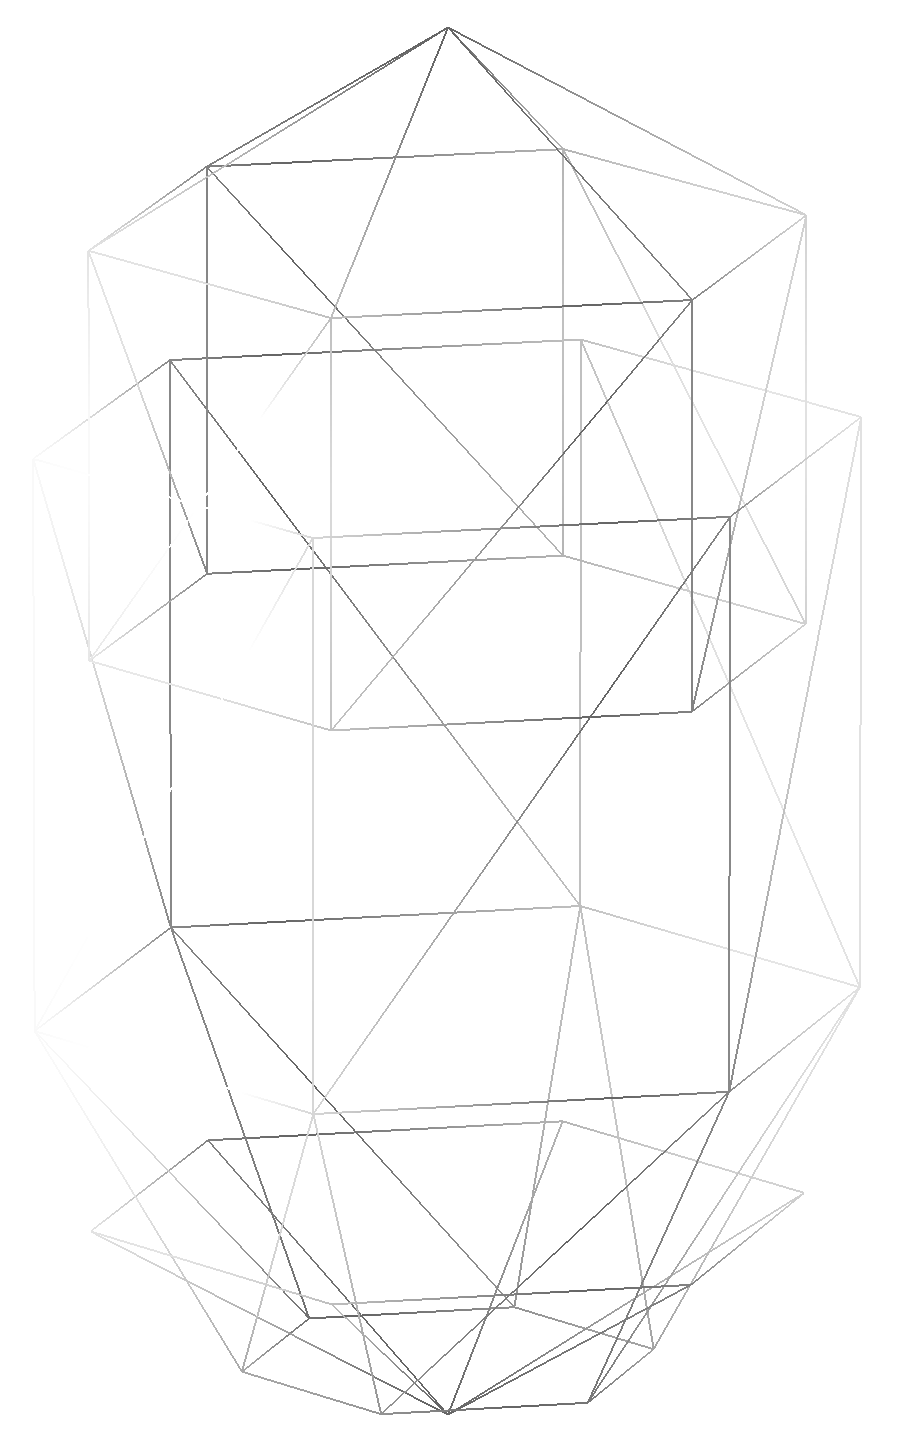
\includegraphics[width=\linewidth]{assets/images/shapes/bugold/bad_mesh_low_w}
    \caption{\makefirstuc{WebMGA 2.0 low detail mesh}}
    \end{subfigure}
  \end{center}
  \caption{\makefirstuc{Bad spheocylinder mesh generated by WebMGA 2.0}}
  \label{fig:bad_spherocylinder_old}
\end{figure}
\begin{figure}
  \begin{center}
    \begin{subfigure}{0.2\textwidth}
    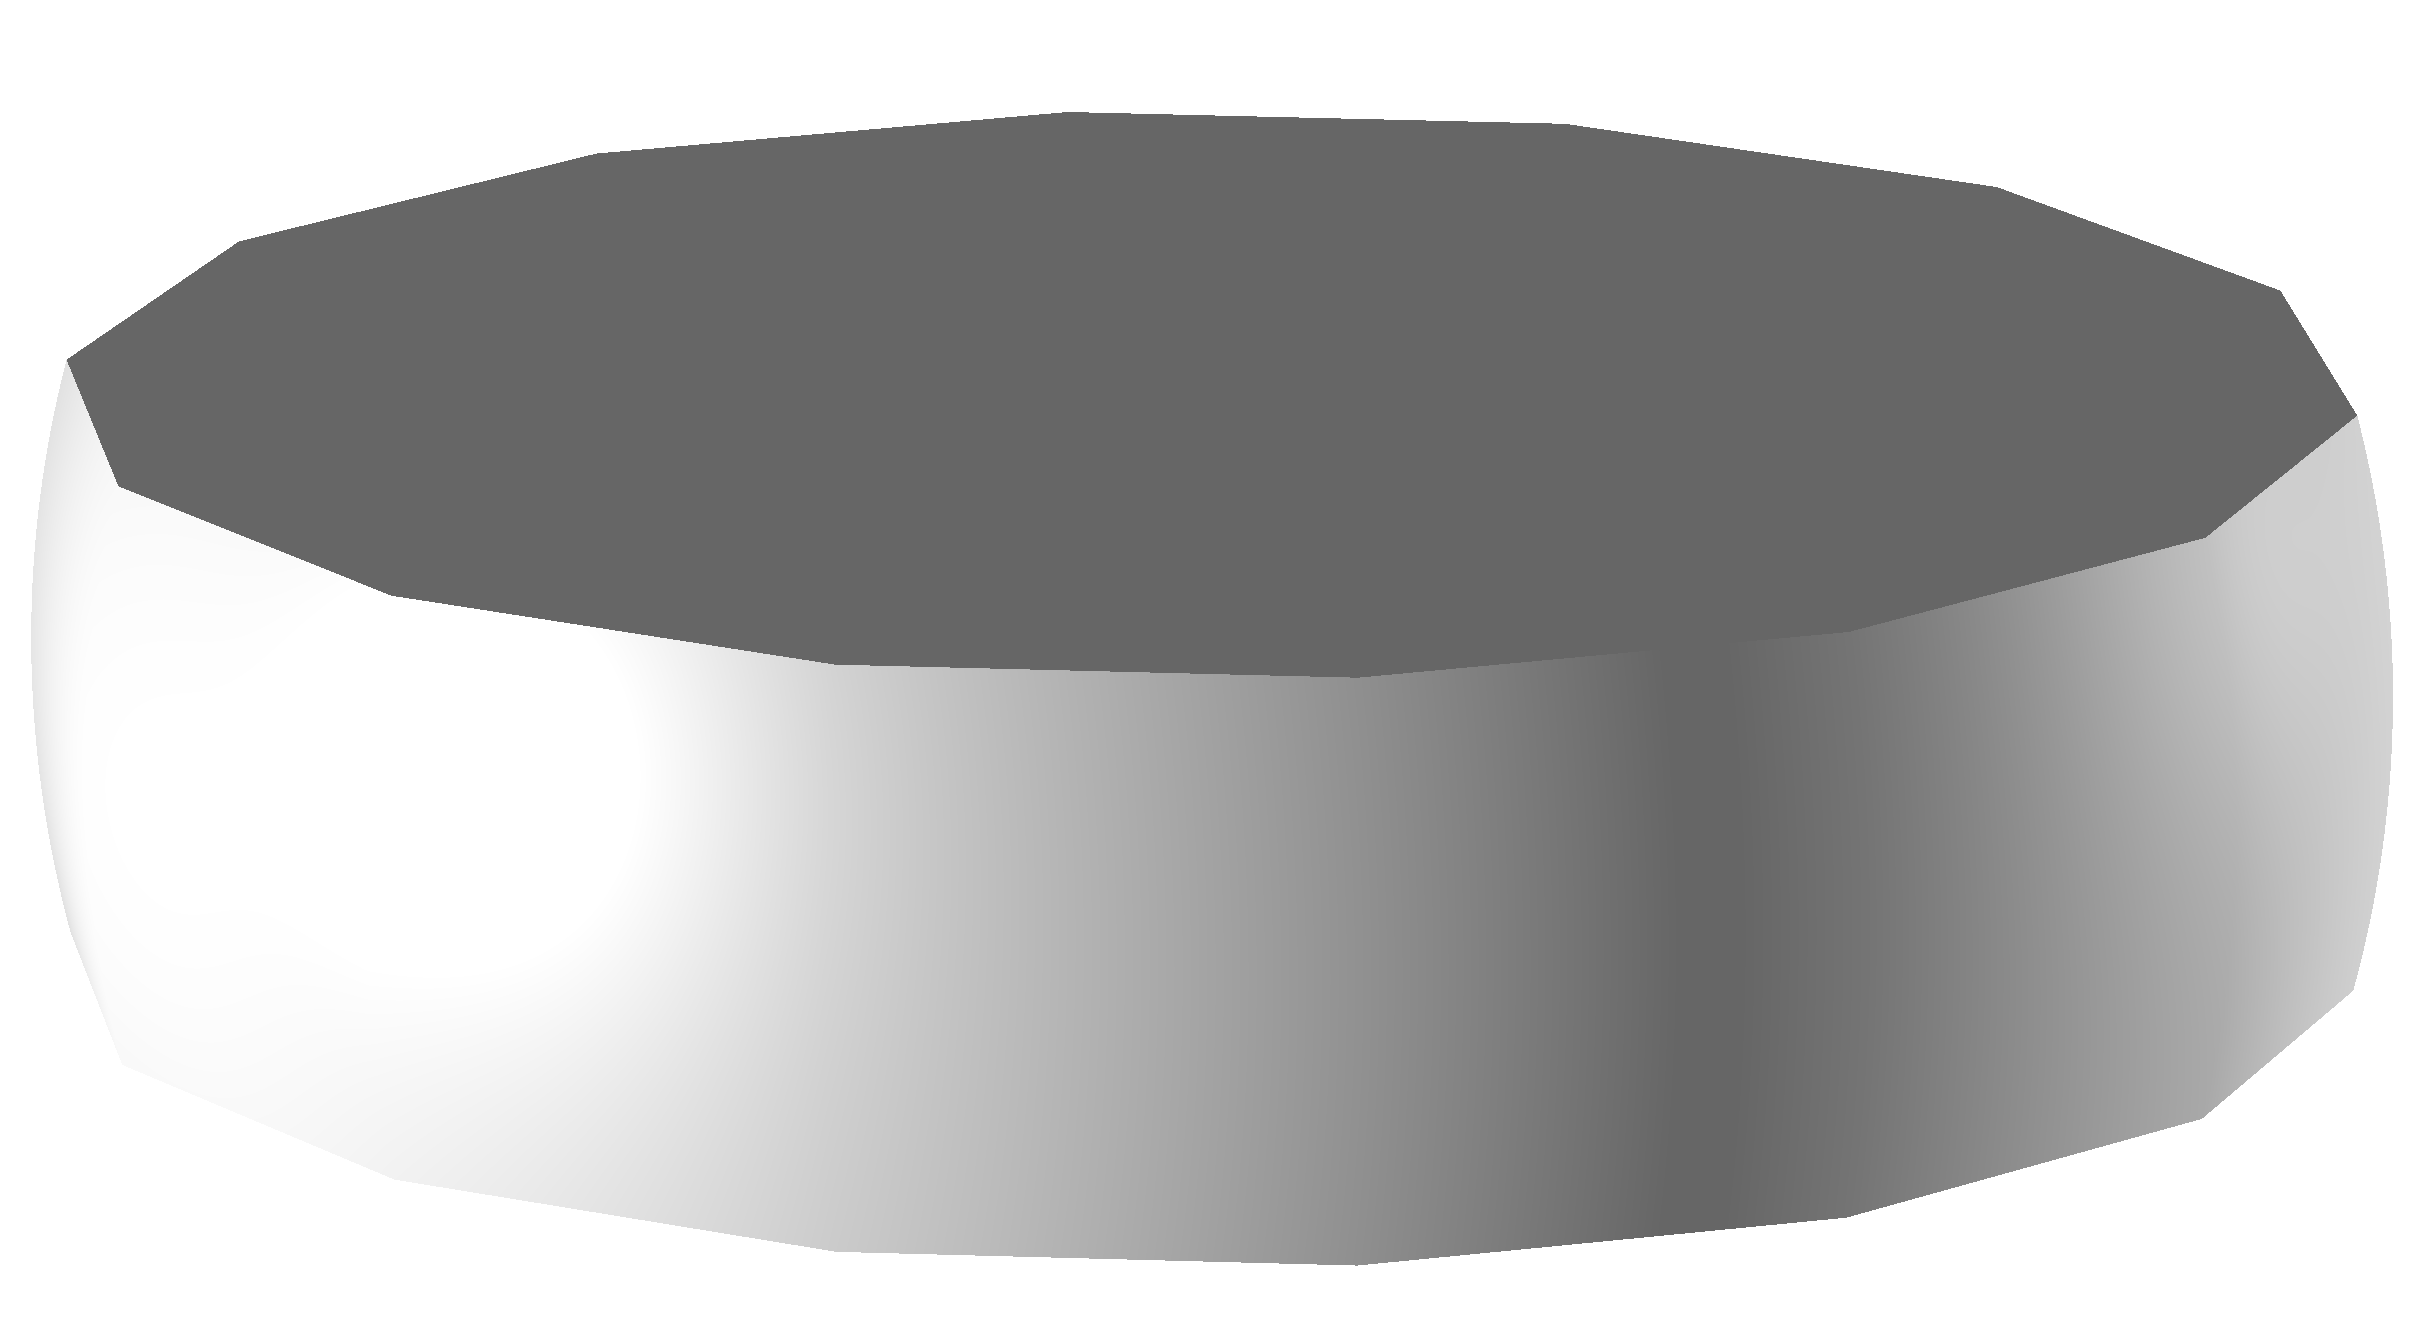
\includegraphics[width=\linewidth]{assets/images/shapes/bugold/scale_high}
    \caption{\makefirstuc{WebMGA 2.0}}
    \end{subfigure}
      \begin{subfigure}{0.2\textwidth}
    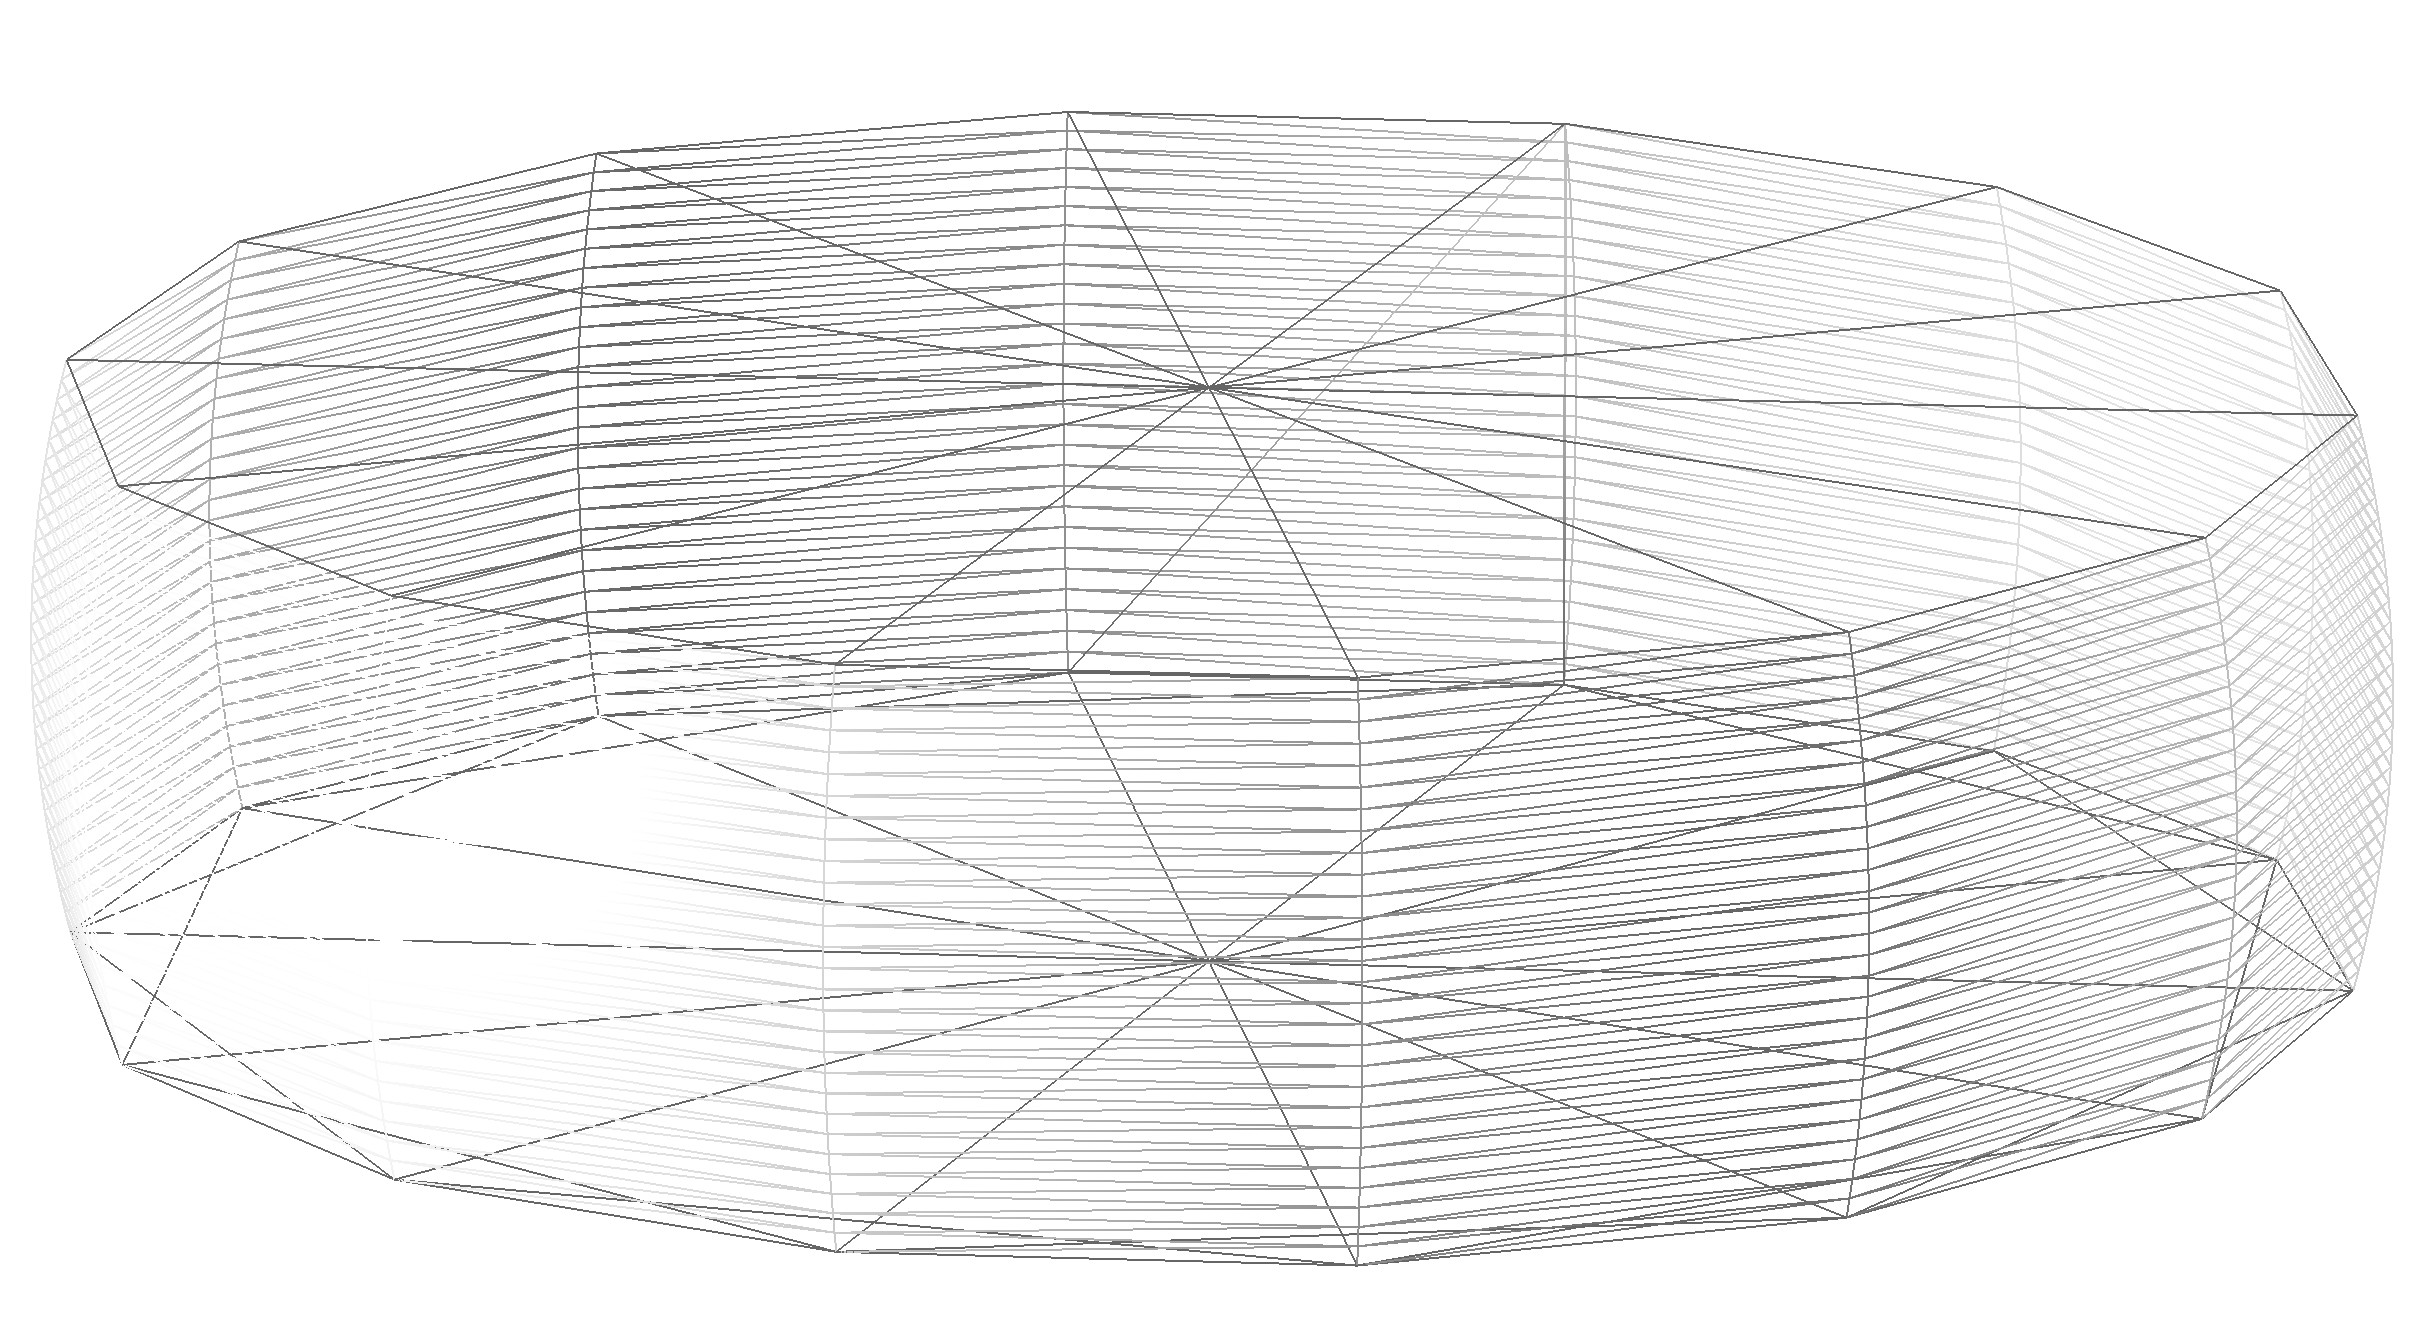
\includegraphics[width=\linewidth]{assets/images/shapes/bugold/scale_high_w}
    \caption{\makefirstuc{WebMGA 2.0}}
    \end{subfigure}
    \begin{subfigure}{0.2\textwidth}
    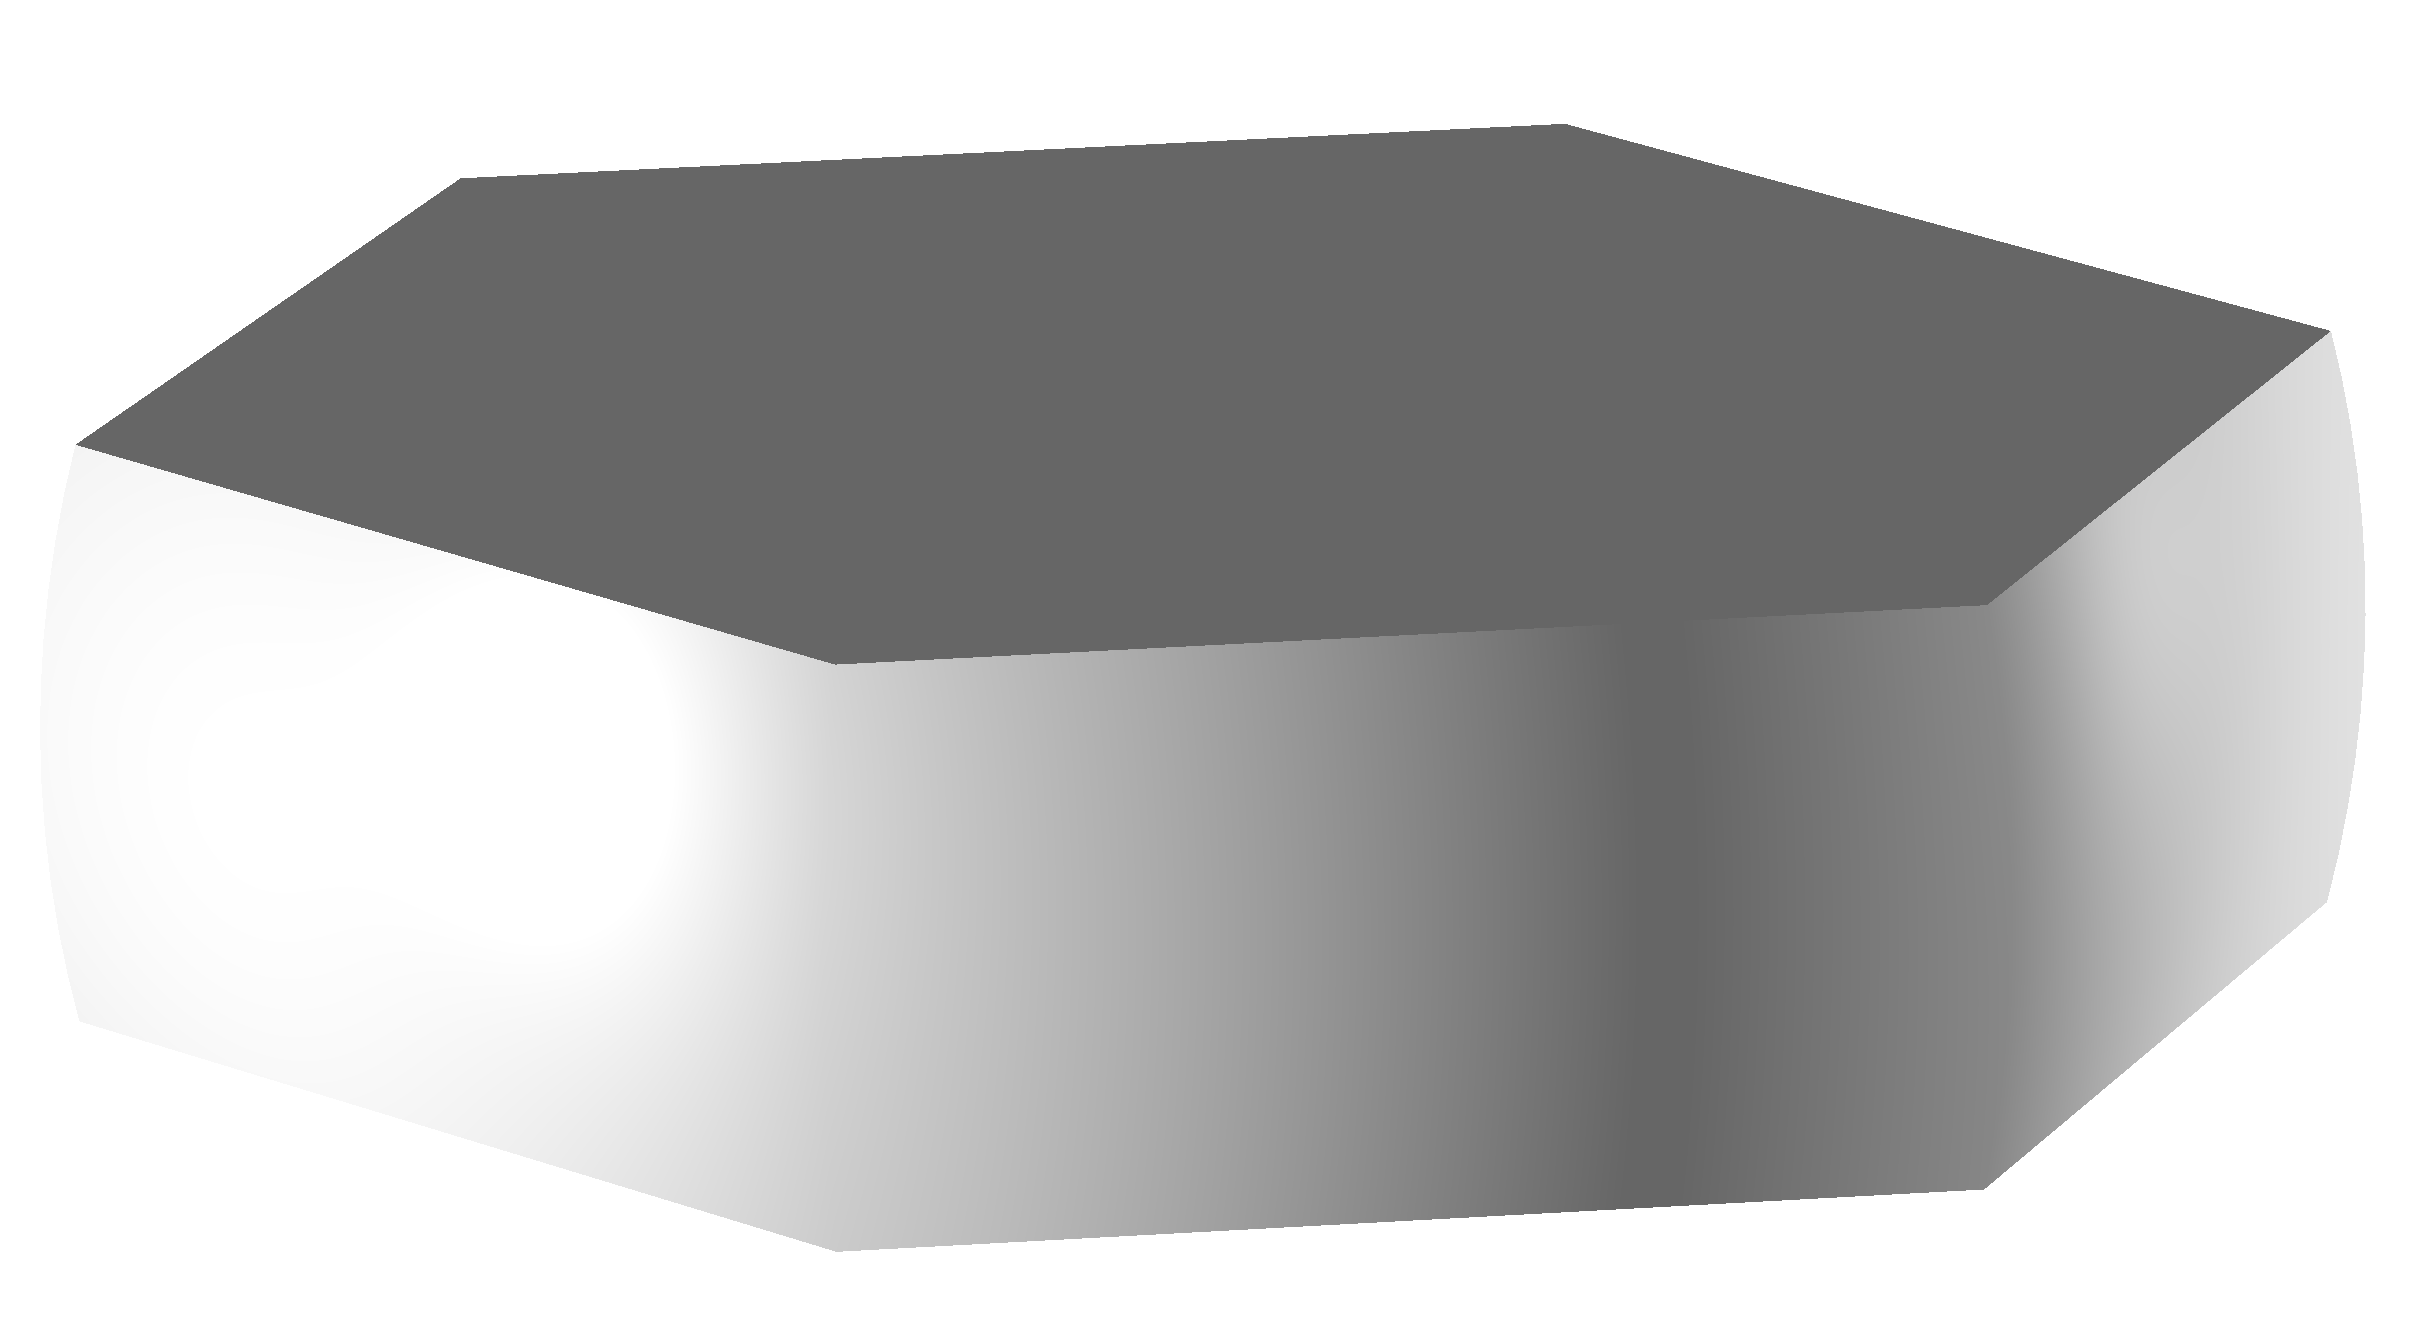
\includegraphics[width=\linewidth]{assets/images/shapes/bugold/scale_low}
    \caption{\makefirstuc{WebMGA 2.0}}
    \end{subfigure}
    \begin{subfigure}{0.2\textwidth}
    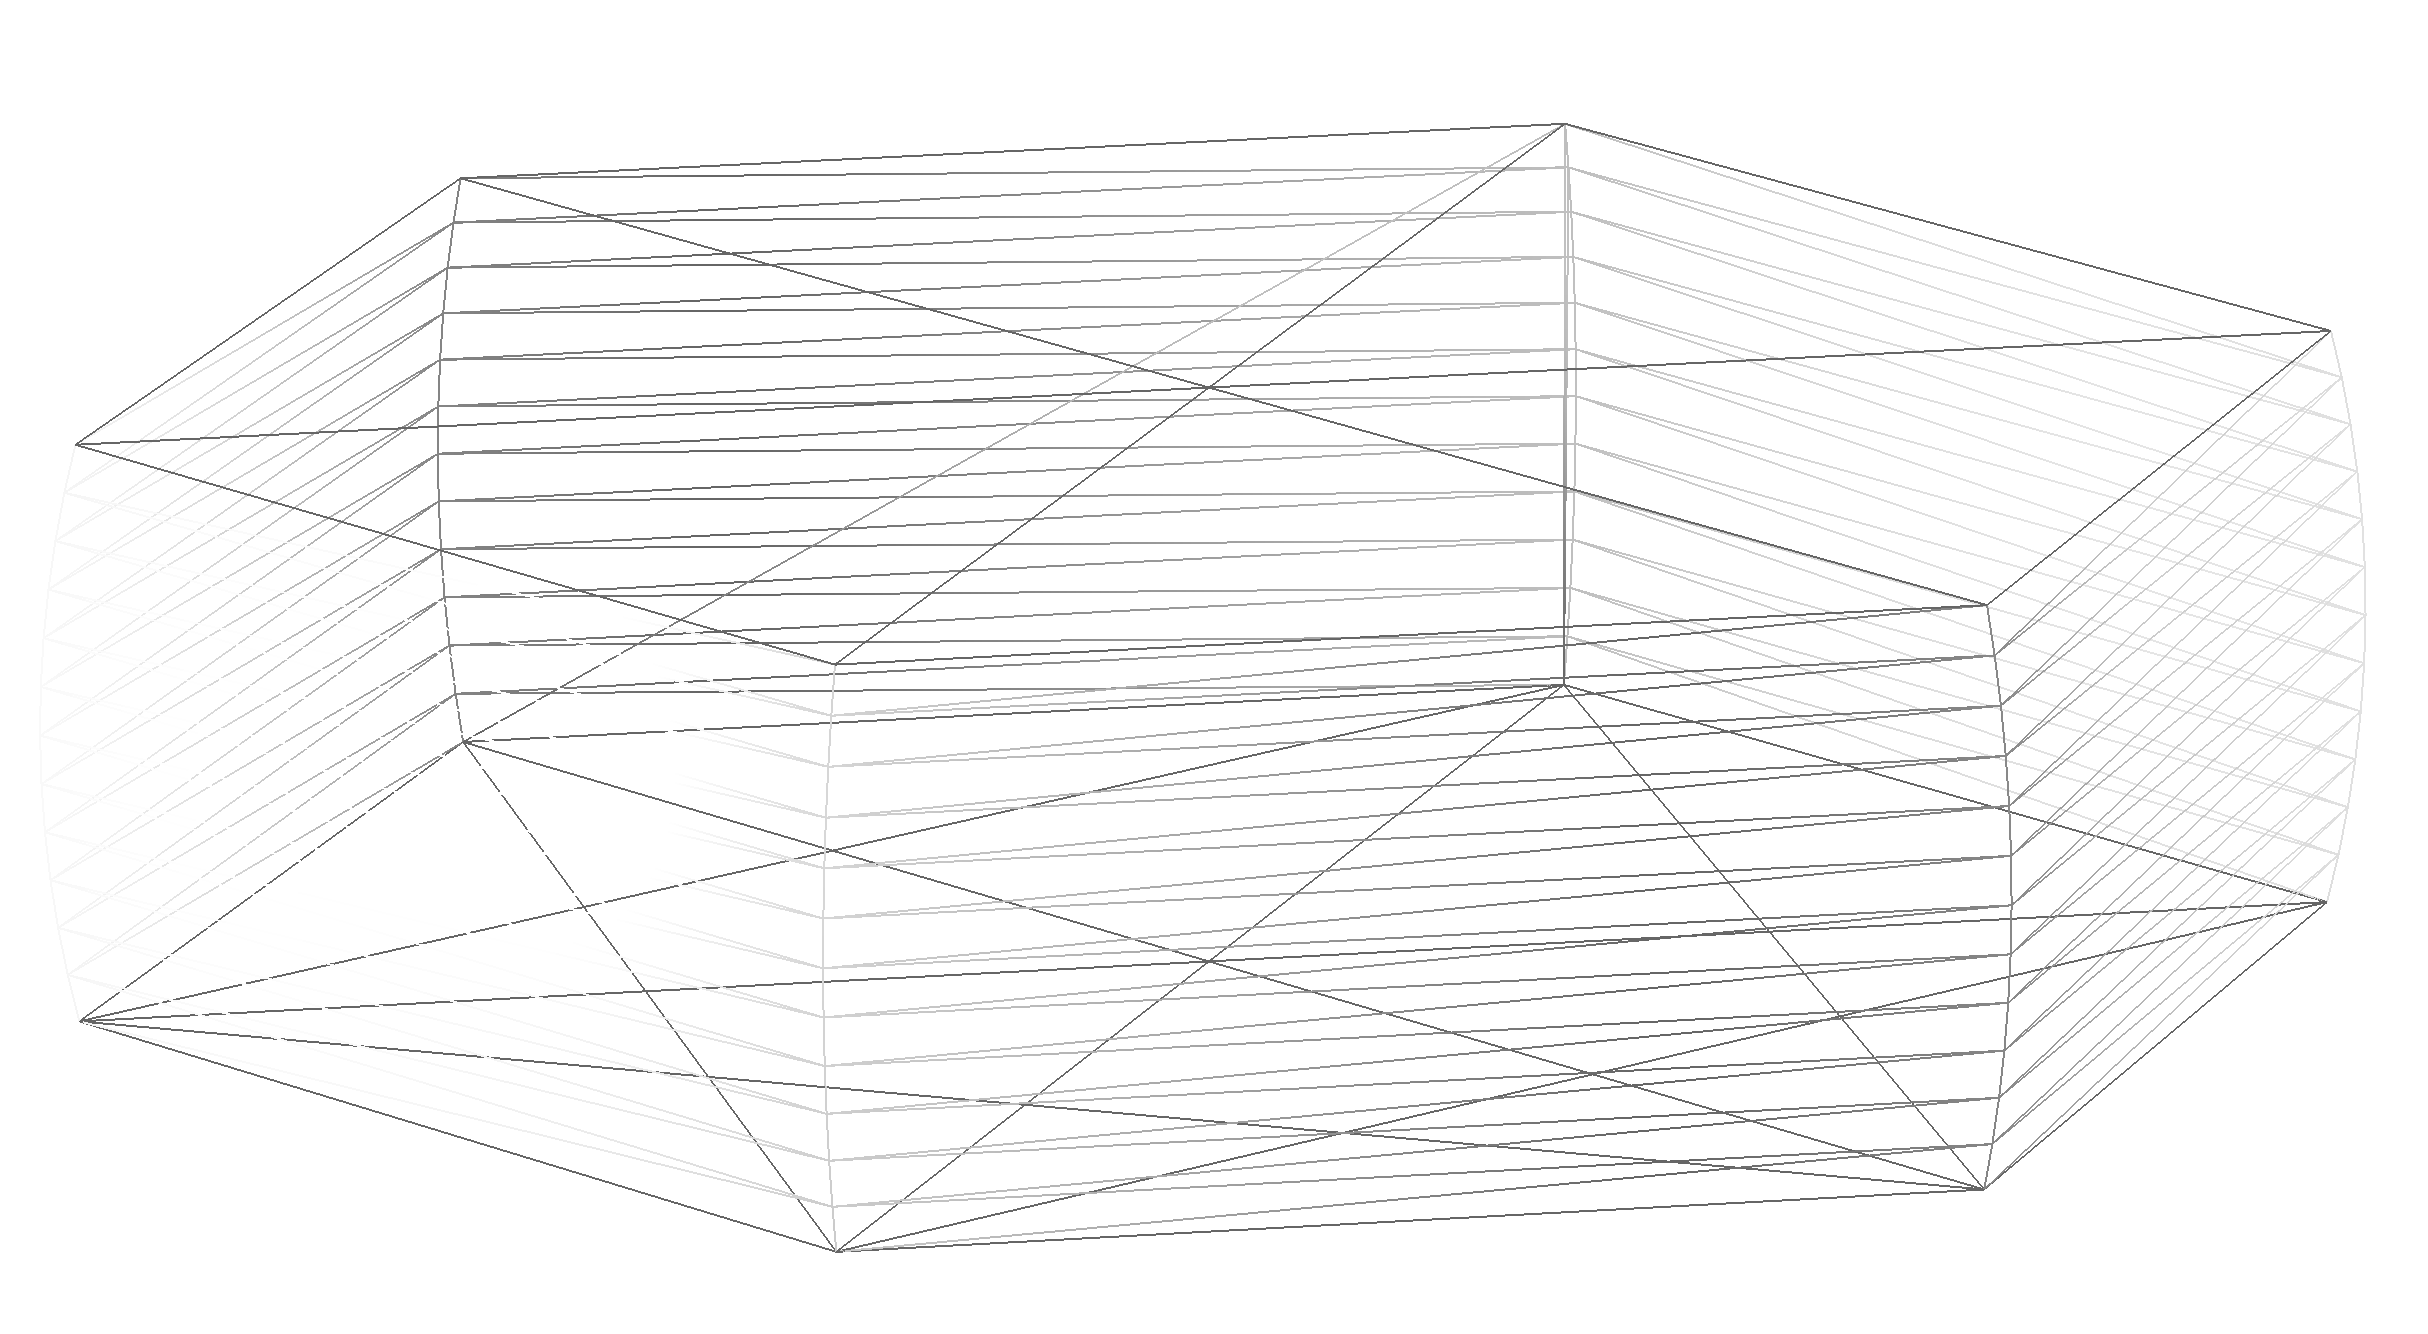
\includegraphics[width=\linewidth]{assets/images/shapes/bugold/scale_low_w}
    \caption{\makefirstuc{WebMGA 2.0}}
    \end{subfigure}
  \end{center}
  \caption{\makefirstuc{Notably higher mesh quality vertically for double cut sphere with WebMGA 2.0}}
  \label{fig:uneven_mesh_old}
\end{figure}
\begin{figure}
  \begin{center}
    \begin{subfigure}{0.4\textwidth}
    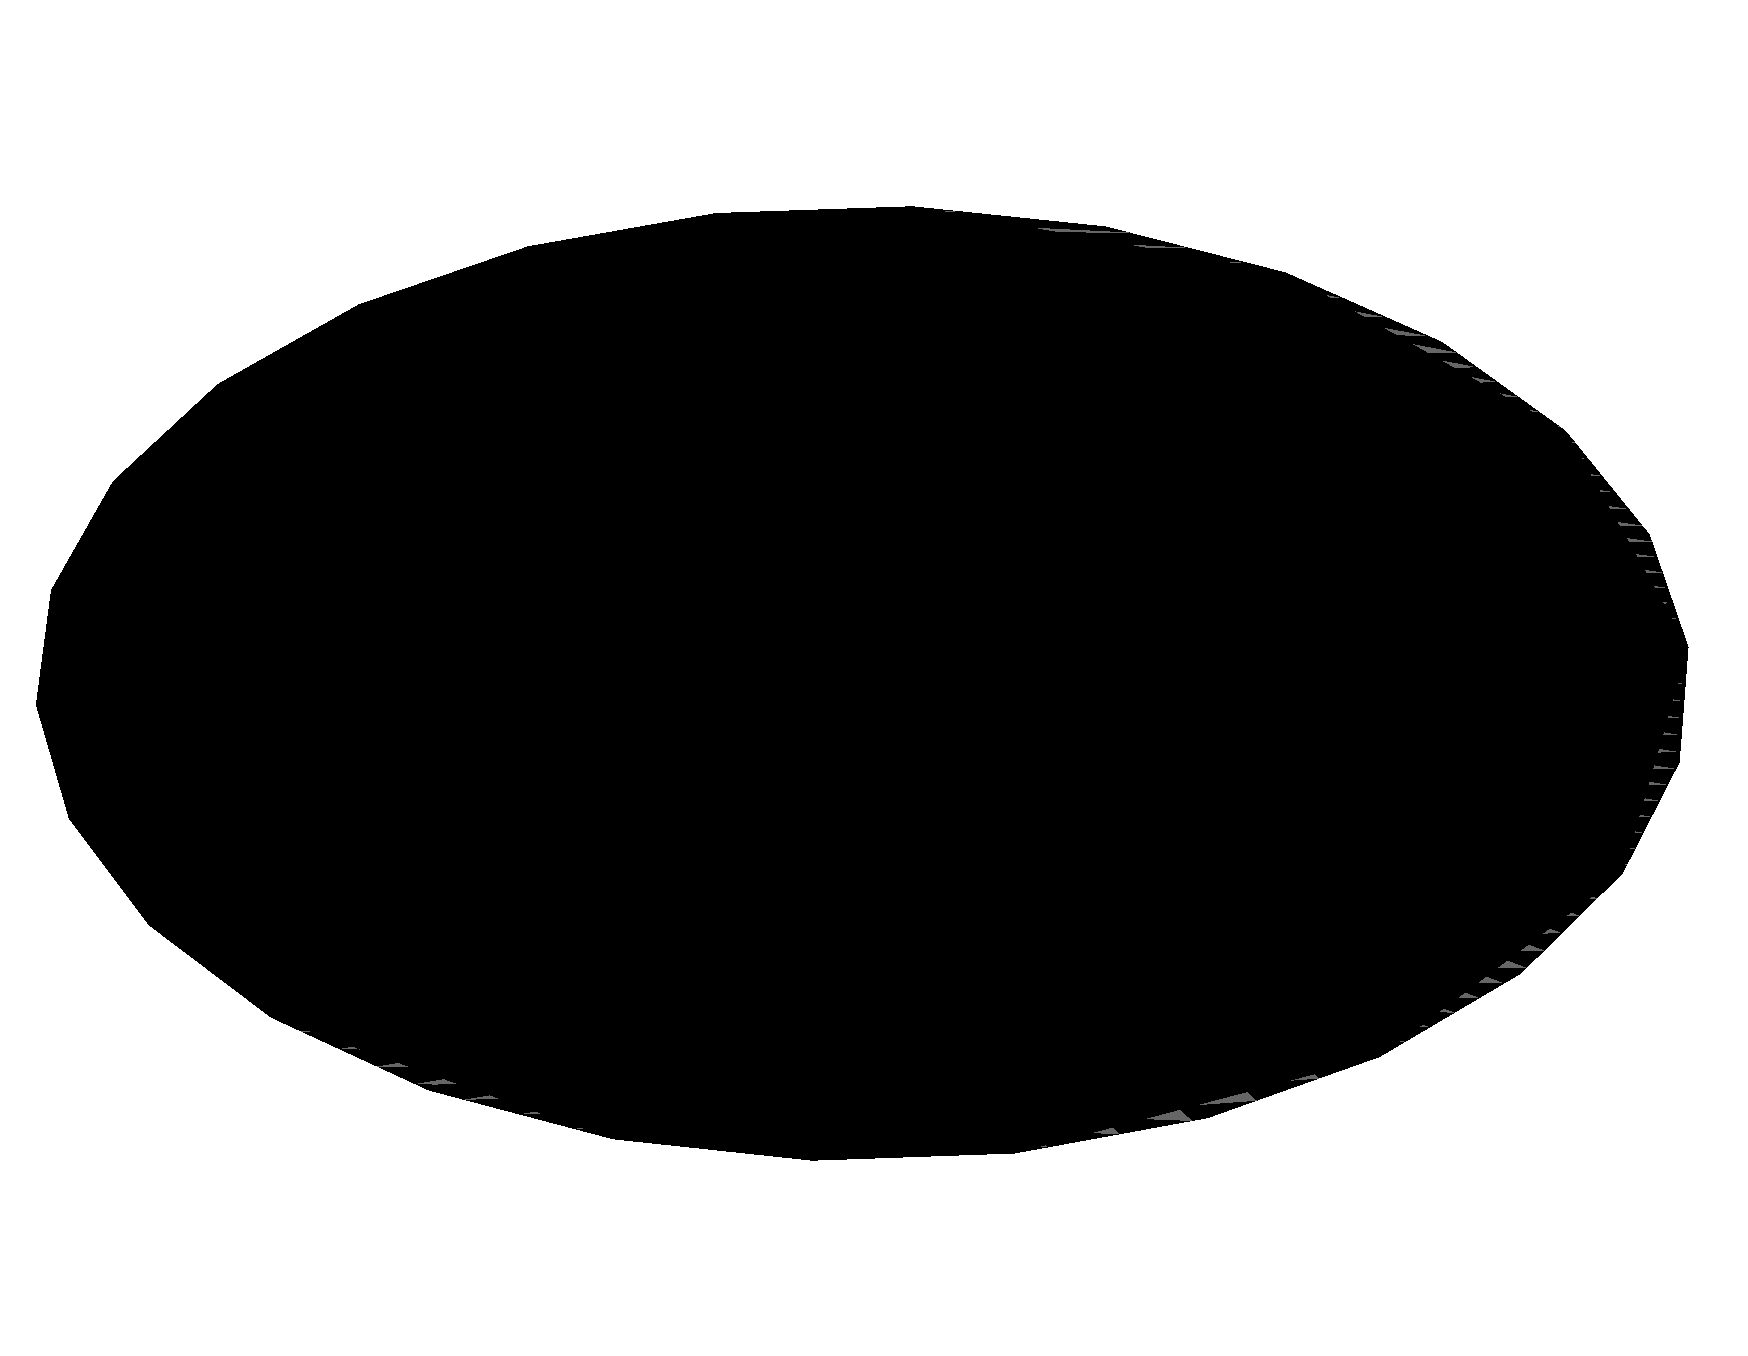
\includegraphics[width=\linewidth]{assets/images/shapes/bugold/no_height}
    \caption{\makefirstuc{WebMGA 2.0 Shape}}
    \end{subfigure}
    \begin{subfigure}{0.4\textwidth}
    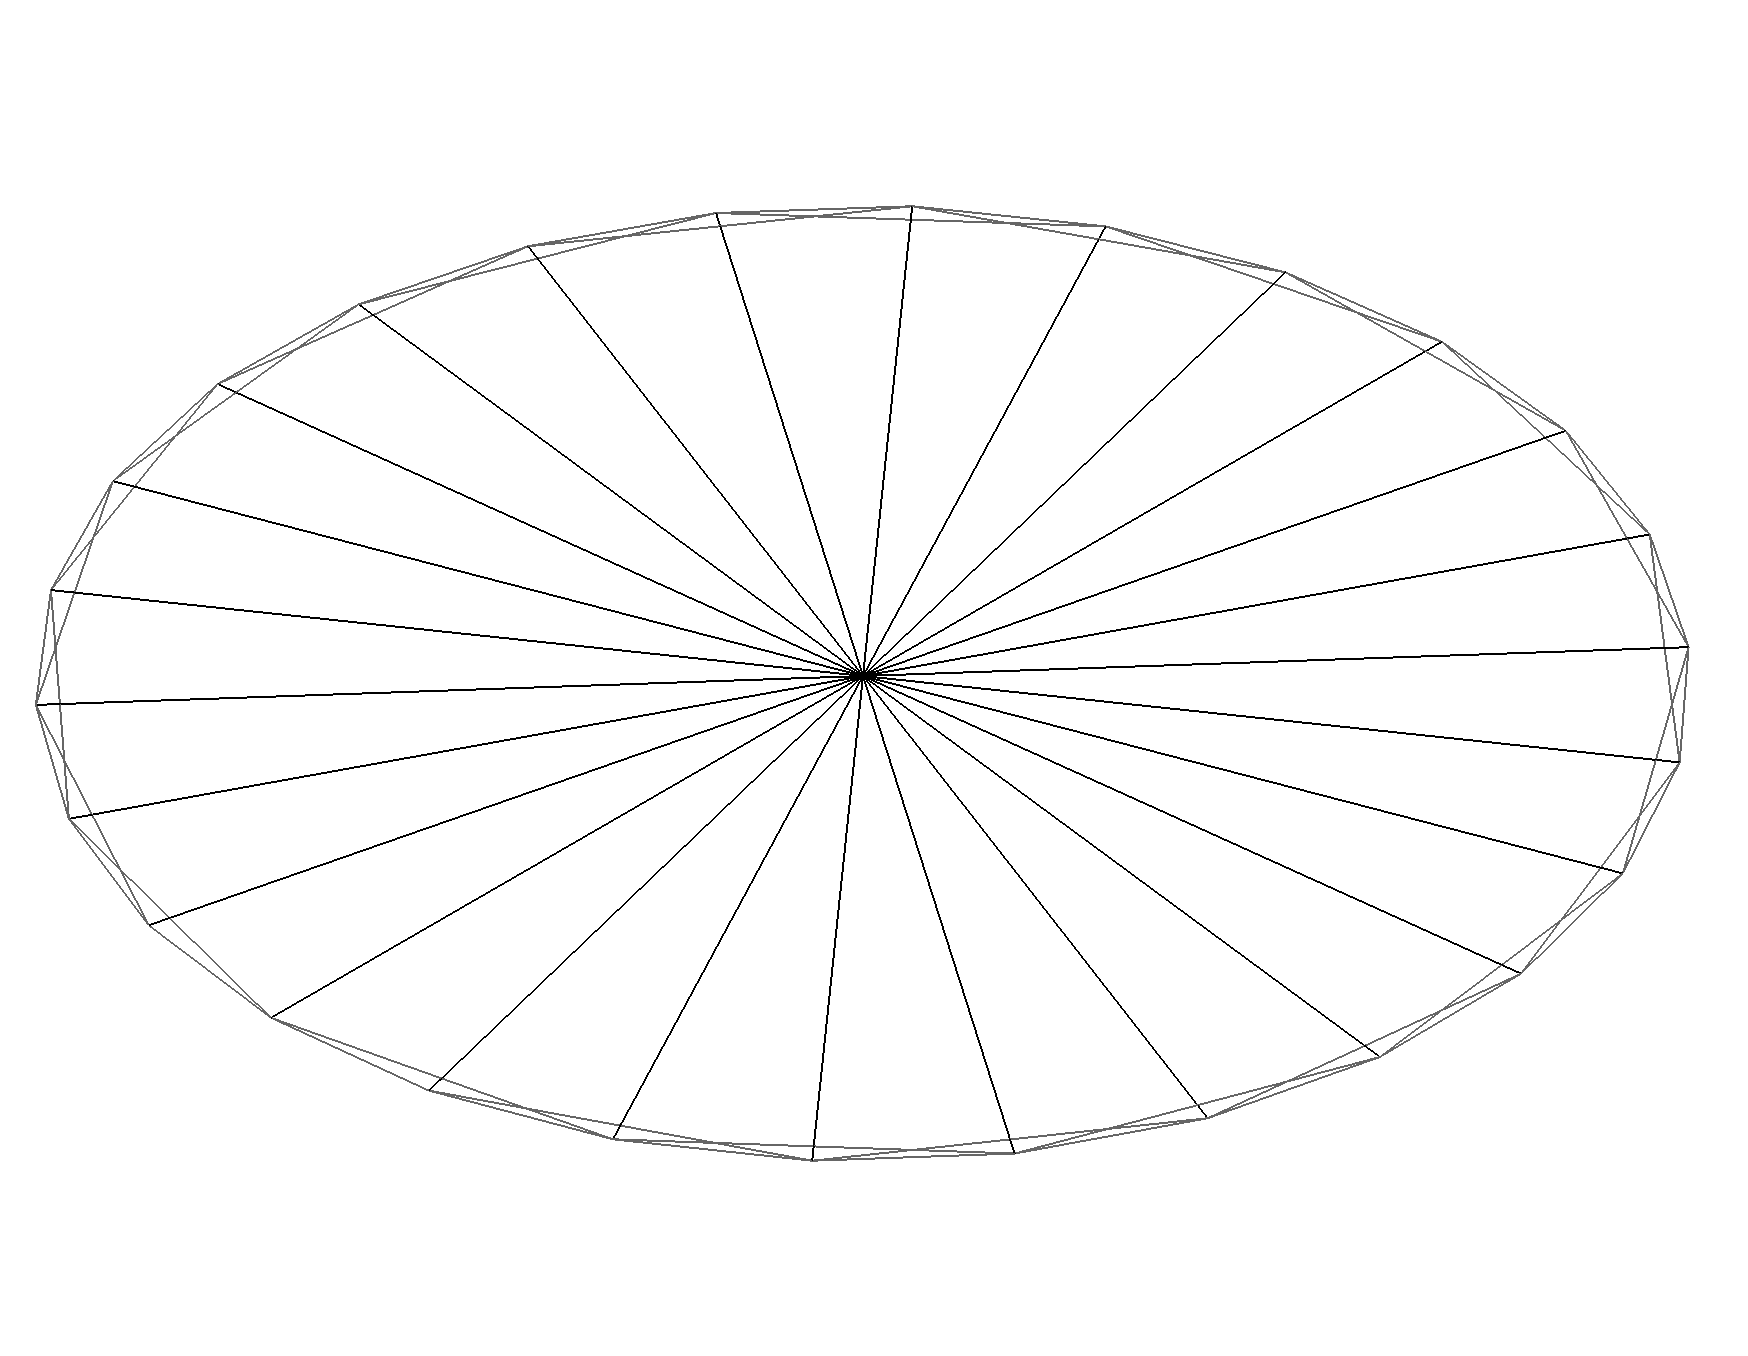
\includegraphics[width=\linewidth]{assets/images/shapes/bugold/no_height_w}
    \caption{\makefirstuc{WebMGA 2.0 Wireframe}}
    \end{subfigure}
    \begin{subfigure}{0.4\textwidth}
    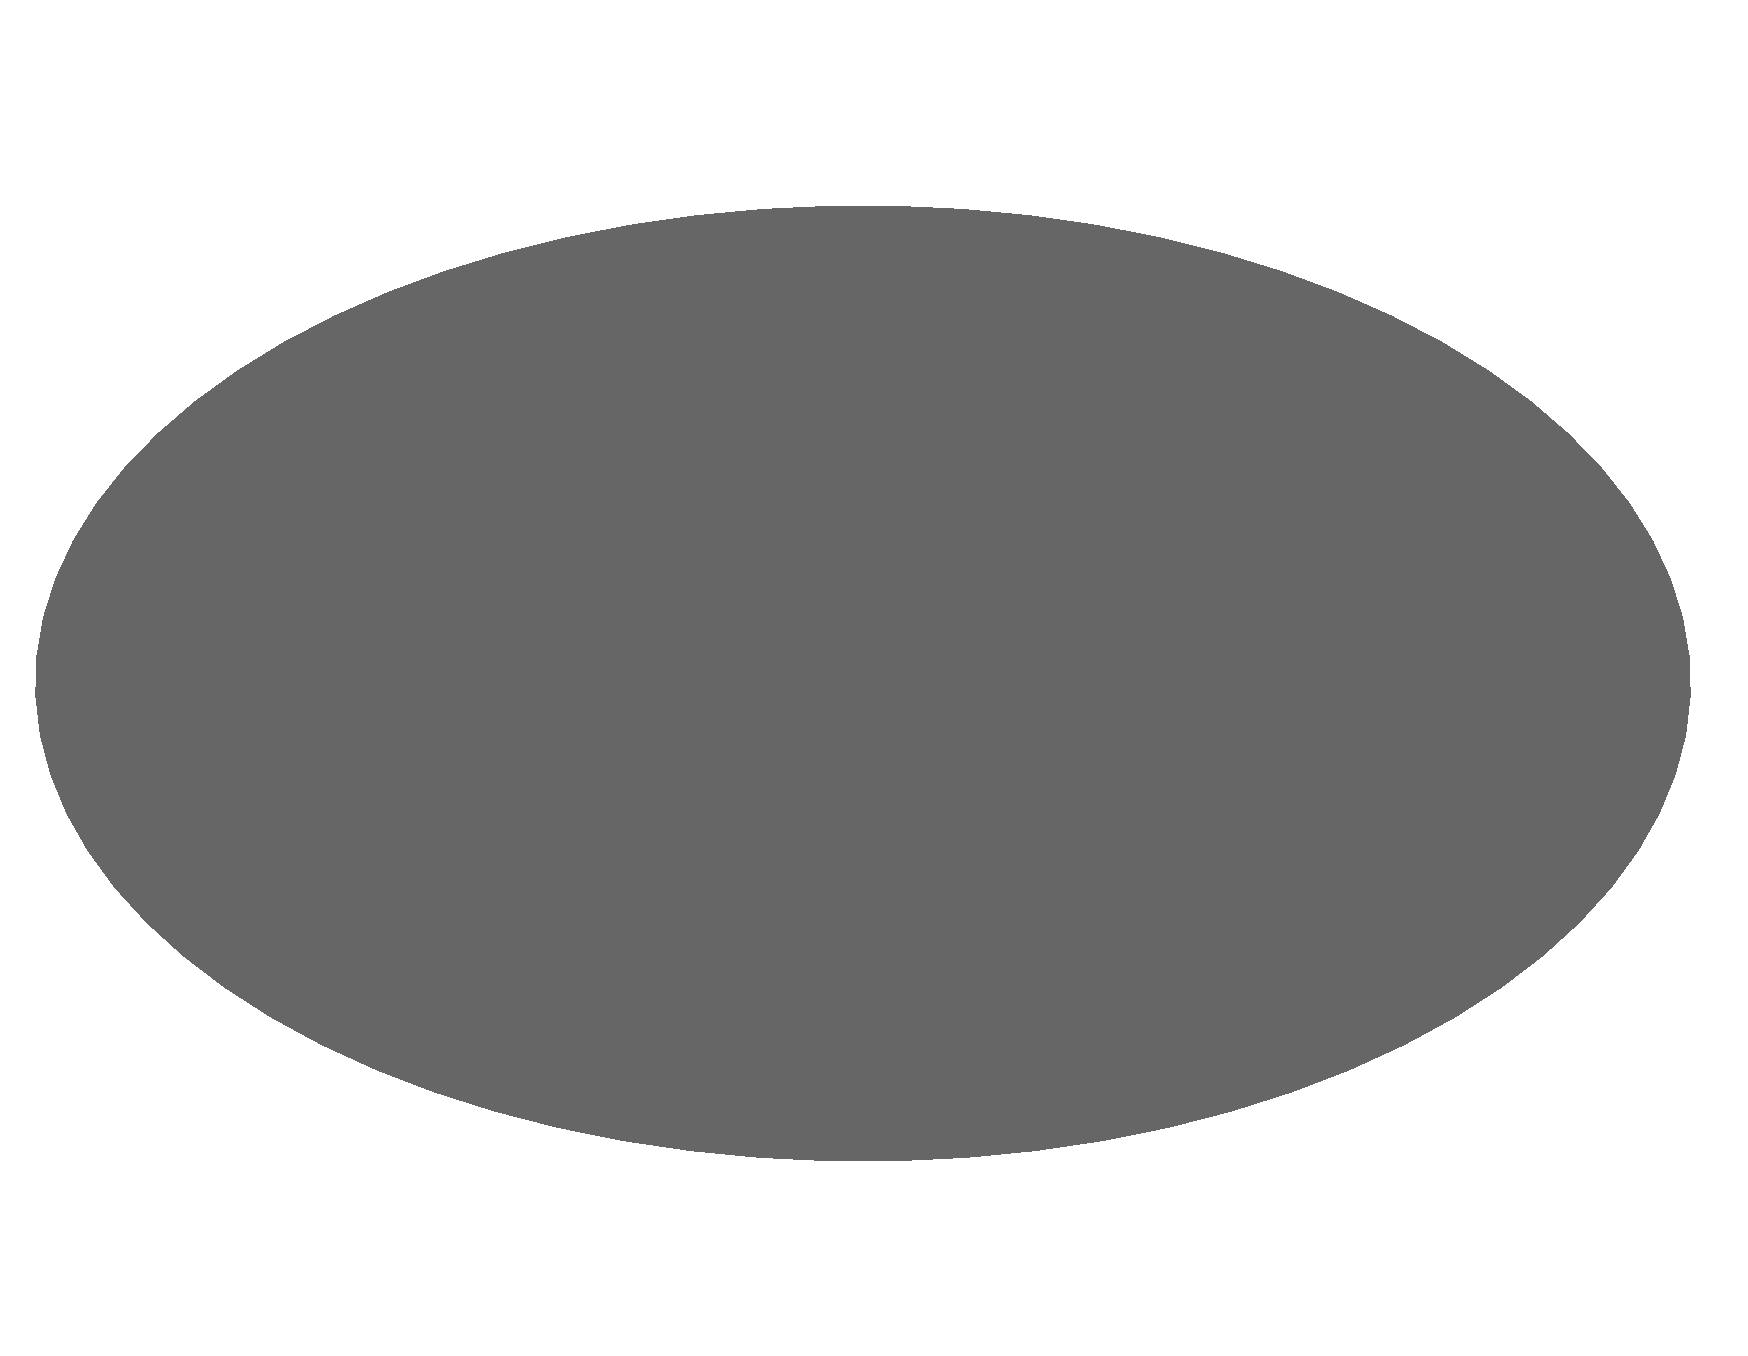
\includegraphics[width=\linewidth]{assets/images/shapes/bugnew/no_height}
    \caption{\makefirstuc{WebMGA 3.0 Shape}}
    \end{subfigure}
    \begin{subfigure}{0.4\textwidth}
    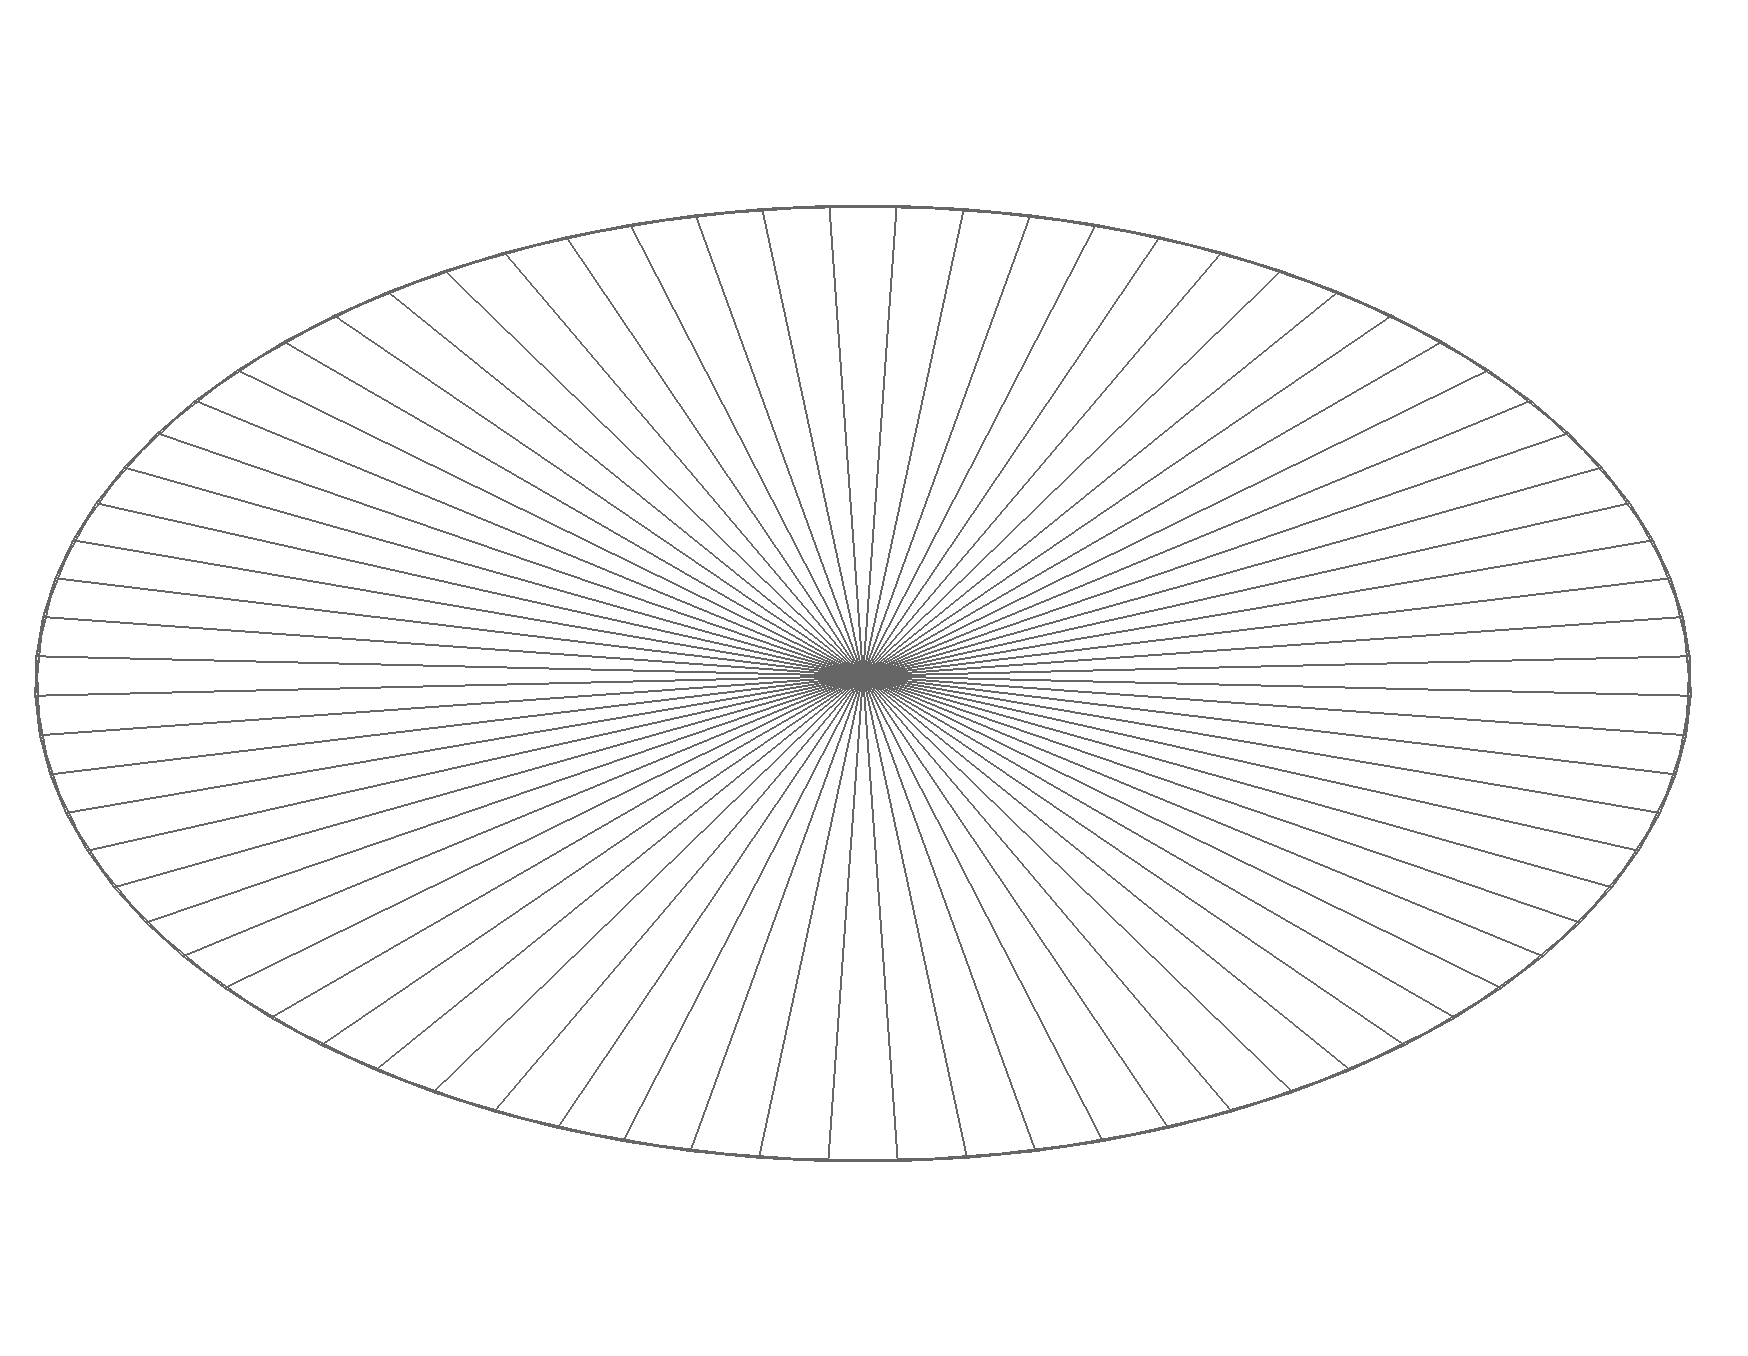
\includegraphics[width=\linewidth]{assets/images/shapes/bugnew/no_height_w}
    \caption{\makefirstuc{WebMGA 3.0 Wireframe}}
    \end{subfigure}
  \end{center}
  \caption{\makefirstuc{Buggy shape representation when double cut sphere has 0 height}}
  \label{fig:no_height_bug_old}
\end{figure}

\subsection{Improvement Goals}
\begin{itemize}
  \item Problem
    \begin{itemize}
      \item Fix
    \end{itemize}
\end{itemize}

\subsection{WebMGA 3.0 Implementation}
\subsubsection{Sphere}
\label{sphere_gen_sec}
Key to the new shape implementations is the implementation for the sphere (\cref{fig:sphere_shape}, parameter ``Radius''). The sphere mesh is generated by sampling points across the sphere's surface in such a way as to split it into a finite number of flat, triangular sub-faces as shown in \cref{fig:sphere_vertices}. This sampling is performed with the spherical coordinates system for some sphere radius $r$, azimuthal angles $\theta$, and polar angles $\phi$, converted to an equivalent Cartesian form. A point in spherical coordinate space is denoted $\mathbf{r}_{s}$, while a point in Cartesian space is denoted $\mathbf{r}_{C}$,

\begin{equation}
\mathbf{r}_\mathrm{s}=\begin{pmatrix}r\\\phi\\\theta\end{pmatrix}
\label{sphere_equation_spherical}
\end{equation}

\begin{equation}
\mathbf{r}_\mathrm{C}=\begin{pmatrix}r\sin\phi \cos\theta\\
r\sin\phi \sin\theta\\
r\cos\phi\end{pmatrix}
\label{sphere_equation_cartesian}
\end{equation}.

Any unique point on the origin centred $r$ sphere can be uniquely defined by some $(\theta,\phi)$ pair. Therefore, to evenly space points across the surface, a set of $\theta$s and $\phi$s is generated by taking $n$ (essentially a measure of mesh quality) evenly spaced values over the interval of a full circular rotation ($[0, 2\pi)$). Each unique pairing $(\phi,\gamma)$, along with $r$, is used to produce the full set of Cartesian vertices using \cref{sphere_equation_cartesian}. This method is sufficient to produce a sphere mesh as in \cref{fig:old_sphere} from WebMGA 2.0. The sampling is modified slightly for WebMGA 3.0 to produce a mesh as in \cref{fig:new_sphere} by offsetting each row such that points on one row lie half way between a pair of points on the row above since it produces a slightly more visually satisfying mesh. The code was rewritten from scratch since most other shapes result from slight modifications to the sphere generation process, and the initial WebMGA 2.0 implementation was over-complicated and proved difficult to extend.

TODO DISCUSS ORDERIGN AND FACES ETC.

Some optimisations are implemented to efficiently generate a full set of vertices while sampling only $\frac{1}{4}$ of the points around the sphere's surface. This uses the fact that the origin centred sphere is symmetrical in each of the $xy$, $xz$, and $yz$ planes. Points for the quarter sphere can be generated by applying \cref{sphere_equation_cartesian} with all pairings of $\frac{n}{2}$ evenly spaced $\theta \in [0, \pi)$, and $\frac{n}{2}$ evenly spaced $\phi \in [0, \frac{\pi}{2}]$. These points are arranged in a 3d array corresponding to rows (from $\phi$) and columns (from $\theta$).

An additional set of points for the diagonally opposite quarter is trivially generated with correct vertex ordering by copying the original quarter vertices and negating the $x$ and $y$ values for each vertex to mirror in the $xz$ and $yz$ planes. TODO FINISH 

TODO OPTIMISATION DIAGRAM

\begin{figure}
  \begin{center}
    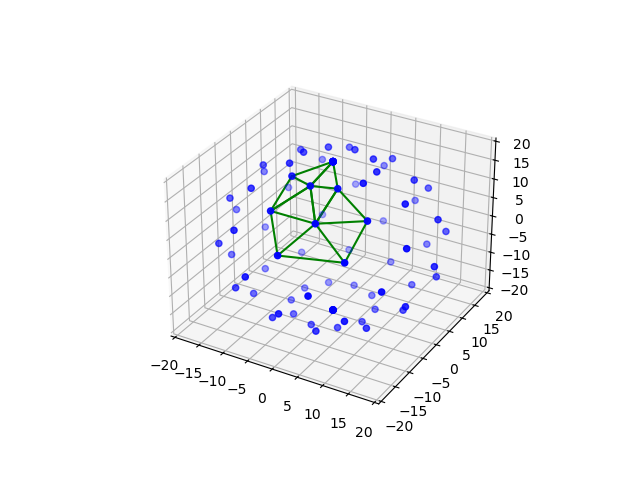
\includegraphics[width=0.5\linewidth]{assets/images/shapes/sphere_vertices}
    \caption{Example sphere vertex distribution ($9\times10$ vertical$\times$horizontal samples). Some mesh edges shown to demonstrate mesh construction from vertices.}
    \label{fig:sphere_vertices}
  \end{center}
\end{figure}

\shapefigure{sphere}{sphere}

\subsubsection{Ellipsoid}
The ellipsoid shape (\cref{fig:ellipsoid_shape}, parameters ``X'', ``Y'', ``Z'') can be represented as an origin centred sphere of radius 1 scaled in the $x$,$y$ and $z$ directions by some scalar value in each direction. This can be represented by a slightly modified form of the Cartesian sphere equation in \cref{sphere_equation_cartesian}, where $\mathbf{S}$ denotes some scaling vector,
\begin{equation}
\mathbf{r}_{e}=\begin{pmatrix}s_x r\sin\phi \cos\theta\\
s_y r\sin\phi \sin\theta\\
s_z r\cos\theta\end{pmatrix}
=\mathbf{S} \odot \mathbf{r}_\mathrm{C}
\label{ellipsoid_equation}
\end{equation}.
\shapefigure{ellipsoid}{ellipsoid}
From this formulation, it can be seen that an ellipsoid can be generated by slightly modifying the vertex sampling process for a sphere, whilst leaving the rest of the mesh building process unchanged. A sphere point can be sampled using \cref{sphere_equation_cartesian} with radius 1 and then multiplied by the scaling vector $\begin{pmatrix}s_x,s_y,s_z\end{pmatrix}^\mathsf{T}$ to give an equivalent result to \cref{ellipsoid_equation}.

In the program this is implemented by creating an ``Ellipsoid'' class as a child of the ``Sphere'' class and overriding the ``sample\_sphere()'' method. Since this implementation is so simple, the JavaScript code is provided below:

\begin{adjustbox}{width=\textwidth}
\begin{lstlisting}
//Ellipsoid mesh generator
export class Ellipsoid extends Sphere {
    //Scale factor in [x, y, z] directions
    scale: number[];

    constructor(x: number, y: number, z: number) {
        //Derive from origin centred sphere of radius 1
        super(1);
        this.scale = [x, y, z];
    }

    //Samples from ellipsoid instead of sphere
    sample_sphere(radius: number, theta: number, phi: number): number[] {
        //Multiply origin centred sphere coordinates by scale vector
        return math.dotMultiply(super.sample_sphere(radius, theta, phi), this.scale);
    }
}
\end{lstlisting}
\end{adjustbox}

\subsubsection{Spheroplatelet}
The spheroplatelet shape (\cref{fig:spheroplatelet_shape}, parameters ``RadSphere'' and ``RadCircle'') is generated by modifying a generates sphere mesh (see \cref{sphere_gen_sec}). Vertices are iterated over and pushed outwards by applying to the below formula, following on from \cref{sphere_equation_cartesian} with $c$ representing ``RadCircle'',$\mathbf{n}$ representing the sphere vertex normal in the $x,y$ plane, and $\mathbf{r}_{p}$ representing a vertex coordinate,
\begin{equation}
\mathbf{n}=\begin{pmatrix}
  r_x\\
  r_y
\end{pmatrix}
\end{equation}
\begin{equation}
\mathbf{r}_{p}=\mathbf{r}_C + \frac{c\mathbf{n}}{|\mathbf{n}|_2}.
\end{equation}

This will leave an empty circle of points at the top and bottom of the transformed geometry which can be filled by generating an additional vertices at the top and bottom respectively by averaging the coordinates for each vertex on the corresponding circle's edge, splitting it into triangles. This can be observed on \cref{fig:new_spheroplatelet_w}.
\shapefigure{spheroplatelet}{spheroplatelet}

\subsubsection{Cut Sphere}
\label{cut_sphere_section}
\begin{figure}
  \begin{center}
    \begin{subfigure}{0.3\textwidth}
      \includesvg[width=\textwidth]{assets/images/shape_diagrams/cut_sphere}
      \caption{Cut sphere.}
      \label{fig:cut_sphere_diagram}
    \end{subfigure}
    \begin{subfigure}{0.3\textwidth}
      \includesvg[width=\textwidth]{assets/images/shape_diagrams/doublecut}
      \caption{Double cut sphere.}
      \label{fig:double_cut_diagram}
    \end{subfigure}
    \begin{subfigure}{0.3\textwidth}
      \includesvg[width=\textwidth]{assets/images/shape_diagrams/cap}
      \caption{Cap.}
      \label{fig:cap_diagram}
    \end{subfigure}
  \end{center}
  \caption{Cap and cut sphere shape diagrams. Lens outlines are shown by a red line, black lines demonstrate construction.}
  \label{fig:cap_cut_descriptions}
\end{figure}
The cut sphere shape (\cref{fig:cutsphere_shape}, parameters ``Radius'', ``zCut'') is implemented simply by sampling the sphere as before but over a reduced range of $\phi$ values. Since the sphere will not be completed, an empty circular face is left which can be filled by generating an additional vertex by averaging the coordinates for each vertex on the circle's edge, splitting it into triangles. This can be observed on \cref{fig:new_cutsphere_w}.

A cut sphere is parameterised in WebMGA using a parent sphere radius and a zCut distance. These are shown in \cref{fig:cut_sphere_diagram}, with characters $r$ and $x$ respectively. The new range of $\phi$s can be seen in the diagram as the range $[\alpha,\pi)$, which can be reinterpreted in terms of $r$ and $x$ as follows,
\begin{equation}
\alpha=\arcsin\frac{c}{r}
\end{equation}
\begin{equation}
c=\sqrt{r^2-x^2}
\end{equation}
\begin{equation}
[\alpha,\pi)=[\arcsin\frac{c}{r},\pi)
\end{equation}

\newshapefigure{cutsphere}{cut sphere}

\subsubsection{Double Cut Sphere}
The double cut sphere shape (\cref{fig:doublecutsphere_shape}, parameters ``Radius'', ``zCut'') is implemented simply by sampling the sphere as before but over a reduced range of $\phi$ values. Since the sphere will not be completed, two empty circular faces are left which can be filled by generating two additional vertices by averaging the coordinates for each vertex on the corresponding circle's edge, splitting it into triangles. This can be observed on \cref{fig:new_doublecutsphere_w}.

A double cut sphere is parameterised in WebMGA using a parent sphere radius and a zCut distance. These are shown in \cref{fig:double_cut_diagram}, with characters $r$ and $x$ respectively. The new range of $\phi$s can be seen in the diagram as the range $[\alpha,\pi-\alpha)$, which can be reinterpreted in terms of $r$ and $x$ as follows,
\begin{equation}
\alpha=\arcsin\frac{c}{r}
\end{equation}
\begin{equation}
c=\sqrt{r^2-x^2}
\end{equation}
\begin{equation}
[\alpha,\pi-\alpha)=[\arcsin\frac{c}{r},\pi - \arcsin\frac{c}{r})
\end{equation}
\shapefigure{doublecutsphere}{double cut sphere}

\subsubsection{Cap}
\label{cap_section}
\newshapefigure{cap}{cap}
The cap shape (\cref{fig:cap_shape}, parameters ``Radius'', ``zCut'') is implemented simply by sampling the sphere as before but over a reduced range of $\phi$ values. Since the sphere will not be completed, an empty circular face is left which can be filled by generating an additional vertex by averaging the coordinates for each vertex on the circle's edge, splitting it into triangles. This can be observed on \cref{fig:new_cap_w}.

A cap is parameterised in WebMGA using a parent sphere radius and a zCut distance. These are shown in \cref{fig:cap_diagram}, with characters $r$ and $x$ respectively. The new range of $\phi$s can be seen in the diagram as the range $[0,\alpha)$, which can be reinterpreted in terms of $r$ and $x$ as follows,
\begin{equation}
\alpha=\arcsin\frac{c}{r}
\end{equation}
\begin{equation}
c=\sqrt{r^2-x^2}
\end{equation}
\begin{equation}
[0, \alpha)=[0, \arcsin\frac{c}{r})
\end{equation}

\subsubsection{Lens}
\begin{figure}
  \begin{center}
    \begin{subfigure}{0.3\textwidth}
      \includesvg[width=\textwidth]{assets/images/shape_diagrams/lens}
      \caption{Lens.}
      \label{fig:lens_diagram}
    \end{subfigure}
    \begin{subfigure}{0.3\textwidth}
      \includesvg[width=\textwidth]{assets/images/shape_diagrams/cinacchi}
      \caption{Cinacchi lens.}
      \label{fig:cinacchi_lens_diagram}
    \end{subfigure}
    \begin{subfigure}{0.3\textwidth}
      \includesvg[width=\textwidth]{assets/images/shape_diagrams/biconvex}
      \caption{Biconvex lens.}
      \label{fig:biconvex_lens_diagram}
    \end{subfigure}
  \end{center}
  \caption{Lens shape diagrams. Lens outlines are shown by a red line, black lines demonstrate construction.}
  \label{fig:lens_descriptions}
\end{figure}

The lens shape (\cref{fig:lens_shape}, parameters ``Radius'', ``Thickness'', ``Angle'') is created by assembling either two caps (\cref{cap_section}) or a cap and a a cut sphere (\cref{cut_sphere_section}) to recreate the format shown in \cref{fig:lens_diagram}. For the upper part of the lens, a cap is generated with angle parameter $\alpha$. For the lower part of the lens, if the required $\theta$ is greater than $\frac{\pi}{2}$ then a TODO FINISH
\paragraph{Base Lens}
\label{base_lens_para}
\paragraph{Thick Lens}
\newshapefigure{lens}{lens}

\subsubsection{Cinacchi Lens}
During development, some sample configurations requiring the lens molecule shape were provided by Giorgio Cinacchi. This is named the ``Cinacchi Lens'' in WebMGA (parameters ``Radius''). For these configurations, Cinacchi uses a specific lens configuration as shown in \cref{fig:cinacchi_lens_diagram} which is parameterised using only a single $r$ value,
\begin{equation}
\cos\theta=1-\frac{1}{2\pi r^2}
\label{cinacchi_equations_1}
\end{equation}
\begin{equation}
\theta=\arccos\left(1-\frac{1}{2\pi r^2}\right).
\label{cinacchi_equations_2}
\end{equation}
This produces an infinitely thin lens with some aperture angle dependent on the radius. The Cinnachi lens is implemented simply as a parameterisation of the base lens in \cref{base_lens_para} where the two radii are both $r$, and the angle is derived from \cref{cinacchi_equations_2}.

A screenshot produced using QMGA was provided by Cinacchi to assist in visually verifying the shape produced. This is shown in \cref{fig:cinacchi_lens_provided}. A recreation was produced in QMGA as shown in \cref{fig:cinacchi_lens_qmga}, then WebMGA as shown in \cref{fig:cinacchi_lens_webmga}. This appears to verify a correct implementation.

\begin{figure}
  \begin{center}
    \begin{subfigure}{0.3\textwidth}
      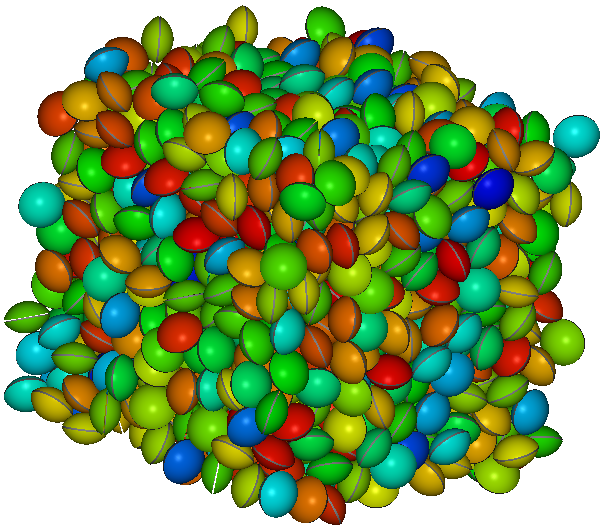
\includegraphics[width=\textwidth]{assets/images/cinacchi}
      \caption{Image by Giorgio Cinacchi.}
      \label{fig:cinacchi_lens_provided}
    \end{subfigure}
    \begin{subfigure}{0.3\textwidth}
      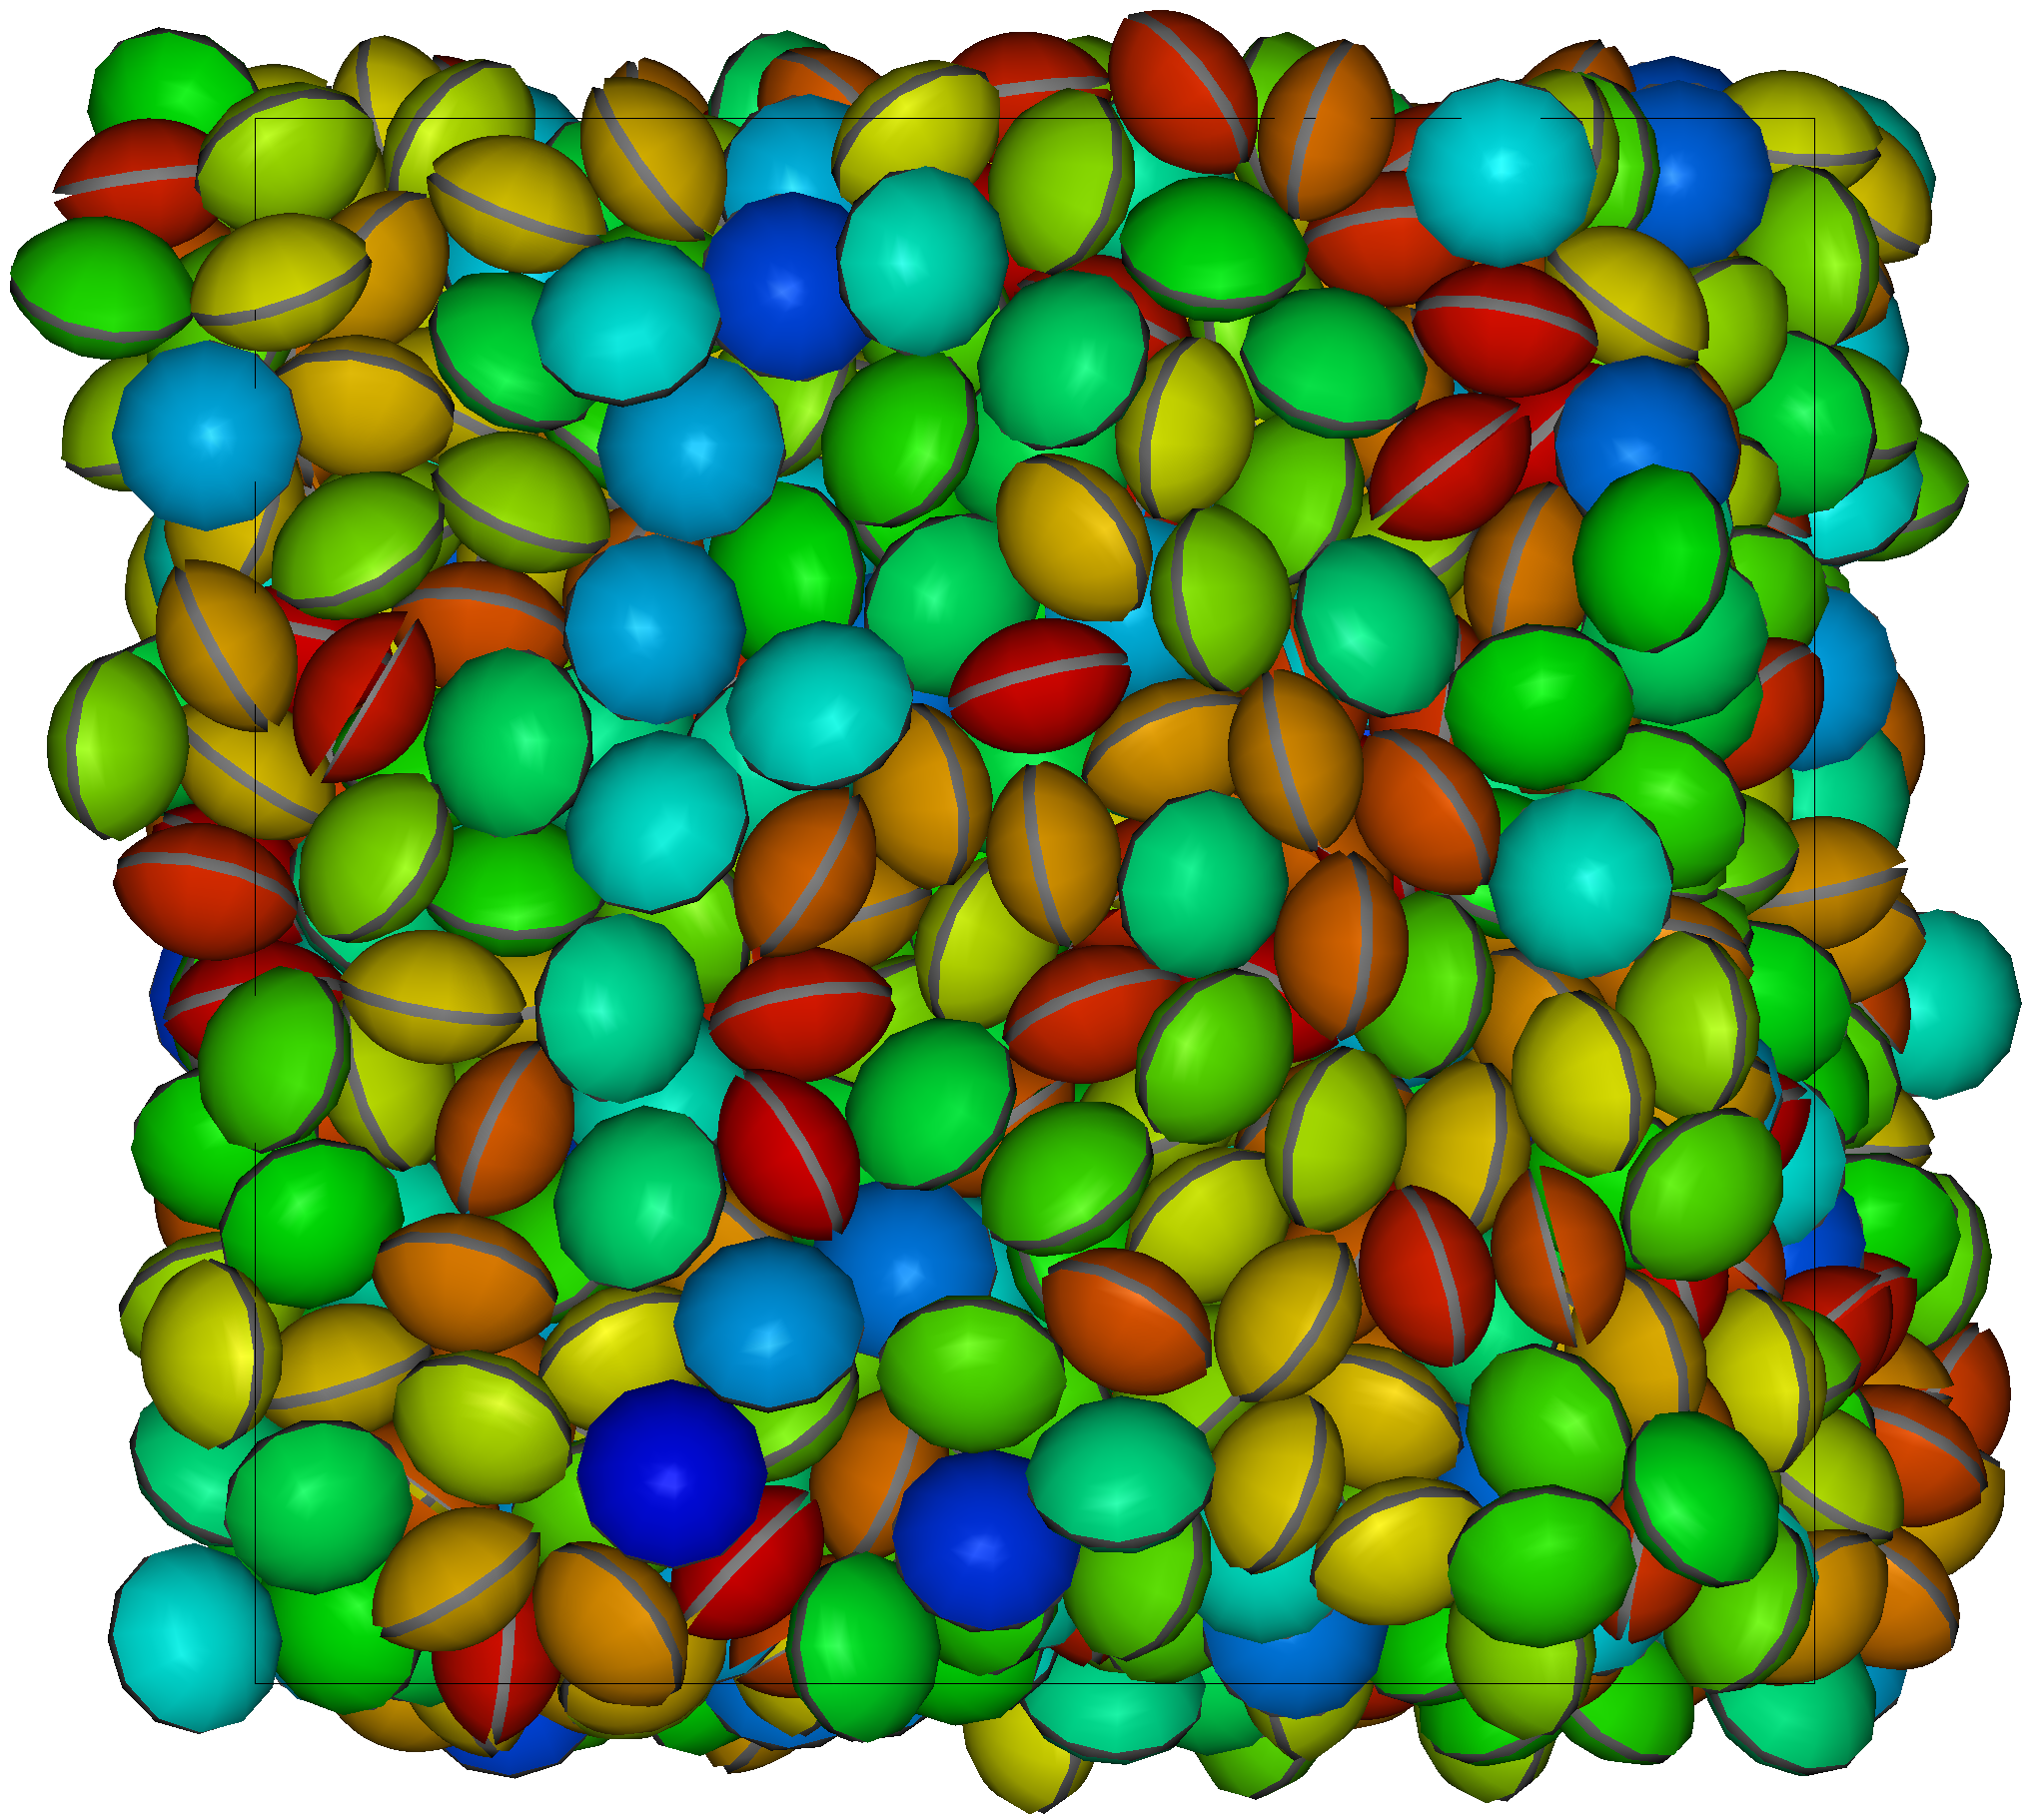
\includegraphics[width=\textwidth]{assets/images/qmga}
      \caption{Recreation with QMGA.}
      \label{fig:cinacchi_lens_qmga}
    \end{subfigure}
    \begin{subfigure}{0.3\textwidth}
      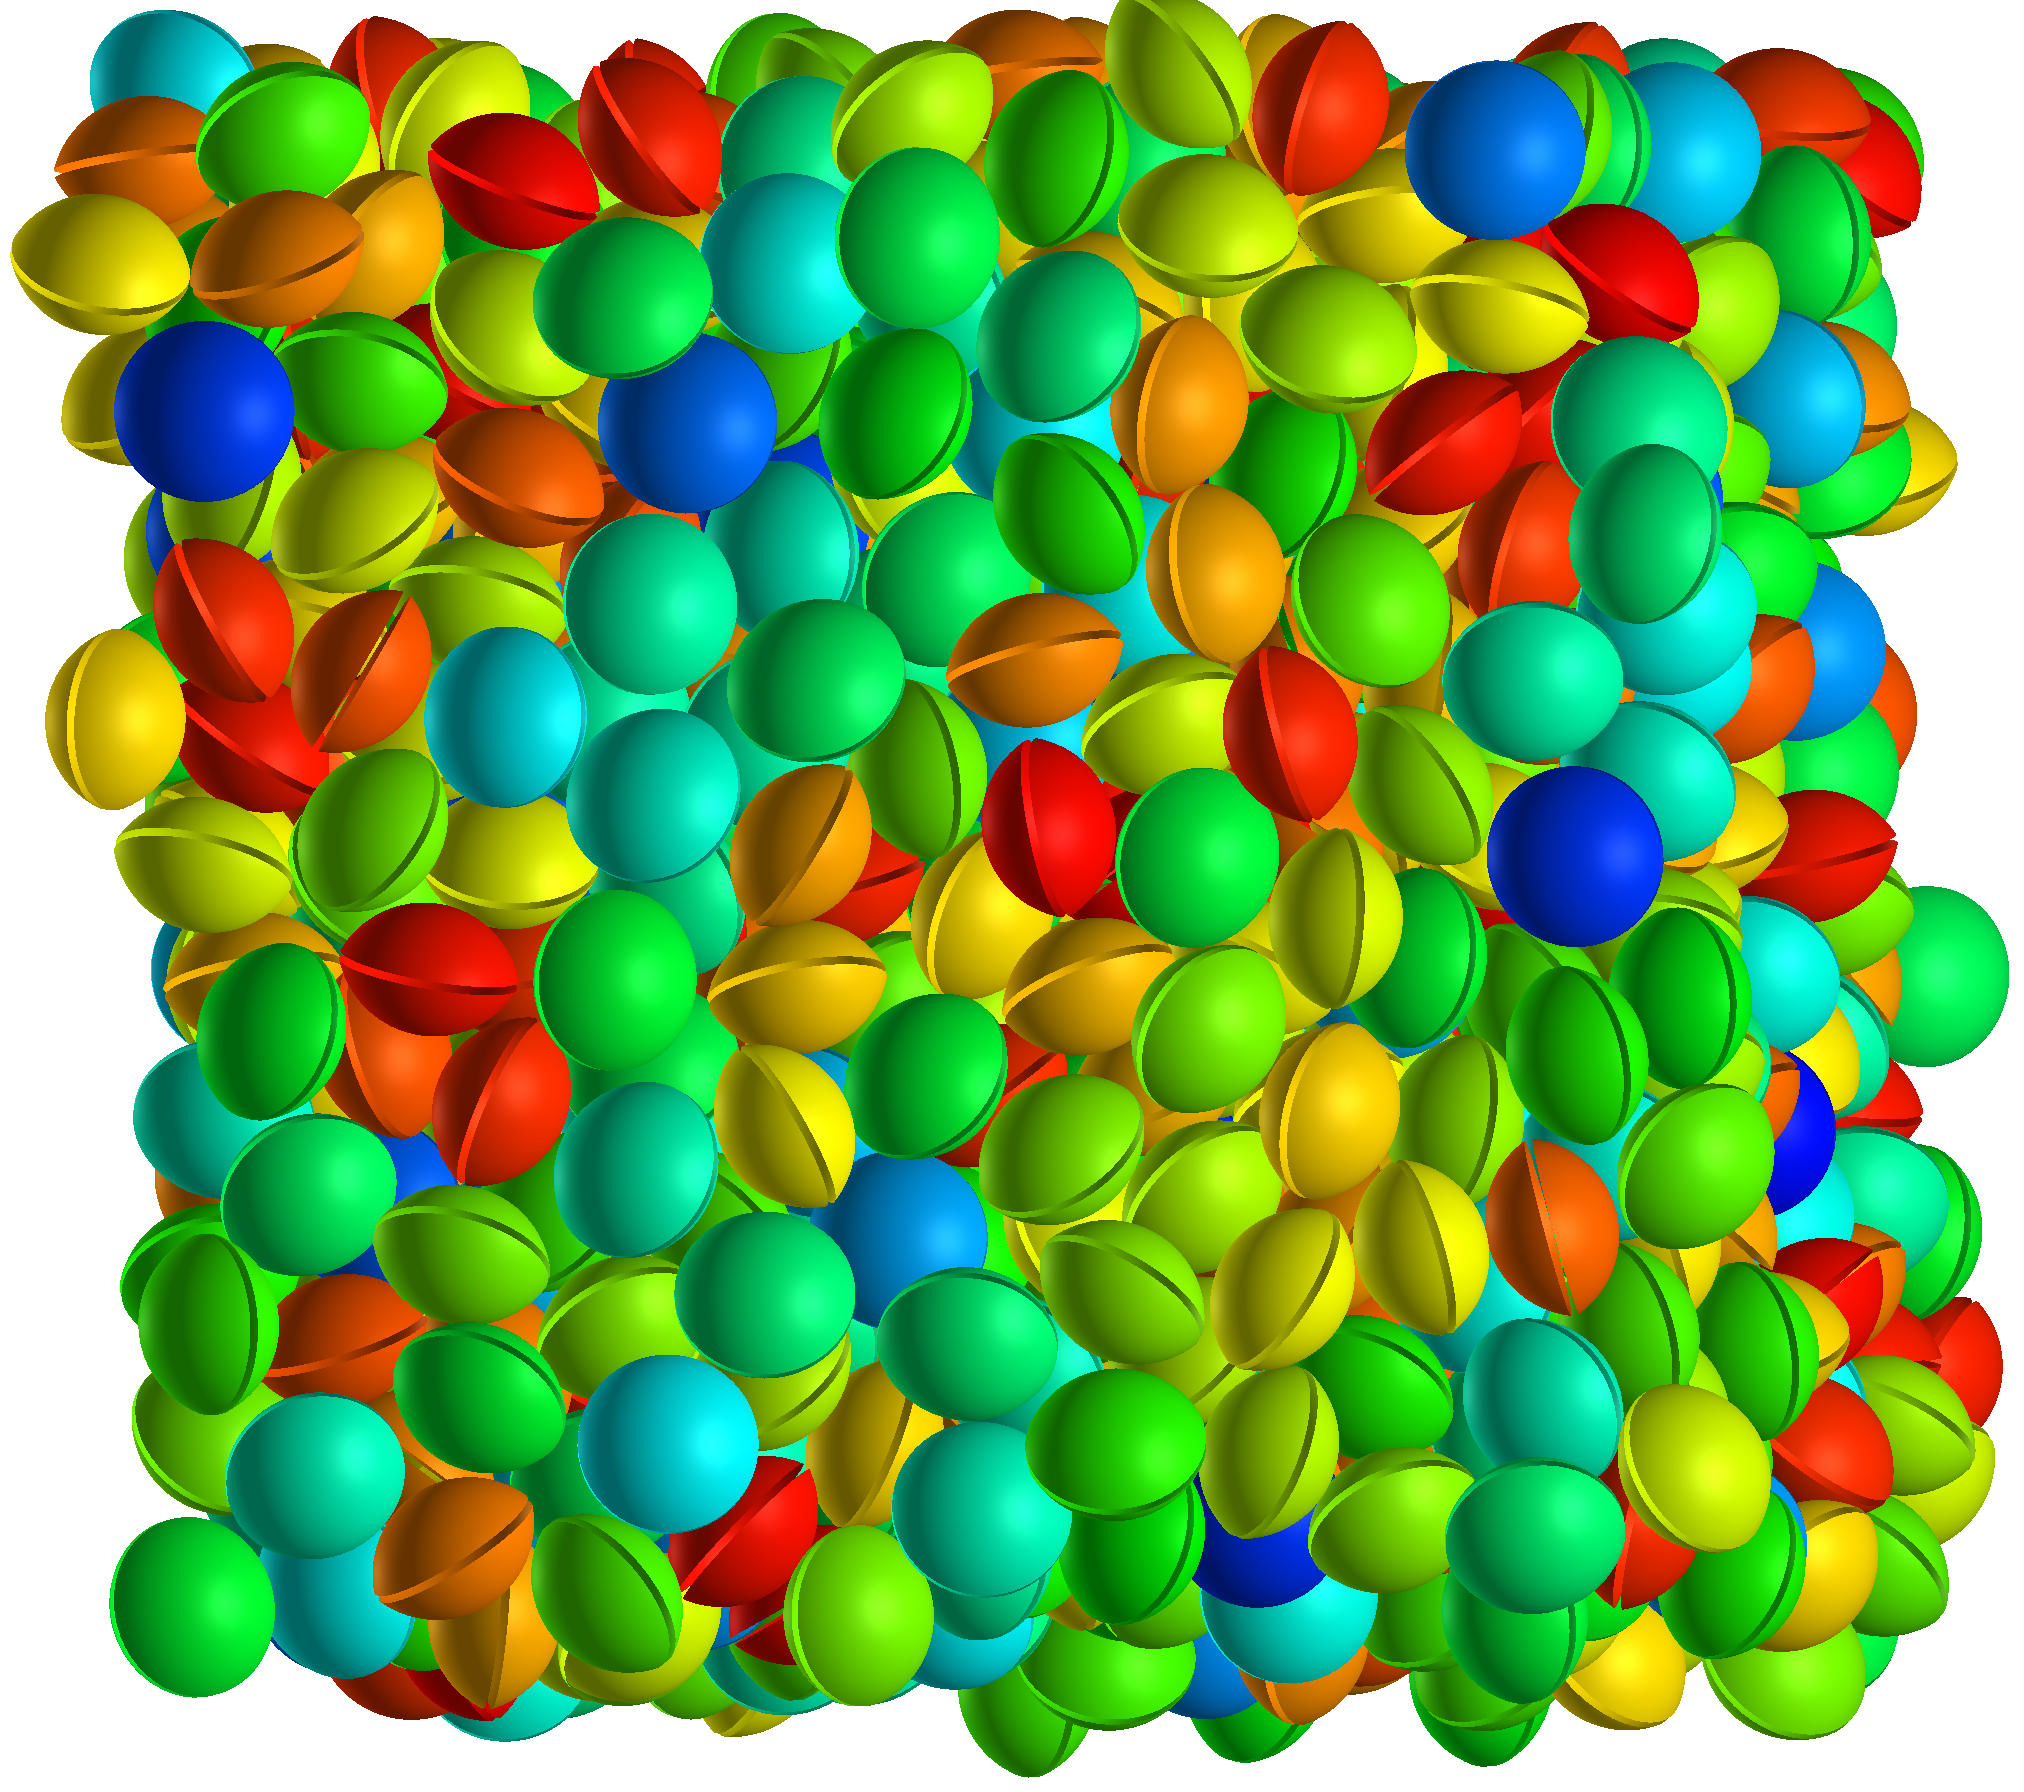
\includegraphics[width=\textwidth]{assets/images/webmga}
      \caption{Recreation with WebMGA.}
      \label{fig:cinacchi_lens_webmga}
    \end{subfigure}
  \end{center}
  \caption{Lens setup required by Giorgio Cinacchi.}
  \label{fig:cinacchi_lens}
\end{figure}

\subsubsection{Biconvex Lens}
\label{biconvex_section}
%\newshapefigure{}{}

\subsubsection{Spherocylinder}
\label{spherocylinder_section}
The spherocylinder shape (\cref{fig:spherocylinder_shape}, parameters ``Radius'', ``Length'') can be represented as an origin centred sphere of radius $r$ scaled in the $z$ directions by (half of) some length value in each $z$ direction (positive/negative). This can be represented by a slightly modified form of the Cartesian sphere equation in \cref{sphere_equation_cartesian},

\begin{equation}
\mathbf{r}_{c}=\begin{pmatrix}r\sin\phi \cos\theta\\
r\sin\phi \sin\theta\\
r\cos\theta + n\end{pmatrix}
=\mathbf{r}_{C}+\begin{pmatrix}0\\
0\\
n\end{pmatrix}
\label{spherocylinder_equation}
\end{equation}
\begin{equation}
n=\begin{cases}
  \frac{\text{length}}{2}&\text{if } r\cos\theta>0\\
  -\frac{\text{length}}{2}&\text{if } r\cos\theta<0\\
  0&\text{otherwise.}
\end{cases}
\label{spherocylinder_n_equation}
\end{equation}.
\paragraph{Initial Attempt}

From \cref{spherocylinder_equation,spherocylinder_n_equation}, it can be seen that a spherocylinder can be approximated by slightly modifying the vertex sampling process for a sphere, whilst leaving the rest of the mesh building process unchanged. A sphere point can be sampled using \cref{sphere_equation_cartesian} with radius $r$ and added to the scaling vector $\begin{pmatrix}0,0,n\end{pmatrix}^\mathsf{T}$ as defined in \cref{spherocylinder_n_equation} to give an equivalent result to \cref{spherocylinder_equation}.

In the program this was implemented by creating a ``Spherocylinder'' class as a child of the ``Sphere'' class and overriding the ``sample\_sphere()'' method. Since this implementation is so simple, the JavaScript code is provided below:

\begin{adjustbox}{width=\textwidth}
\begin{lstlisting}
//Spherocylinder mesh generator
export class Spherocylinder extends Sphere {
    //Scaling vector (either side of centre) to stretch sphere into spherocylinder ([0, 0, length / 2])
    length_scaling_vector: number[];

    constructor(radius: number, length: number) {
        //Derive from origin centred sphere of chosen radius
        super(radius);
        this.length_scaling_vector = [0, 0, length / 2];
    }

    //Samples from spherocylinder instead of sphere
    sample_sphere(radius: number, theta: number, phi: number, epsilon: number = 1e-15): number[] {
        let sphere_coordinate: number[] = super.sample_sphere(radius, theta, phi);
        //Stretch point in z direction by scale vector, matching stretch direction to sign of original vertex z
        //Unchanged if z is (approximately) 0
        if (Math.abs(sphere_coordinate[2]) < epsilon) {
        } else if (sphere_coordinate[2] > 0) {
            sphere_coordinate = math.add(sphere_coordinate, this.length_scaling_vector);
        } else if (sphere_coordinate[2] < 0) {
            sphere_coordinate = math.subtract(sphere_coordinate, this.length_scaling_vector);
        }
        return sphere_coordinate;
    }
}
\end{lstlisting}
\end{adjustbox}

\begin{figure}
  \begin{center}
    \begin{subfigure}{0.3\textwidth}
      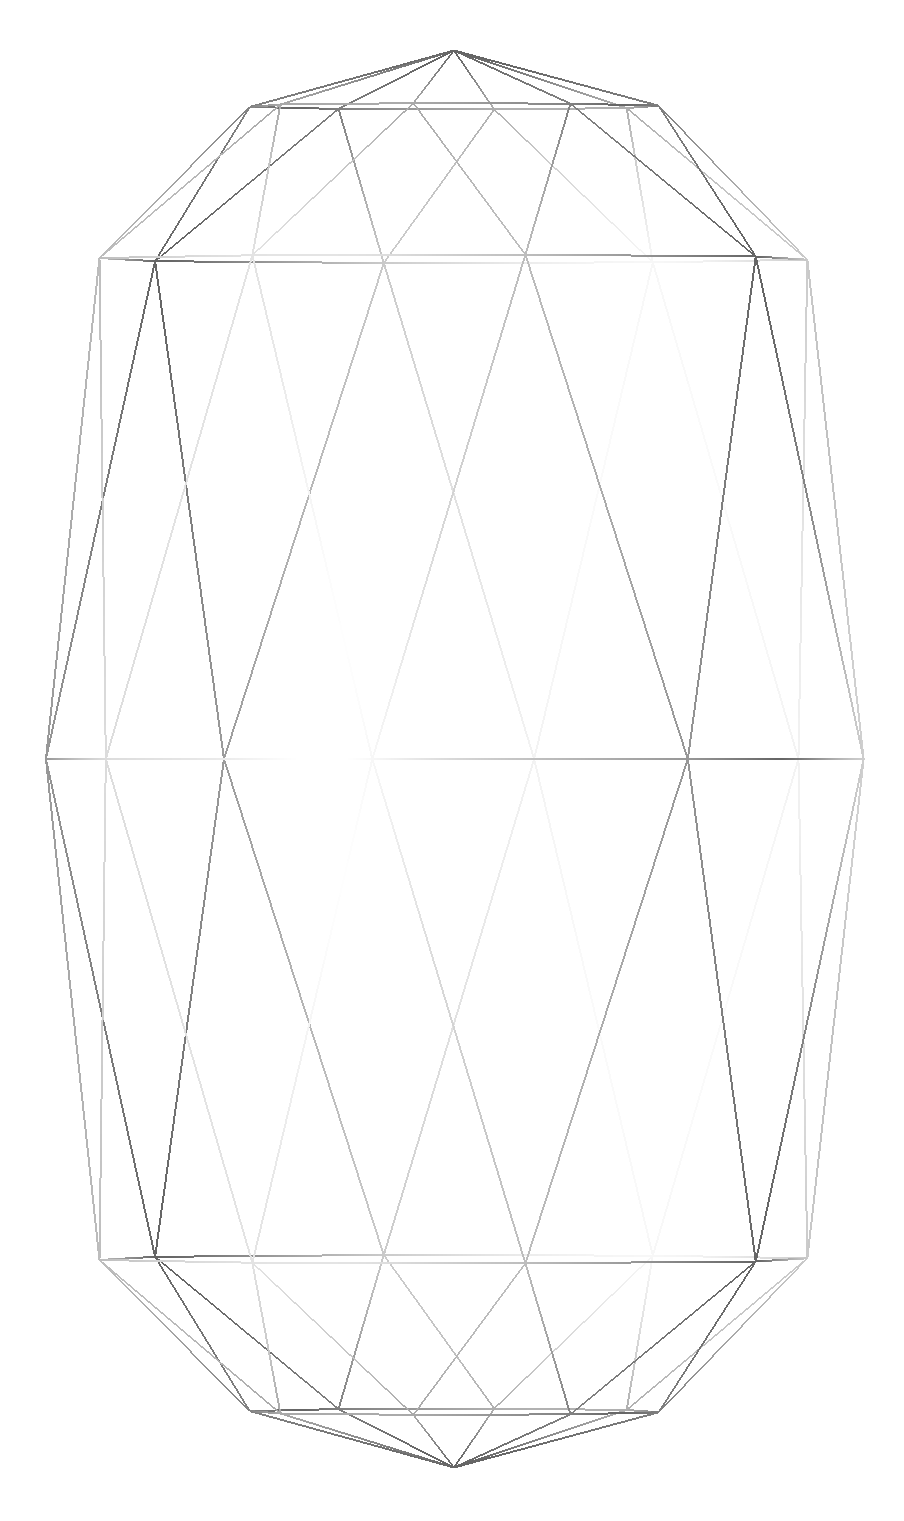
\includegraphics[width=\textwidth]{assets/images/shapes/sphero_bug/low_2}
      \caption{\makefirstuc{Low mesh density.}}
      \label{fig:sphero_bug_low_2}
    \end{subfigure}
        \begin{subfigure}{0.3\textwidth}
      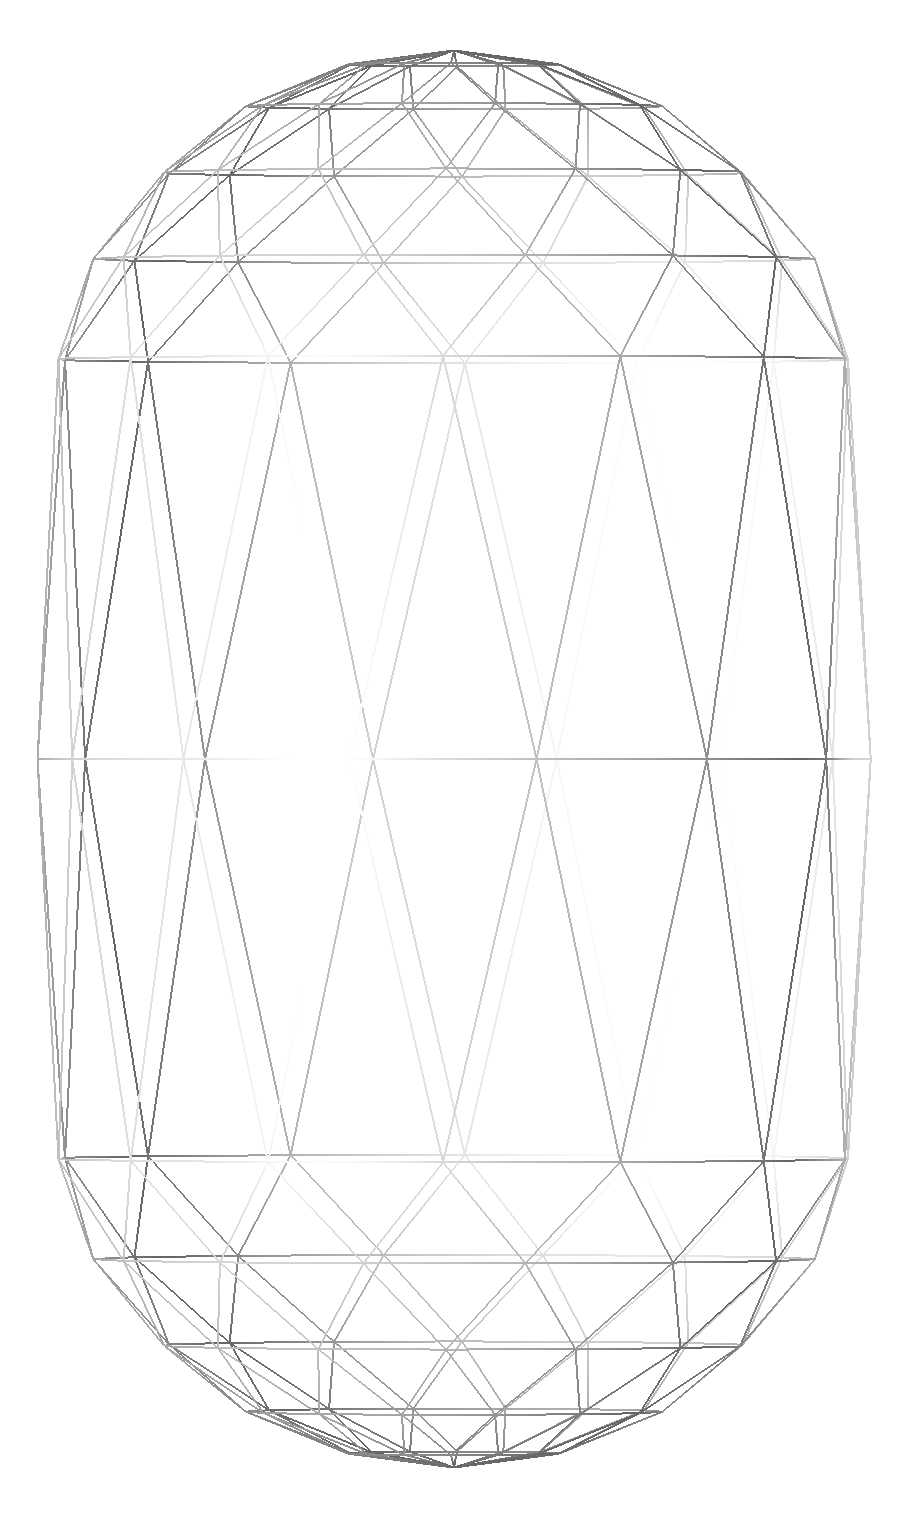
\includegraphics[width=\textwidth]{assets/images/shapes/sphero_bug/med_2}
      \caption{\makefirstuc{Medium mesh density.}}
      \label{fig:sphero_bug_med_2}
    \end{subfigure}
        \begin{subfigure}{0.3\textwidth}
      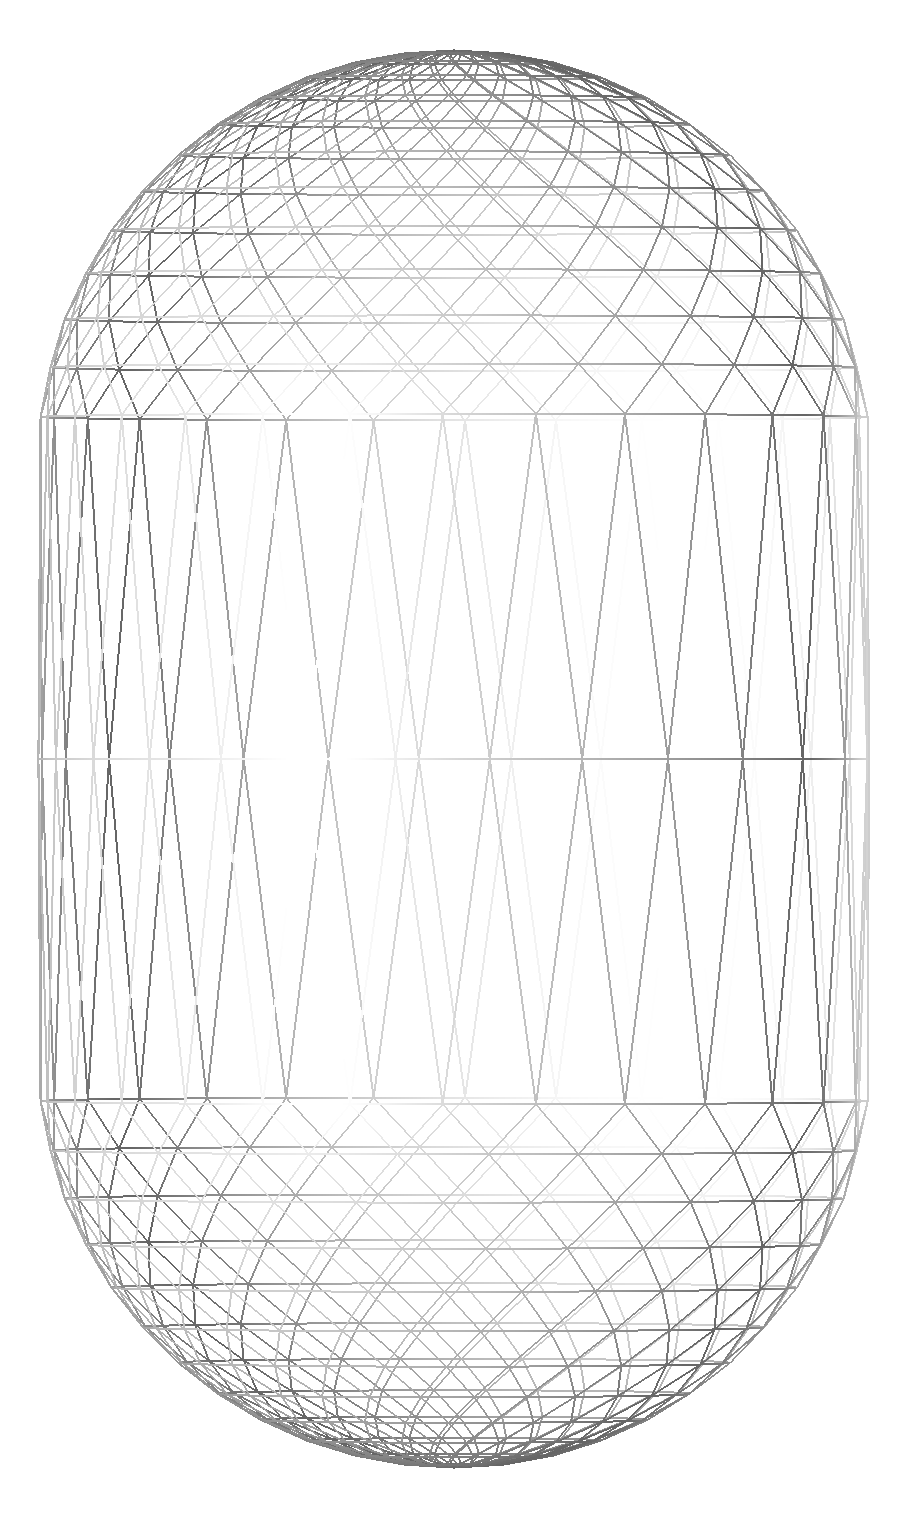
\includegraphics[width=\textwidth]{assets/images/shapes/sphero_bug/high_2}
      \caption{\makefirstuc{High mesh density.}}
      \label{fig:sphero_bug_high_2}
    \end{subfigure}
  \end{center}
  \caption{Initial spherocylinder implementation. Visible tapering can be observed, particularly with low mesh density.}
  \label{fig:sphero_bug}
\end{figure}
Unfortunately, this process produced visually unsatisfying results with the sides of the spherocylinder visibly tapering, particularly with low detail meshes. This can be seen in \cref{fig:sphero_bug}. After producing the biconvex lens (\cref{biconvex_section}), an alternate, much simpler solution became apparent which avoided this issue.
\paragraph{Second Attempt}

A spherocylinder can also be considered a special case of the biconvex lens. A biconvex lens with no separation and aperture angle $\frac{\pi}{2}$ produces a sphere with the given radius $r$. Increasing the separation parameter causes the two hemispheres to move apart such that a spherocylinder is produced. The spherocylinder can therefore simply be considered a special case of the biconvex lens with aperture angle $\frac{\pi}{2}$, and can be implemented entirely through class inheritance as shown:
\begin{lstlisting}
//Spherocylinder mesh generator
export class Spherocylinder extends BiconvexLens {
    constructor(radius: number, length: number) {
        super(radius, Math.PI / 2, length);
    }
}
\end{lstlisting}
This produced the result shown in \cref{fig:spherocylinder_shape}.
\shapefigure{spherocylinder}{spherocylinder}

\subsection{WebMGA 3.0 Bugs}
TODO

\section{File types}
\subsection{WebMGA 2.0 Implementation}
WebMGA 2.0 supports only its own JSON-based file format as defined in CITEORIGINALDISSERTATION. This could prove an obstacle to users since, in practice, different formats are output when running molecular dynamics simulations (CITE!!).

\subsection{WebMGA 2.0 Bugs}
TODO

\subsection{WebMGA 3.0 Implementation}
WebMGA 3.0 implements two new file formats for defining molecular configurations as defined below.
\subsubsection{LAMMPS Format (.cnf)}
LAMMPS is a molecular dynamics simulator typically used on highly parallel computers\cite{thompson2022lammps}. It uses a specifically designed file format to represent molecular configurations to allow the highest possible performance while preserving some amount of human readability.

\cref{tab:lammps_format} shows the structure of a file of this format. Rows represent lines in the file. Each value is represented by a signed float of format $-1.000000 $, where digits before the decimal are omitted if not present. Values are separated by spaces, padded to align decimal points.

For WebMGA 3.0, a parser script was written in JavaScript which builds a WebMGA JSON configuration from the ``.cnf'' file provided. Specifically, a unit box is constructed from $(lx, ly, lz)$, and molecule positions and orientations are obtained from corresponding pairs of $(rx,ry,rz)$ and $(ex,ey,ez)$ for some molecule id. All other parameters are dropped since they aren't used by WebMGA. Molecules are ordered in an array according to their id.
\begin{table}
  \begin{center}
  \begin{adjustbox}{width=\textwidth}
    \begin{tabular}{|c|c|c|c|c|c|c|c|c|c|c|c|c|}
      \hline
      Molecule count & & & & & & & & & & & &\\
      \hline
      Unit box X length ($lx$) & & & & & & & & & & & &\\
      \hline
      Unit box Y length ($ly$) & & & & & & & & & & & &\\
      \hline
      Unit box Z length ($lz$) & & & & & & & & & & & &\\
      \hline
      Not used & Not used & & & & & & & & & & &\\
      \hline
      Position ($rx$) & Position ($ry$) & Position ($rz$) & Velocity ($vx$) & Velocity ($vy$) & Velocity ($vz$) & Orientation ($ex$) & Orientation ($ey$) & Orientation ($ez$) & Orientational velocity ($ux$) & Orientational velocity ($uy$) & Orientational velocity ($uz$) & Molecule ID\\
      \hline
      \vdots & \vdots & \vdots & \vdots & \vdots & \vdots & \vdots & \vdots & \vdots & \vdots & \vdots & \vdots & \vdots \\
       \hline
    \end{tabular}
  \end{adjustbox}
  \end{center}
  \caption{LAMMPS format molecule configuration}
  \label{tab:lammps_format}
\end{table}

\subsubsection{Cinacchi Format (.qmga)}
TODO WRITE THIS
TODO CHECK LETTERS USED FOR ROTATION ETC

See \cref{tab:cinacchi_format} for the structure of a file of this format. Rows represent lines in the file. Each value is represented by a signed float of format $-1.00000000$, where digits before the decimal are omitted if not present. Values are separated by spaces, padded to align decimal points.

For WebMGA 3.0, a parser script was written in JavaScript which builds a WebMGA JSON configuration from the ``.qmga'' file provided. Specifically, a unit box is constructed from $(lx, ly, lz)$, and molecule positions and orientations are obtained from corresponding pairs of $(rx,ry,rz)$ and $(ex,ey,ez)$. The shape parameter is dropped since molecule shape is not defined by the file. Molecules are ordered in an array as they are encountered.
\begin{table}
  \begin{center}
  \begin{adjustbox}{width=\textwidth}
    \begin{tabular}{|c|c|c|c|c|c|c|}
      \hline
       Unit box X half length ($lx/2$) & Unit box Y half length ($ly/2$) & Unit box Z half length ($lz/2$) & & & &\\
       \hline
       Shape parameter & Position X ($rx$) & Position Y ($ry$) & Position Z ($rz$) & Orientation X ($ex$) & Orientation Y ($ey$) & Orientation Z ($ez$)\\
       \hline
       \vdots & \vdots & \vdots & \vdots & \vdots & \vdots & \vdots \\
       \hline
    \end{tabular}
  \end{adjustbox}
  \end{center}
  \caption{Cinacchi format molecule configuration}
  \label{tab:cinacchi_format}
\end{table}

\subsection{WebMGA 3.0 Bugs}
WebMGA ignores the shape parameter from the ``.qmga'' format configuration. Since some shapes in WebMGA require multiple parameters, and the shape to use is not defined within the file, I could not see a sensible way to automate applying this. The user must manually enter this value after selecting a molecule shape in the ``Models'' menu. This is not ideal since a user should expect their configuration to appear correctly as soon as they load the file.

\section{Periodic Repetition (TODO RENAME THIS?}
\subsection{Improvement Goals}
A description for periodic boundary conditions is given in \cref{pbc_explain} regarding how a small simulation box simulates a subset of an infinite lattice. It may be useful to visualise a larger subset of this infinite lattice by repeating the simulation box a number of times. Additionally, the capability of repeating a smaller system is useful for producing a realistic, much larger configuration for testing the performance of WebMGA with increased molecule counts due to the lack of availability of real test configurations of such sizes.

\subsection{WebMGA 3.0 Implementation}
A few modifications needed to be made to implement this feature.

First, the ``reference'' tab in the side menu was modified to include inputs for the repeat count in the `x' `y' and `z' directions. With a value of zero, there should be only a single instance of the configuration along the corresponding axis. Setting to one adds a repeat in the positive and negative direction along the axis, with bounding box faces touching (i.e. with a value of 0, there will be 1 instance of the configuration, with 1 there will be 3 instances, 2 there will be 5 instances etc.). When multiple directions have a value larger than 0, the configurations are repeated such that a single large box is produced (i.e. it is ensured there are no gaps, for example a configuration of $(1,1,1)$ will give a box of dimensions $3\times 3\times 3$ with $27$ total instances of the initial configuration).

Repetition of the configuration was implemented by changing TODO FINISH THIS

\begin{figure}
  \begin{center}
    \begin{subfigure}{0.3\textwidth}
      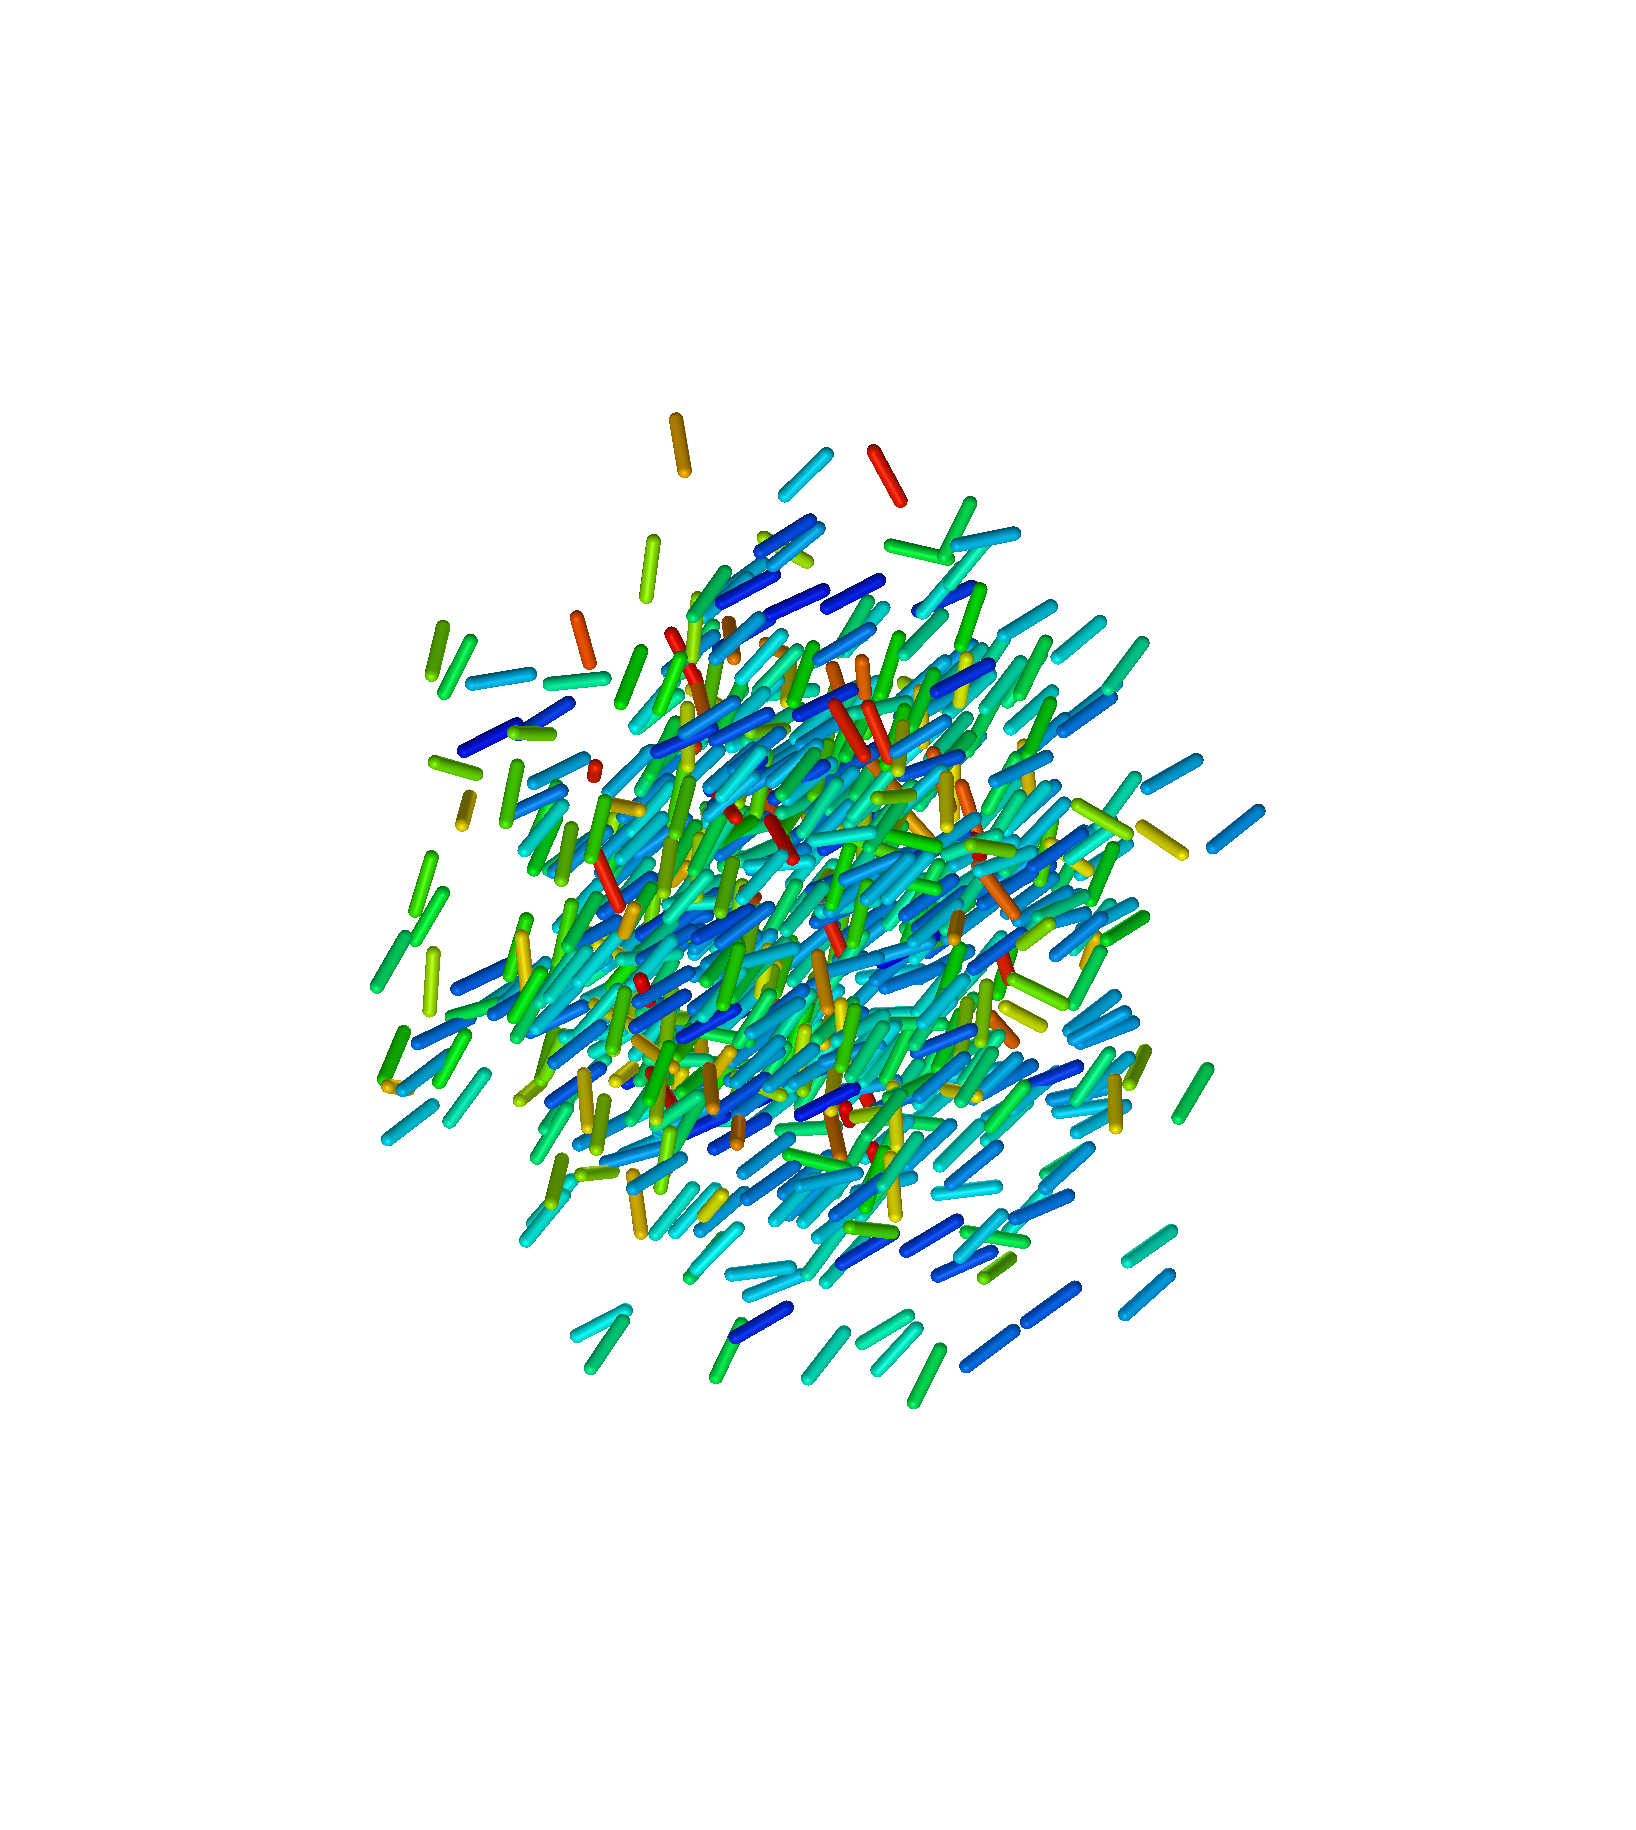
\includegraphics[width=\textwidth]{assets/images/periodic/1}
      \caption{$(0,0,0)$}
      \label{fig:periodic_1}
    \end{subfigure}
        \begin{subfigure}{0.3\textwidth}
      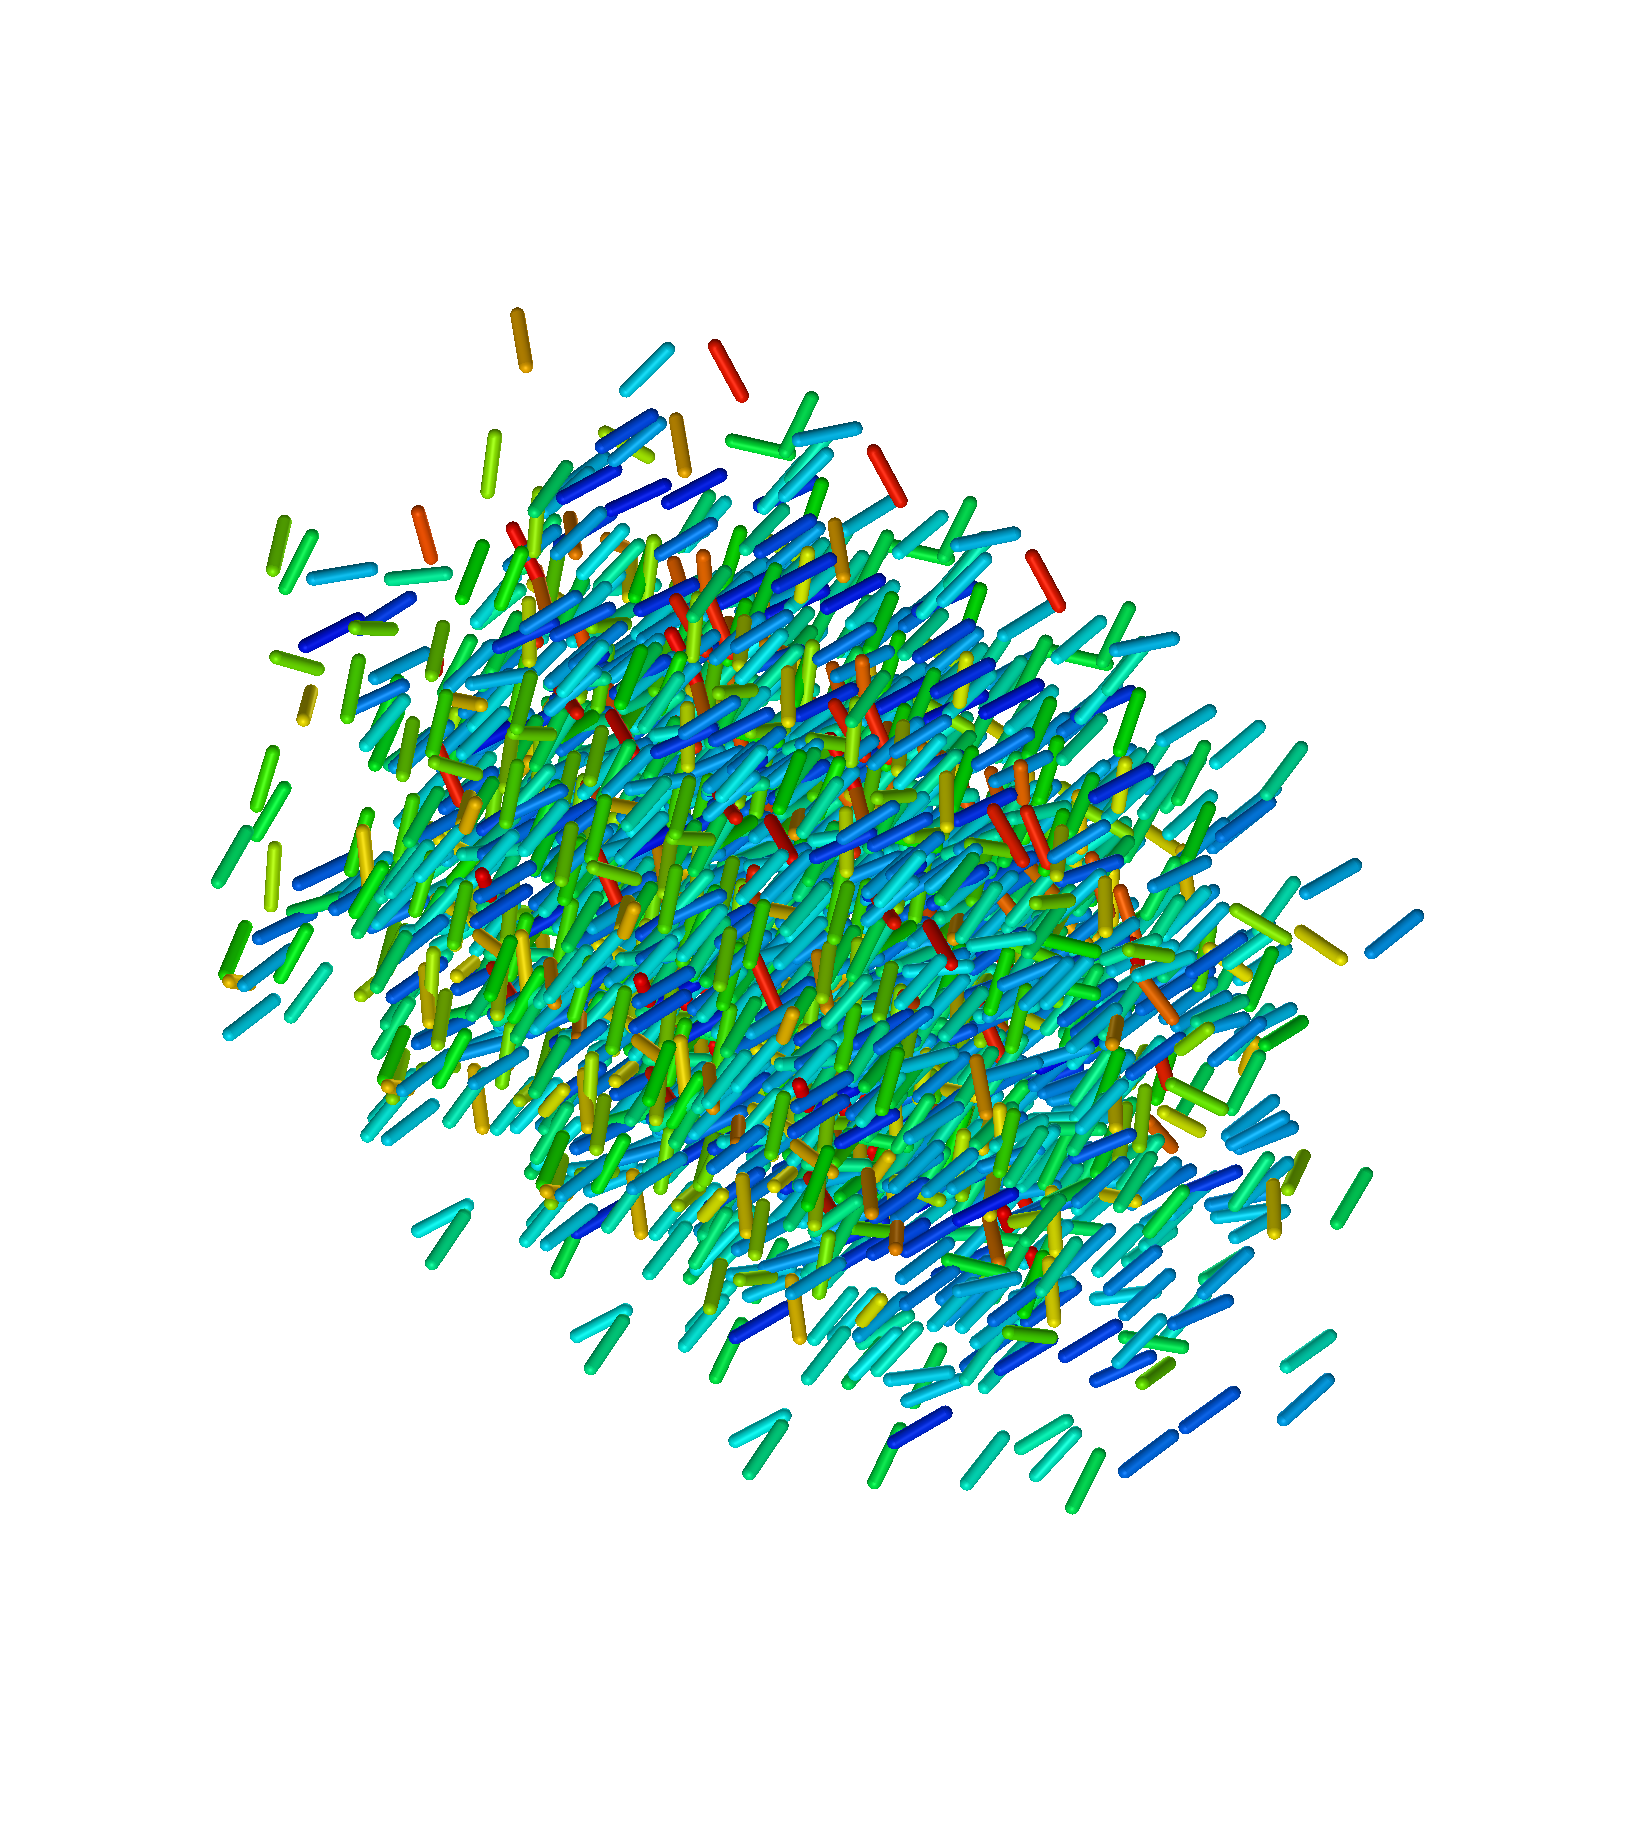
\includegraphics[width=\textwidth]{assets/images/periodic/2}
      \caption{$(1,0,0)$}
      \label{fig:periodic_2}
    \end{subfigure}
        \begin{subfigure}{0.3\textwidth}
      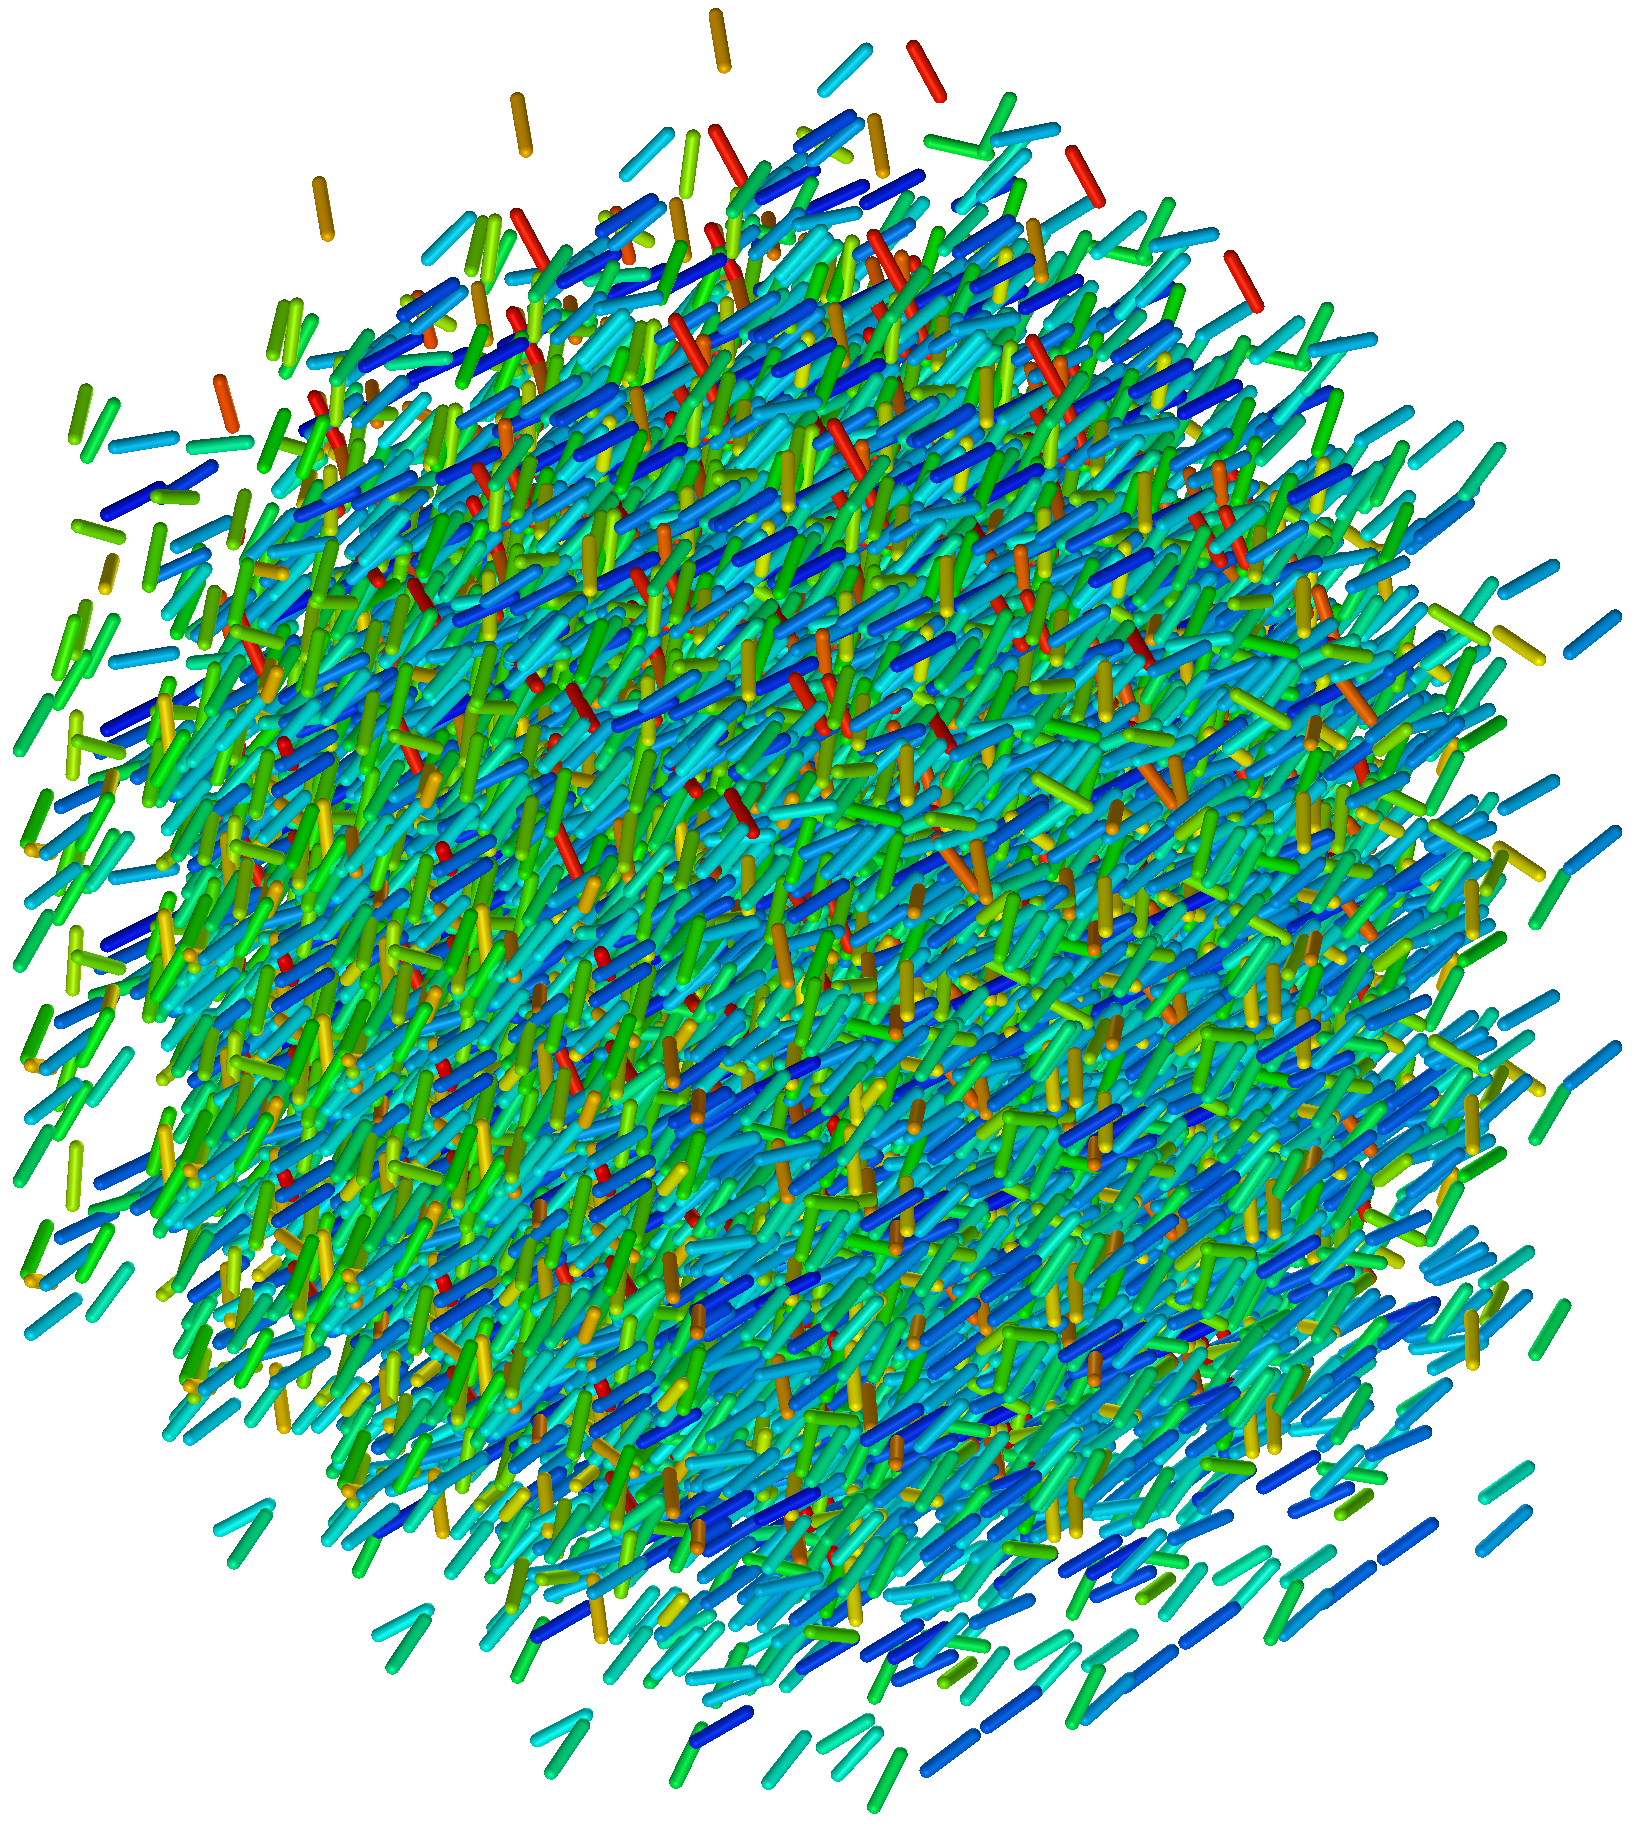
\includegraphics[width=\textwidth]{assets/images/periodic/3}
      \caption{$(1,1,1)$}
      \label{fig:periodic_3}
    \end{subfigure}
  \end{center}
  \caption{Demonstration of periodic repetition of a configuration, labelled with repetition parameter of format $(x, y, z)$.}
  \label{fig:periodic}
\end{figure}

\subsection{WebMGA 3.0 Bugs}
TODO

\section{Optimisations}
\subsection{WebMGA 2.0 Implementation}
TODO

\subsection{WebMGA 2.0 Bugs}
TODO

\subsection{WebMGA 3.0 Implementation}
\subsubsection{Discrete Levels of Detail}
\begin{figure}
  \begin{center}
    \begin{subfigure}{0.3\textwidth}
      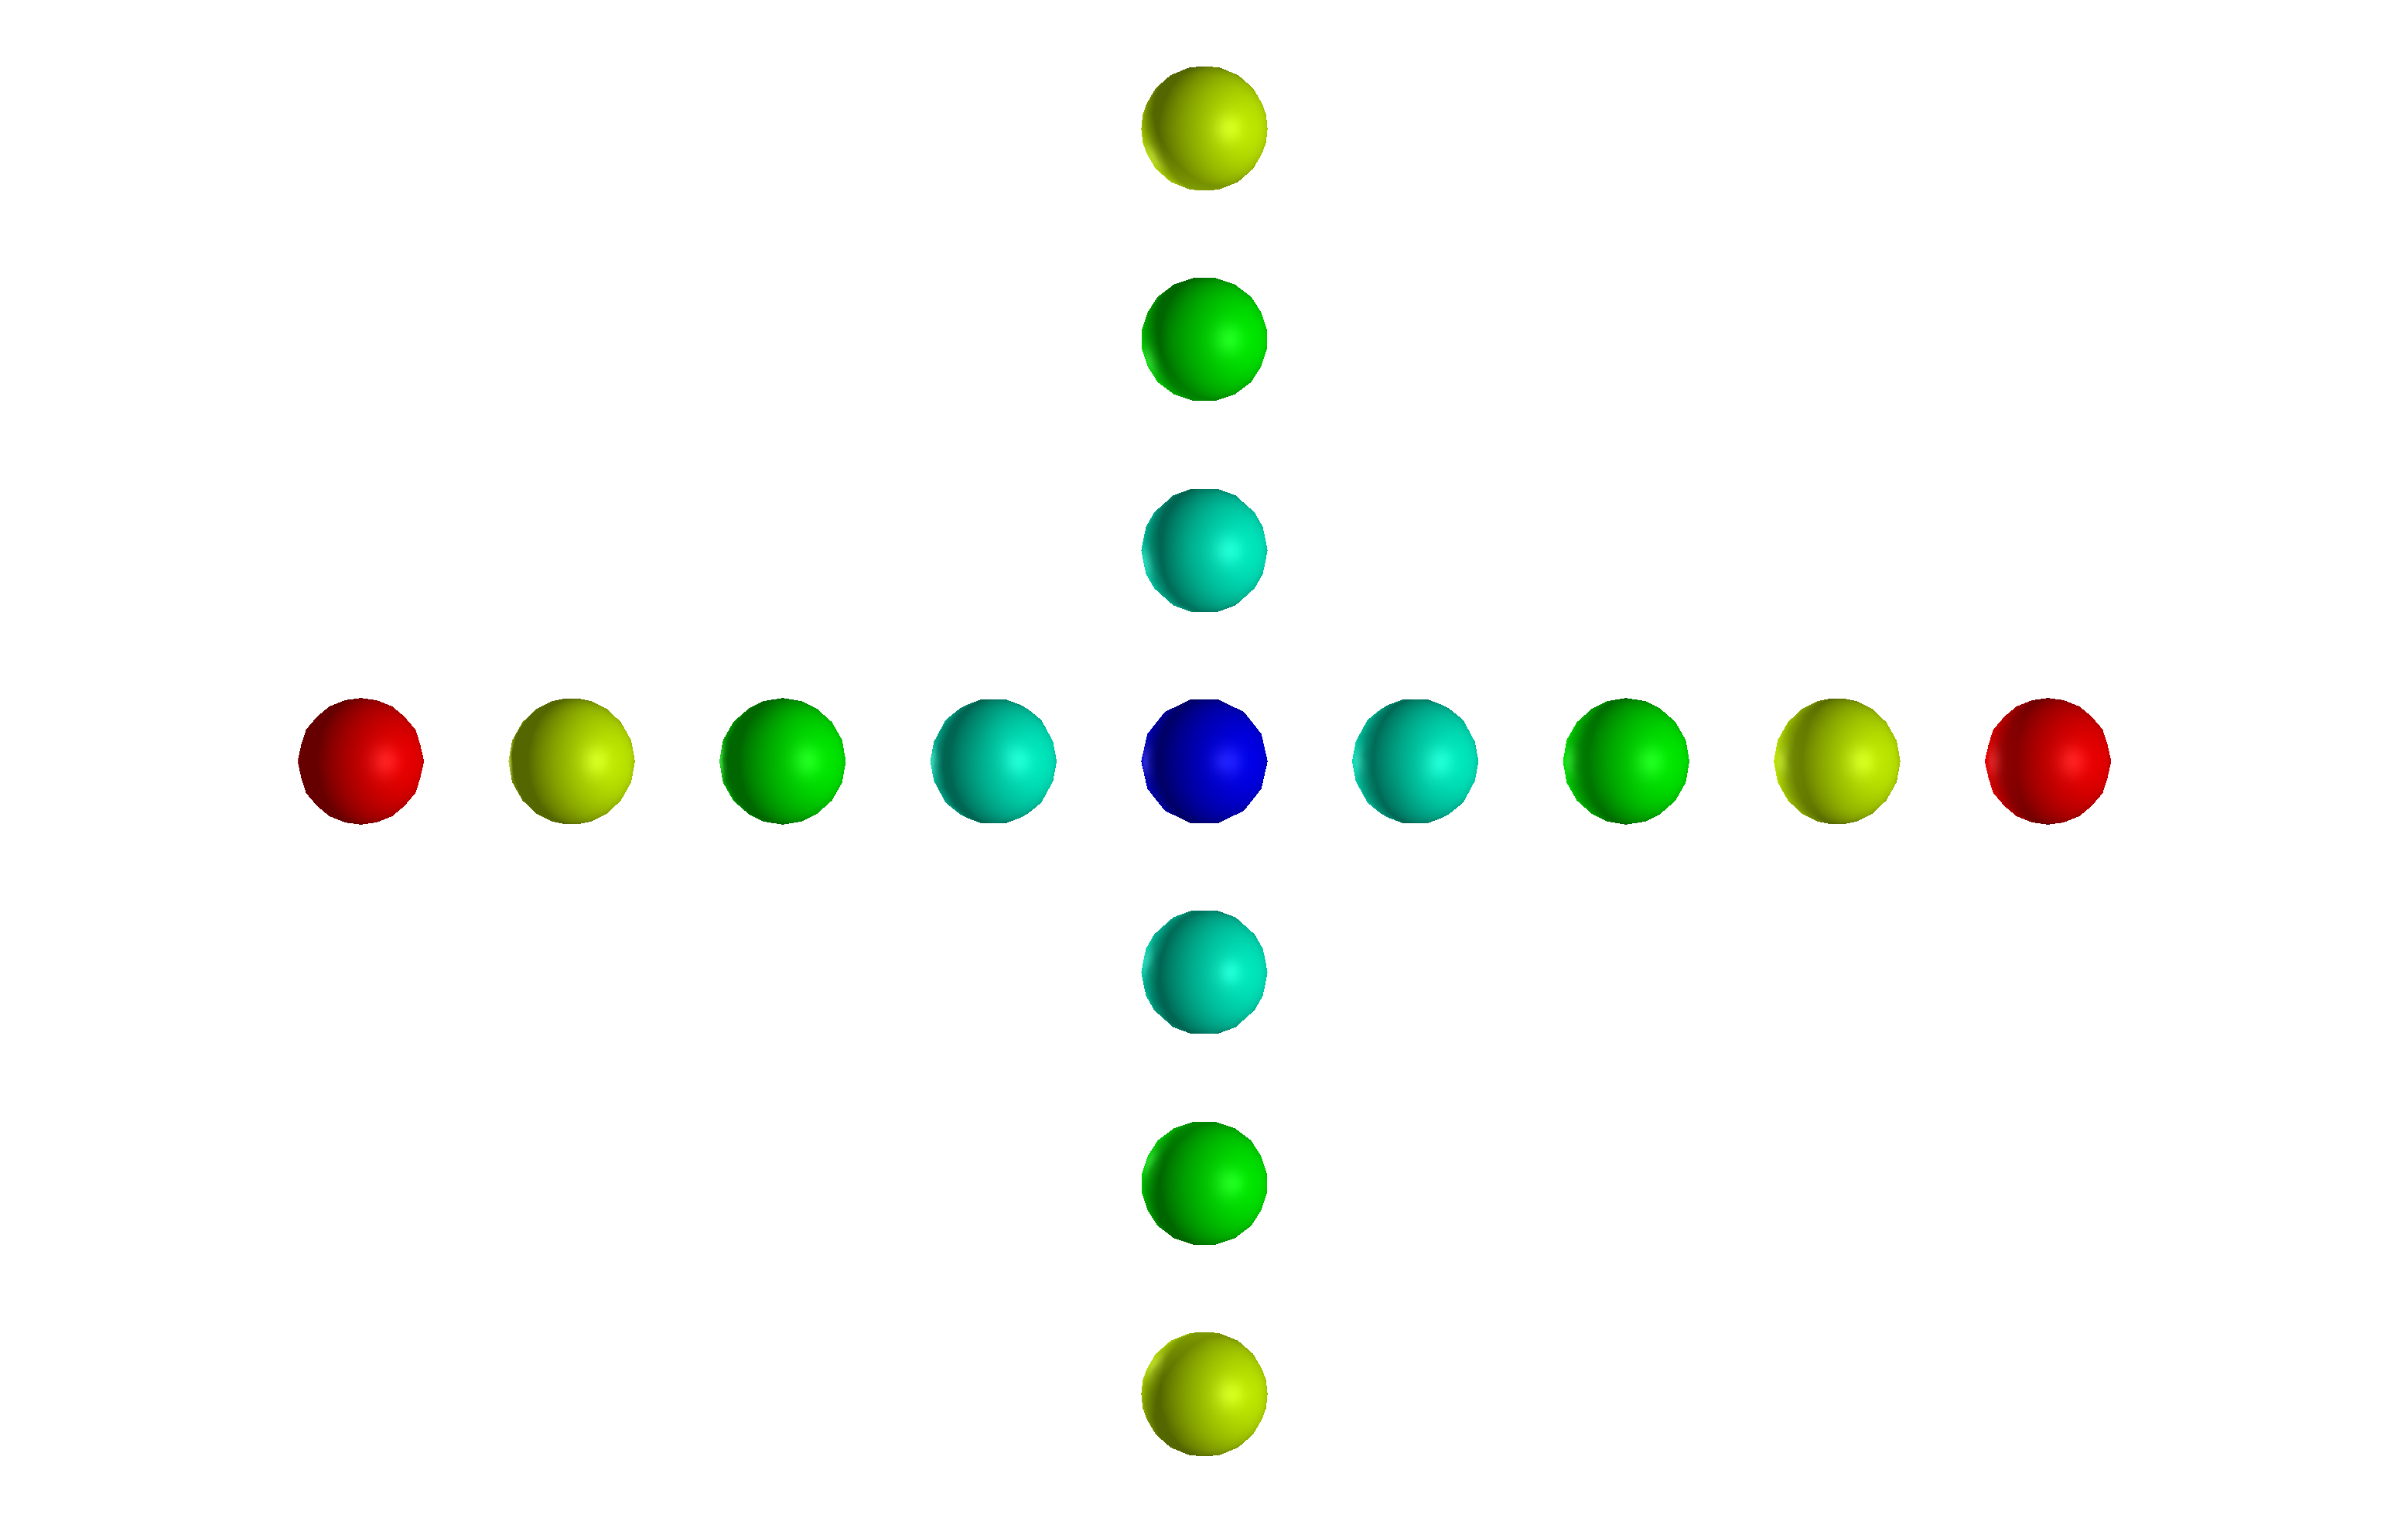
\includegraphics[width=\textwidth]{assets/images/lod/1}
      \caption{Low detail.}
      \label{fig:lod_1}
    \end{subfigure}
    \begin{subfigure}{0.3\textwidth}
      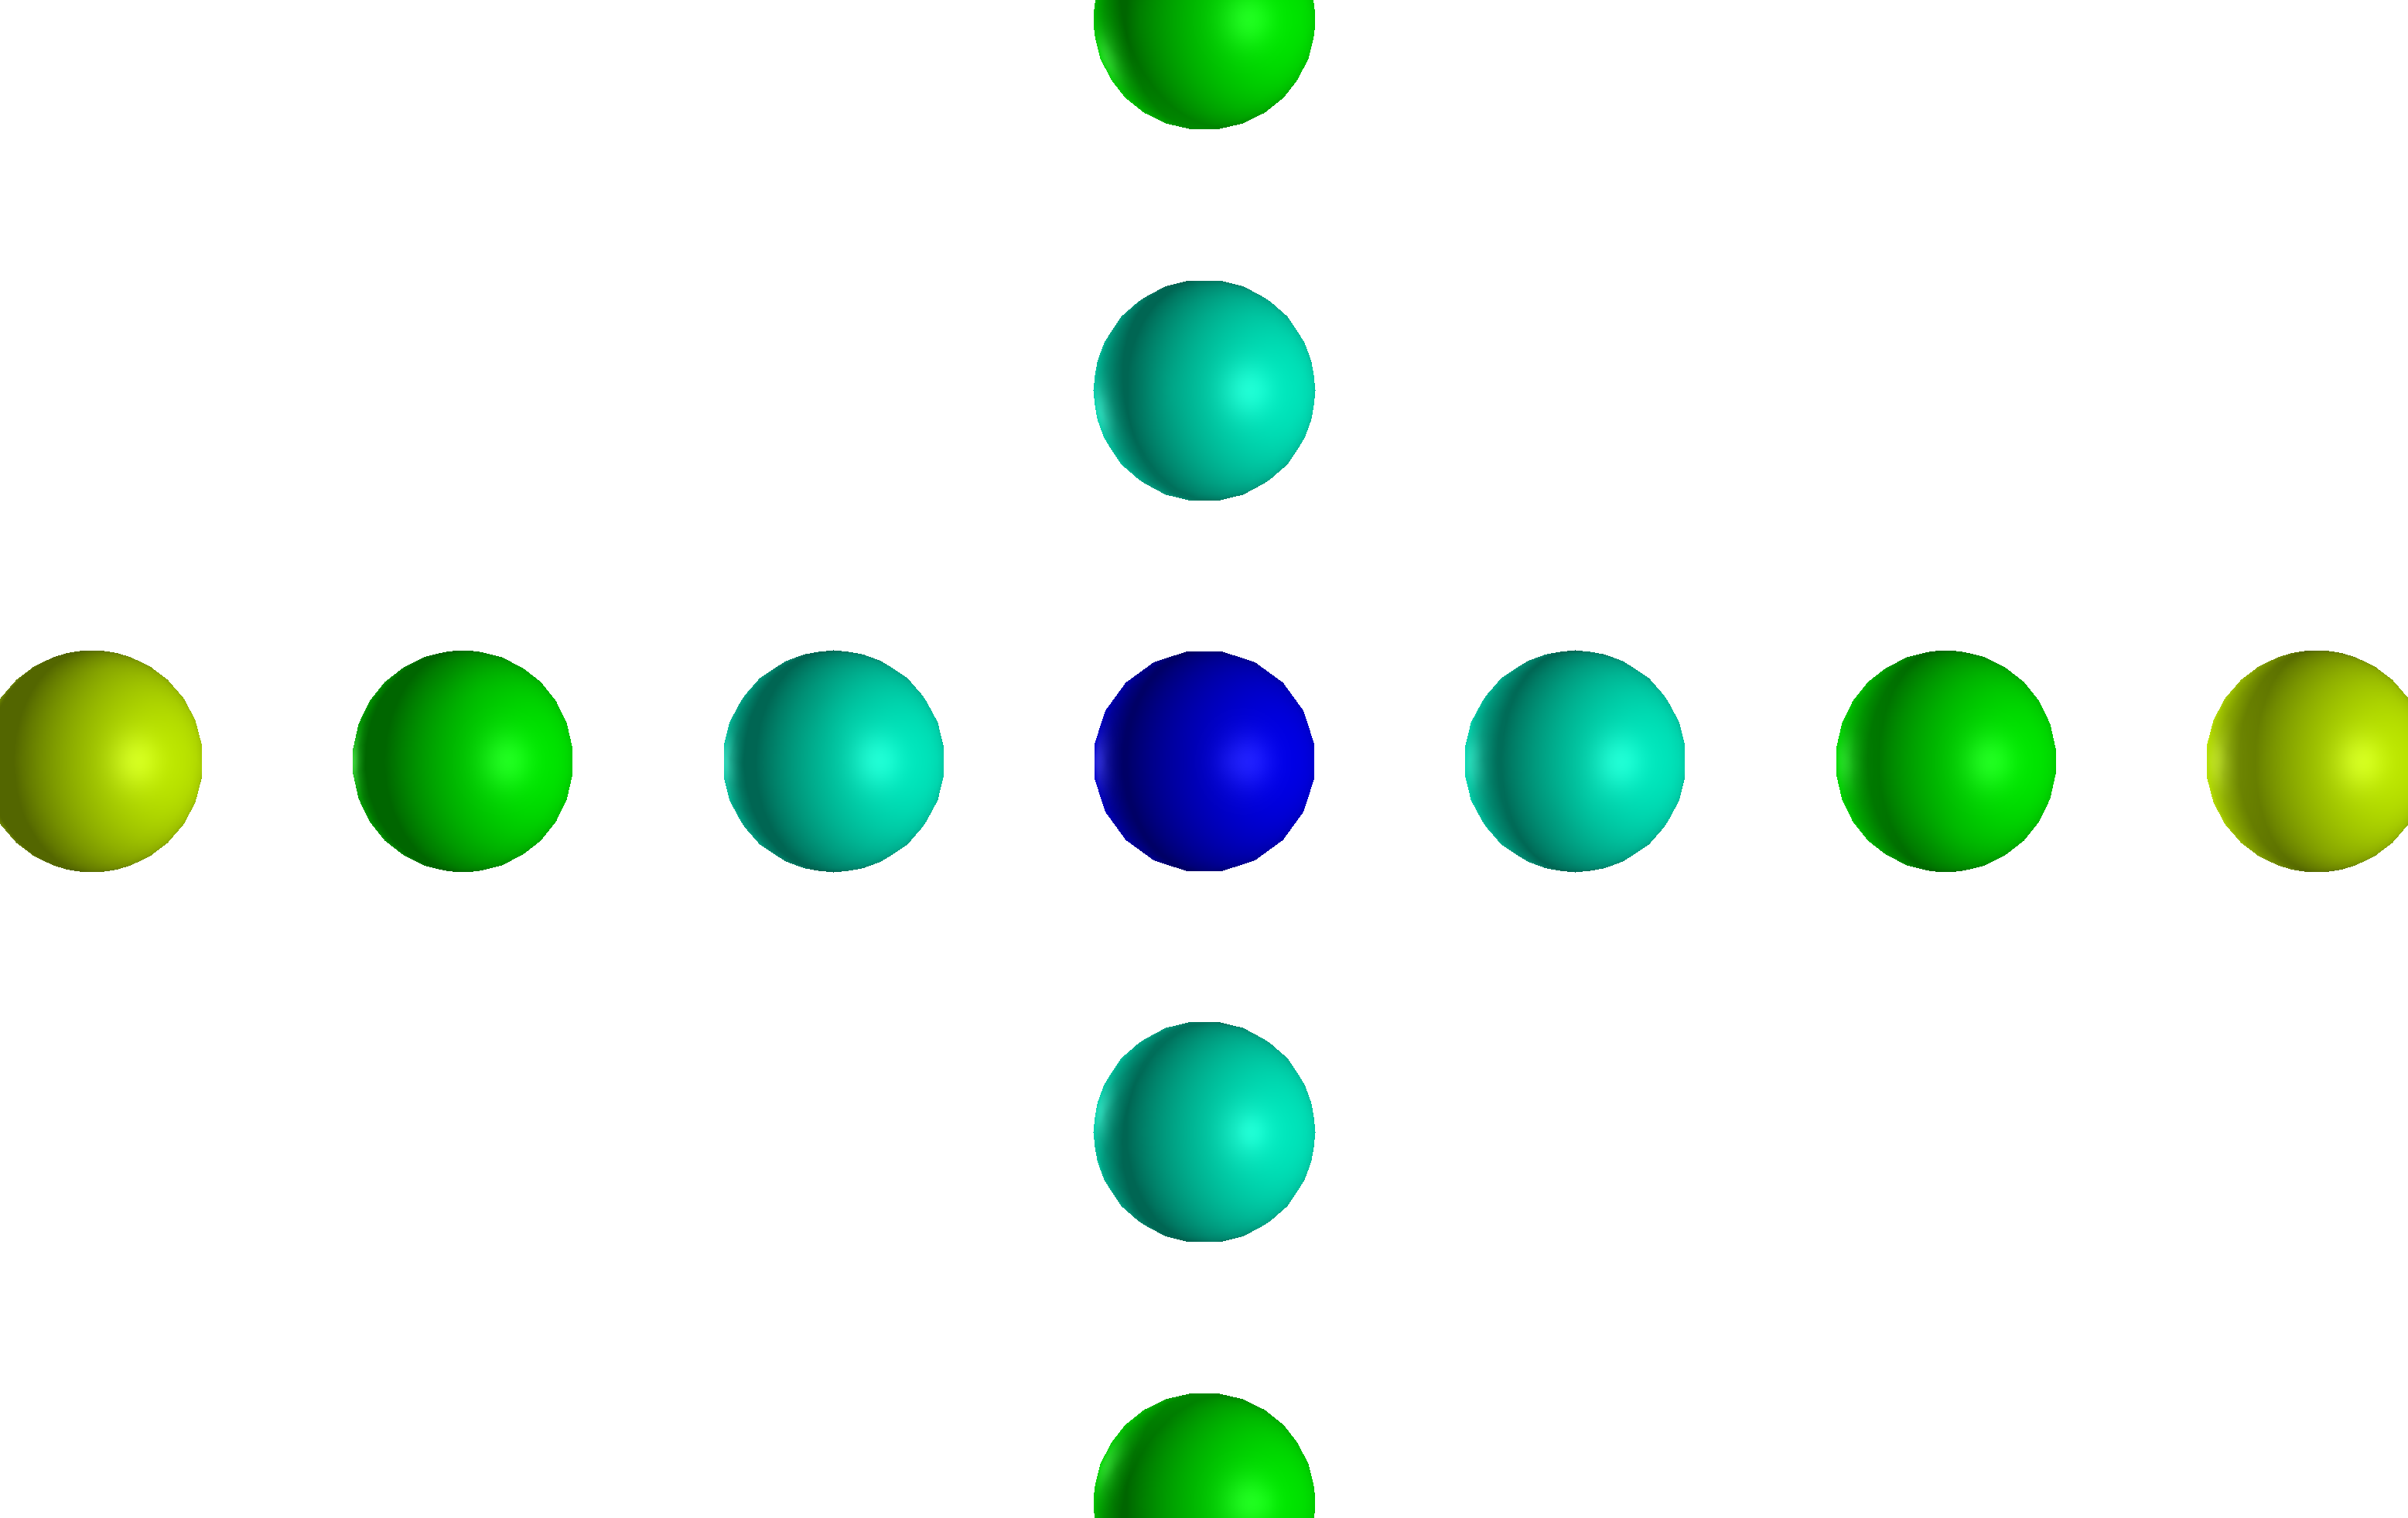
\includegraphics[width=\textwidth]{assets/images/lod/2}
      \caption{Medium detail.}
      \label{fig:lod_2}
    \end{subfigure}
    \begin{subfigure}{0.3\textwidth}
      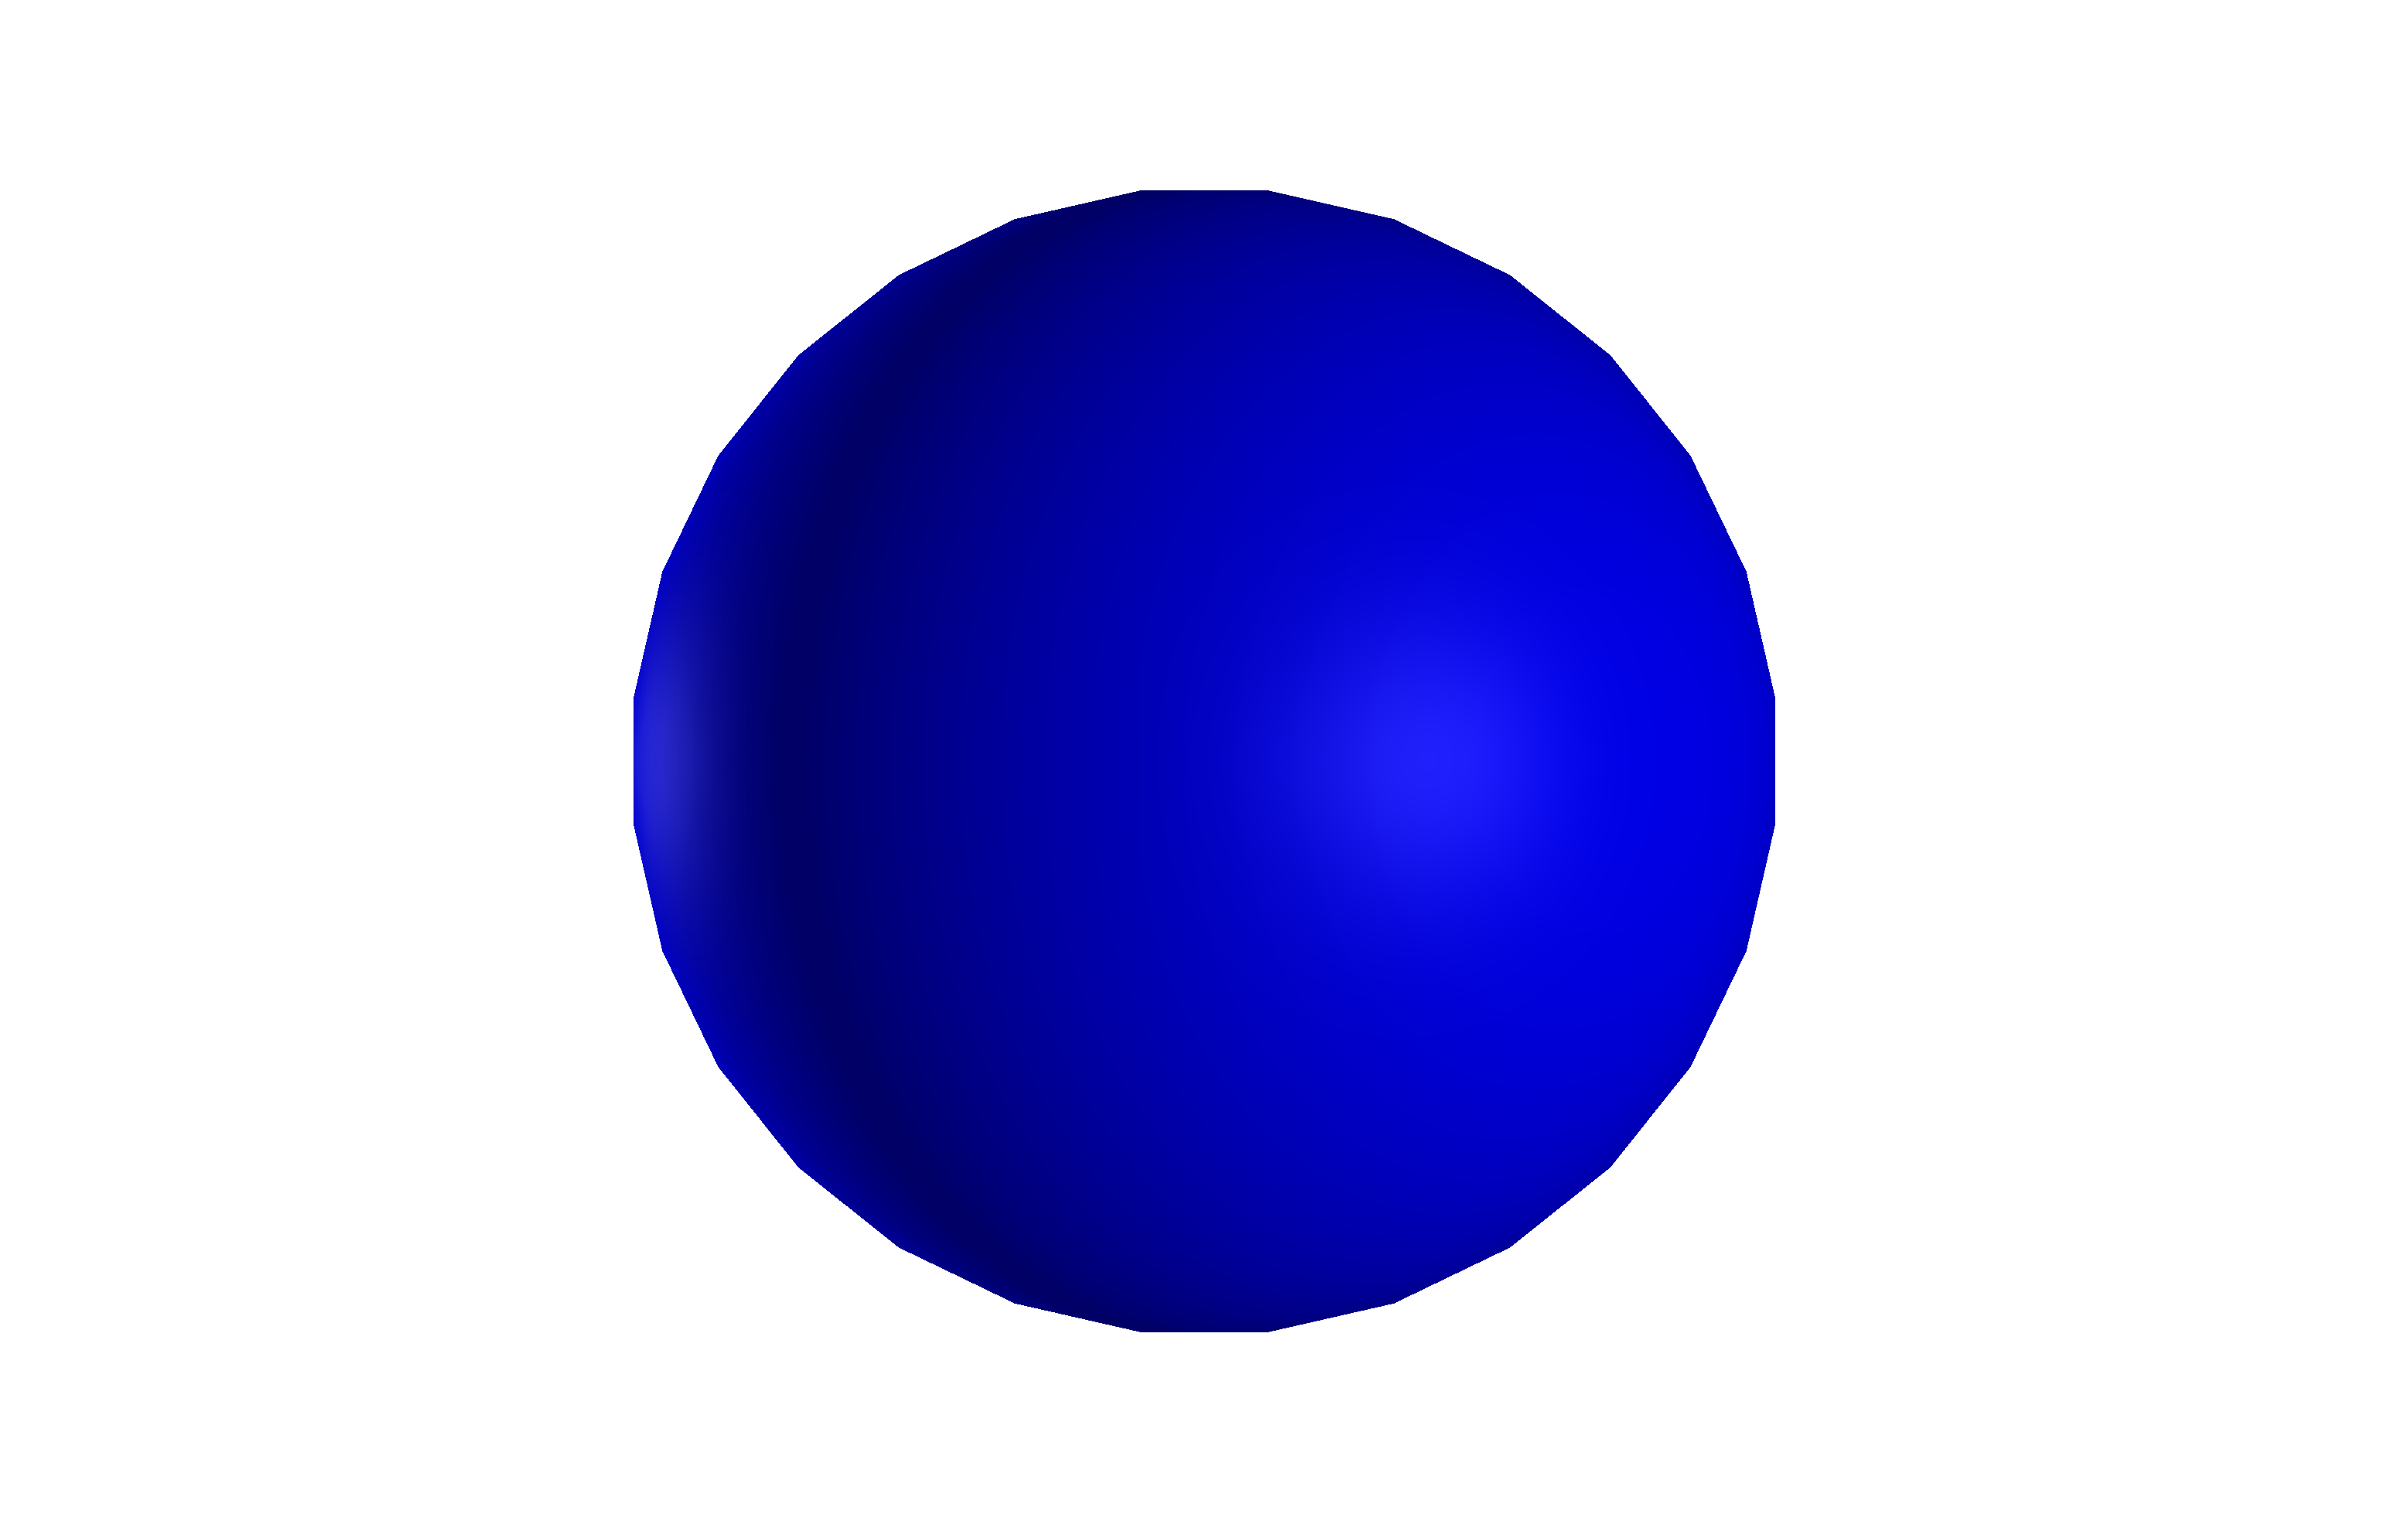
\includegraphics[width=\textwidth]{assets/images/lod/3}
      \caption{Full detail.}
      \label{fig:lod_3}
    \end{subfigure}
    
    \begin{subfigure}{0.3\textwidth}
      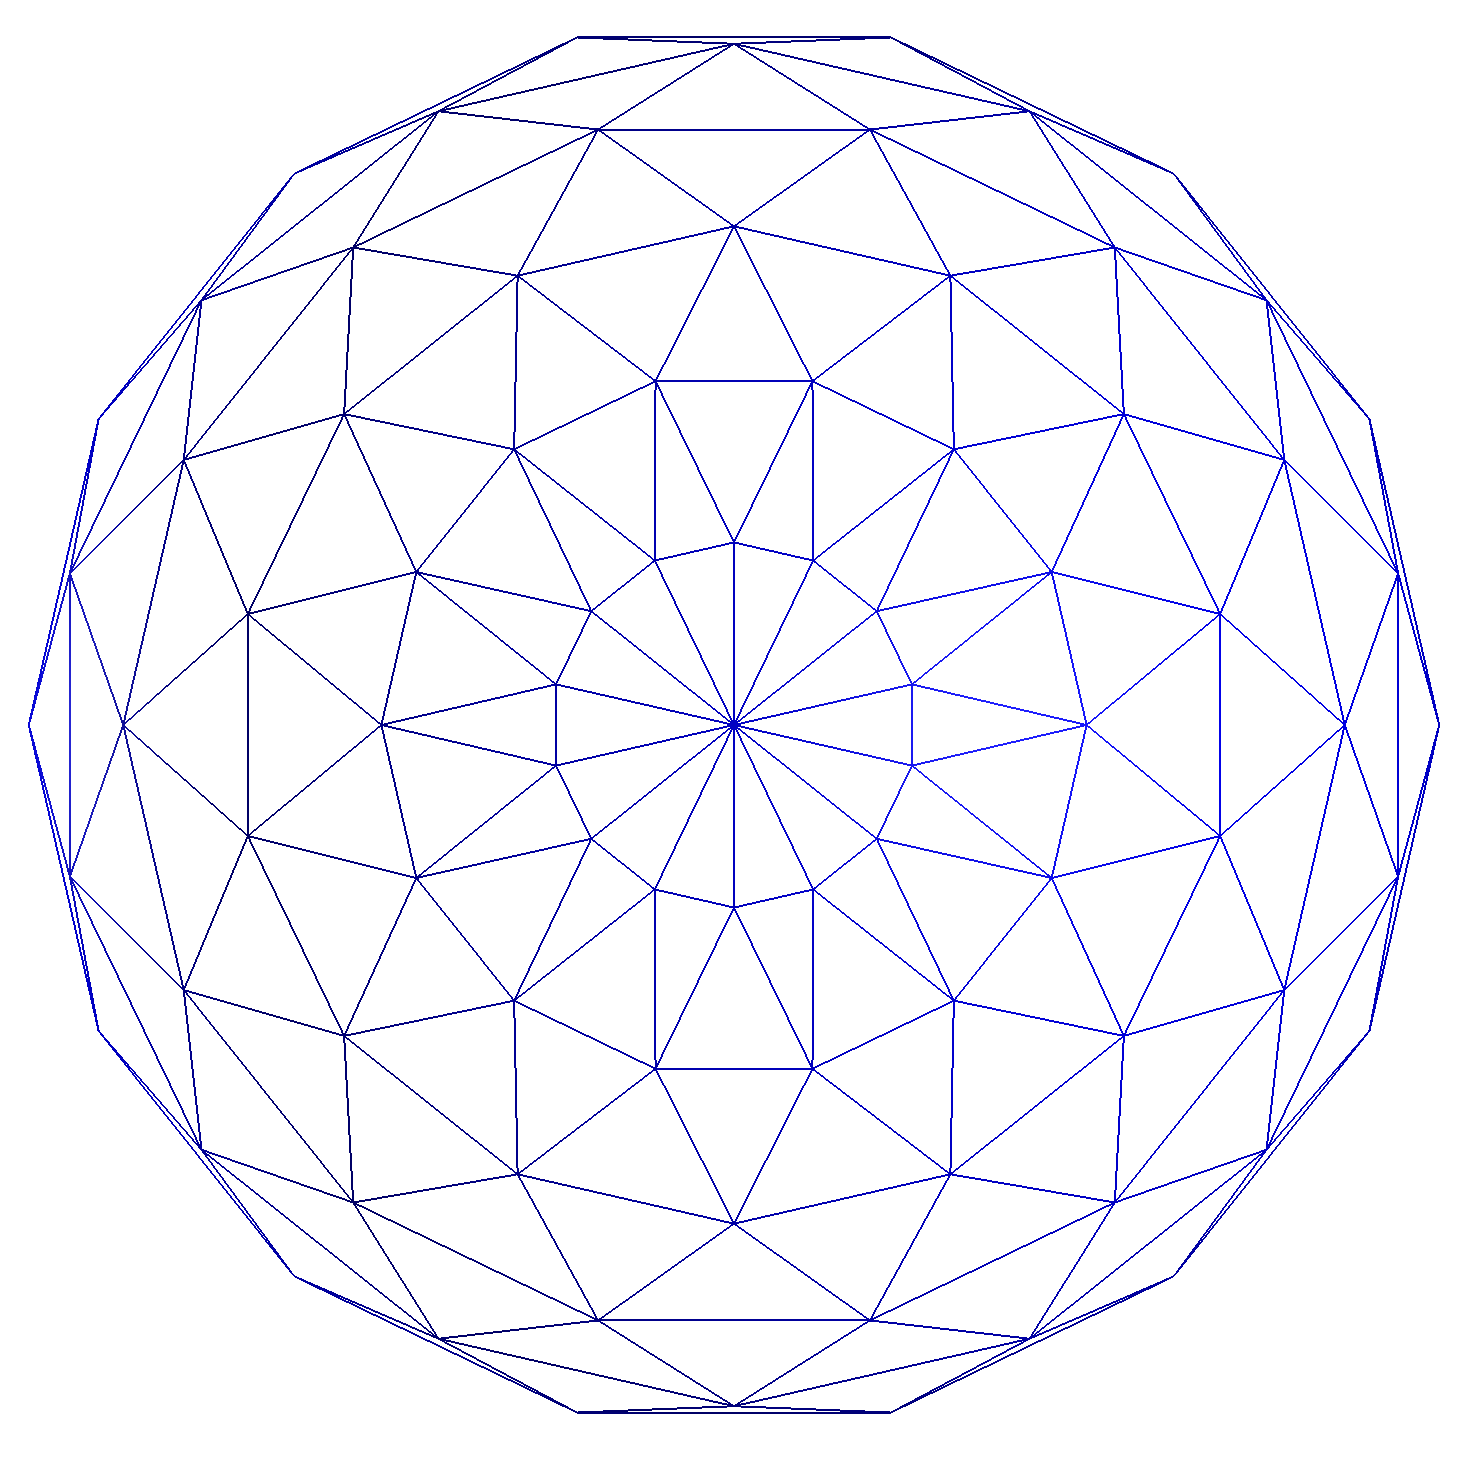
\includegraphics[width=\textwidth]{assets/images/lod/1_w}
      \caption{Low detail.}
      \label{fig:lod_1_w}
    \end{subfigure}
    \begin{subfigure}{0.3\textwidth}
      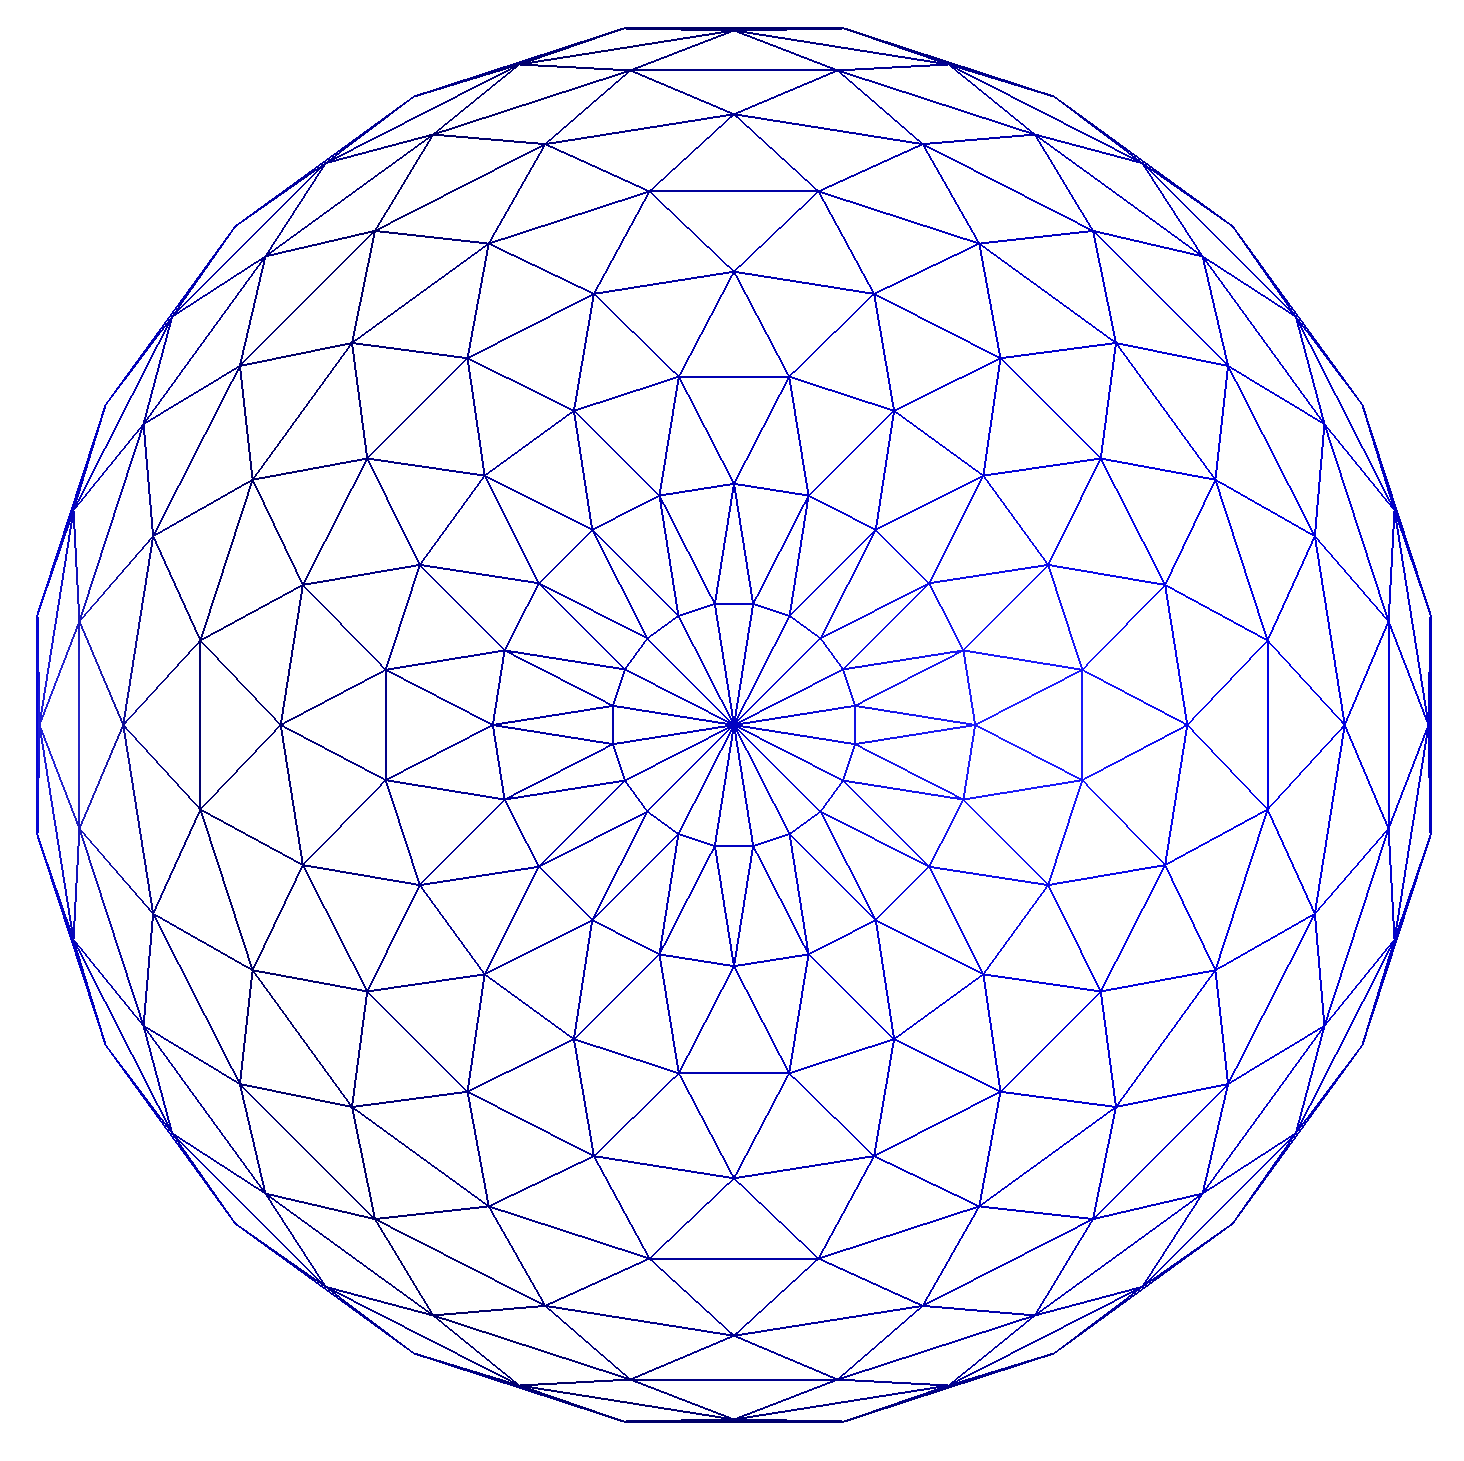
\includegraphics[width=\textwidth]{assets/images/lod/2_w}
      \caption{Medium detail.}
      \label{fig:lod_2_w}
    \end{subfigure}
    \begin{subfigure}{0.3\textwidth}
      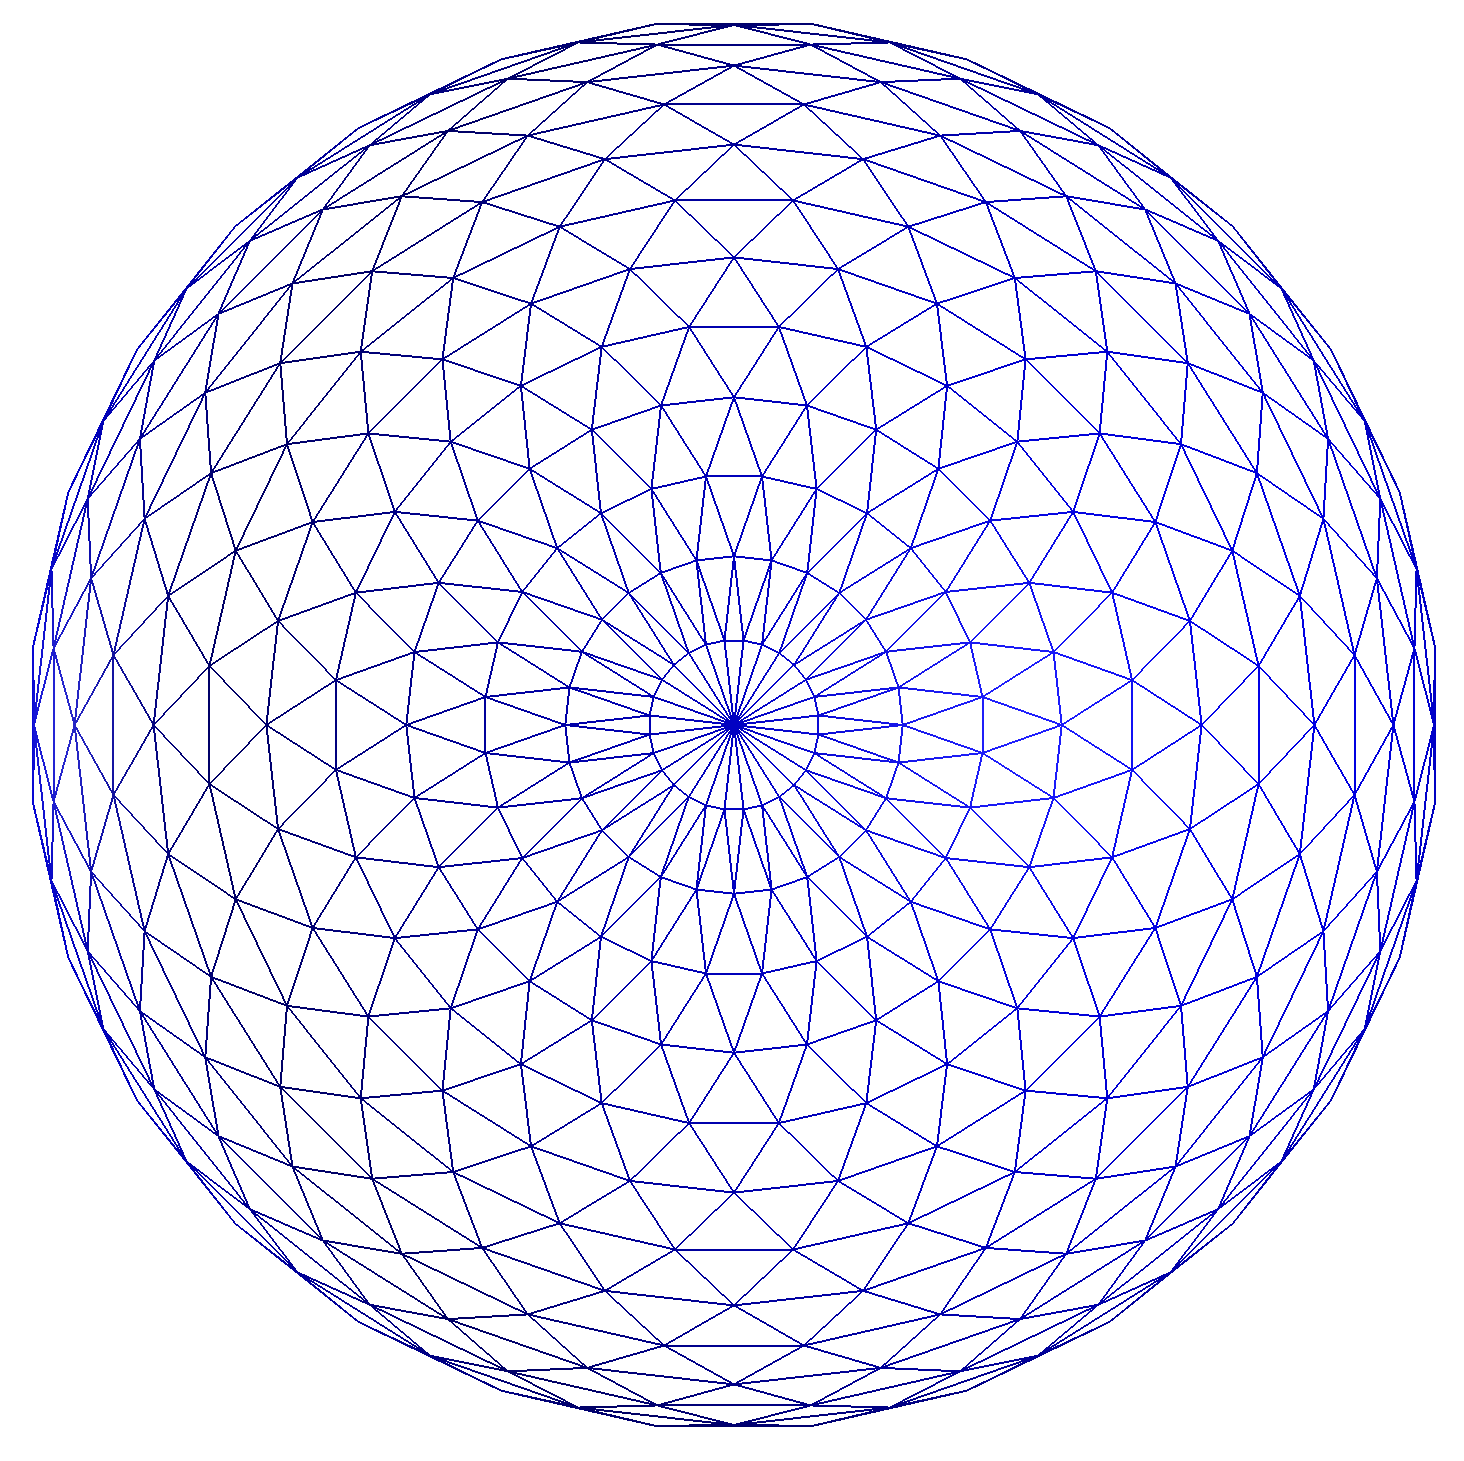
\includegraphics[width=\textwidth]{assets/images/lod/3_w}
      \caption{Full detail.}
      \label{fig:lod_3_w}
    \end{subfigure}
  \end{center}
  \caption{Model complexity is decreased at subjectively chosen camera distance thresholds with minimal visible loss in quality.}
  \label{fig:lod_distances}
\end{figure}

\begin{figure}
  \begin{center}
    \begin{subfigure}{\textwidth}
      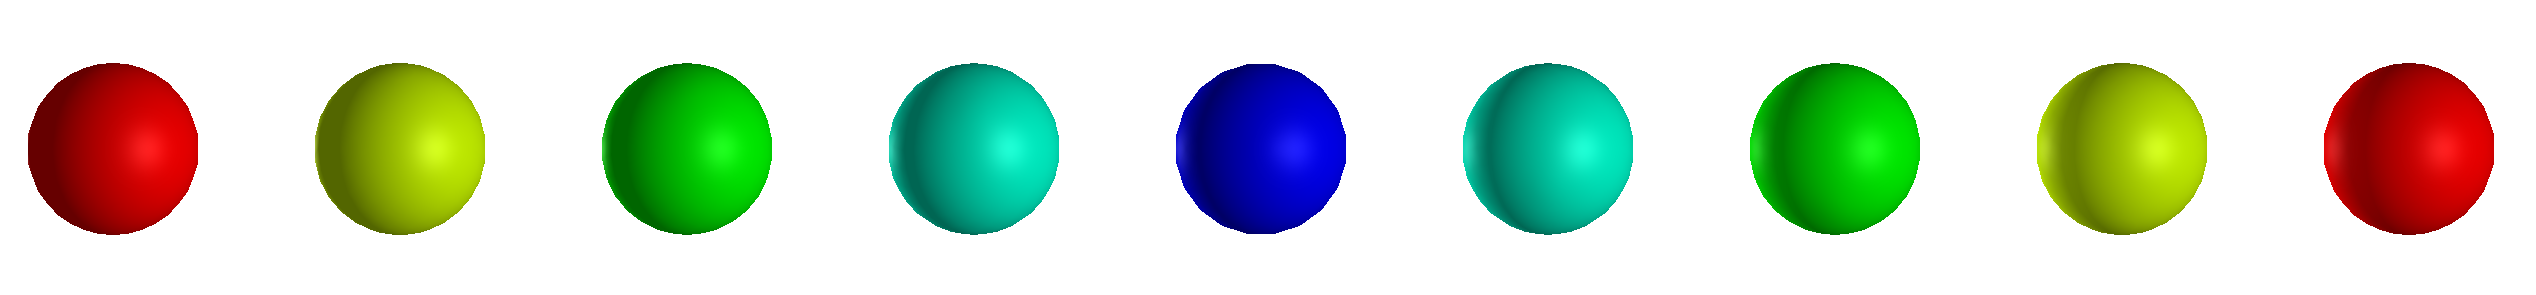
\includegraphics[width=\textwidth]{assets/images/lod/a}
      \caption{At a similar distance, all objects are identical.}
      \label{fig:lod_a}
    \end{subfigure}
    \begin{subfigure}{\textwidth}
      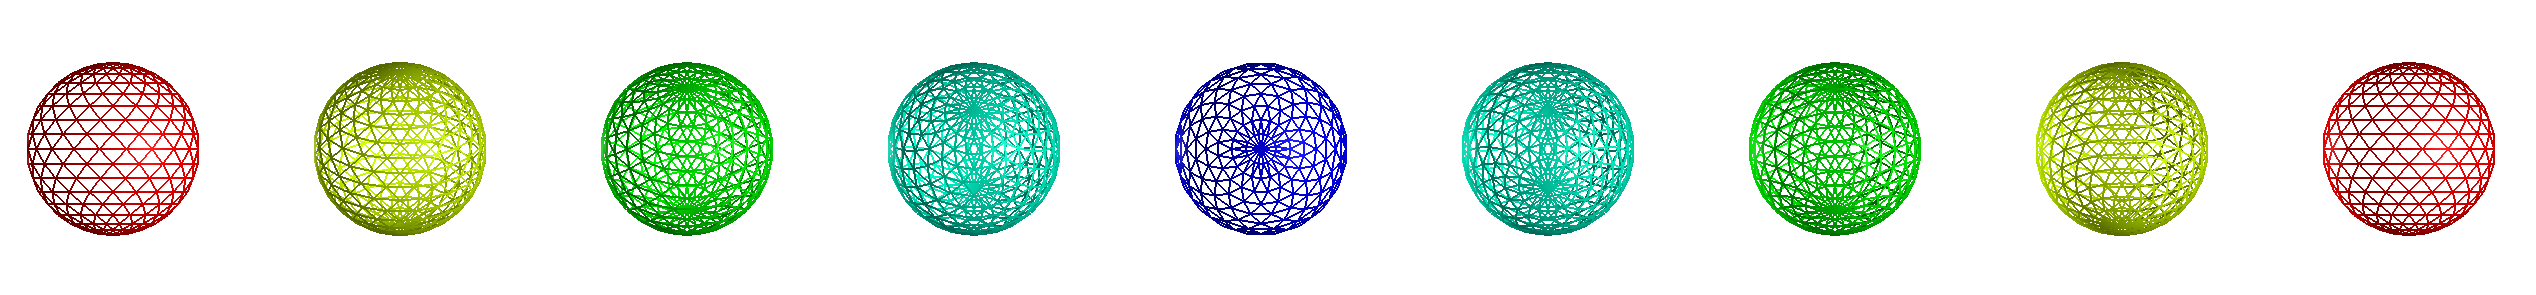
\includegraphics[width=\textwidth]{assets/images/lod/a_w}
      \caption{At a similar distance, all meshes are identical.}
      \label{fig:lod_a_w}
    \end{subfigure}
    \begin{subfigure}{\textwidth}
      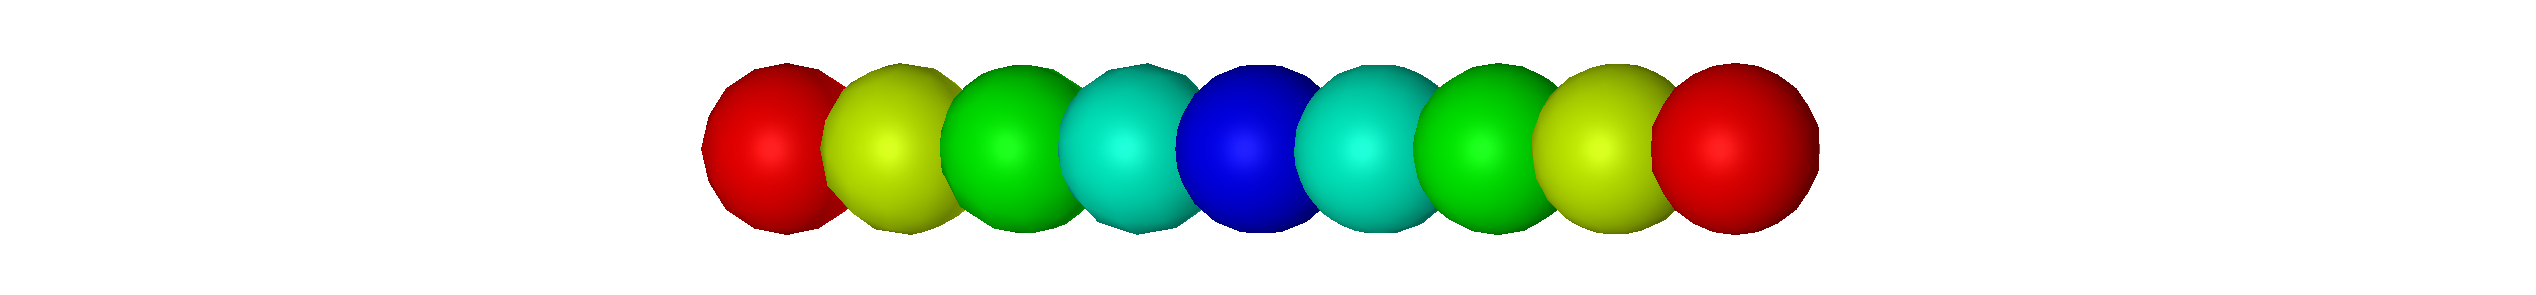
\includegraphics[width=\textwidth]{assets/images/lod/b}
      \caption{Further spheres have a minor decrease in visible quality.}
      \label{fig:lod_b}
    \end{subfigure}
    \begin{subfigure}{\textwidth}
      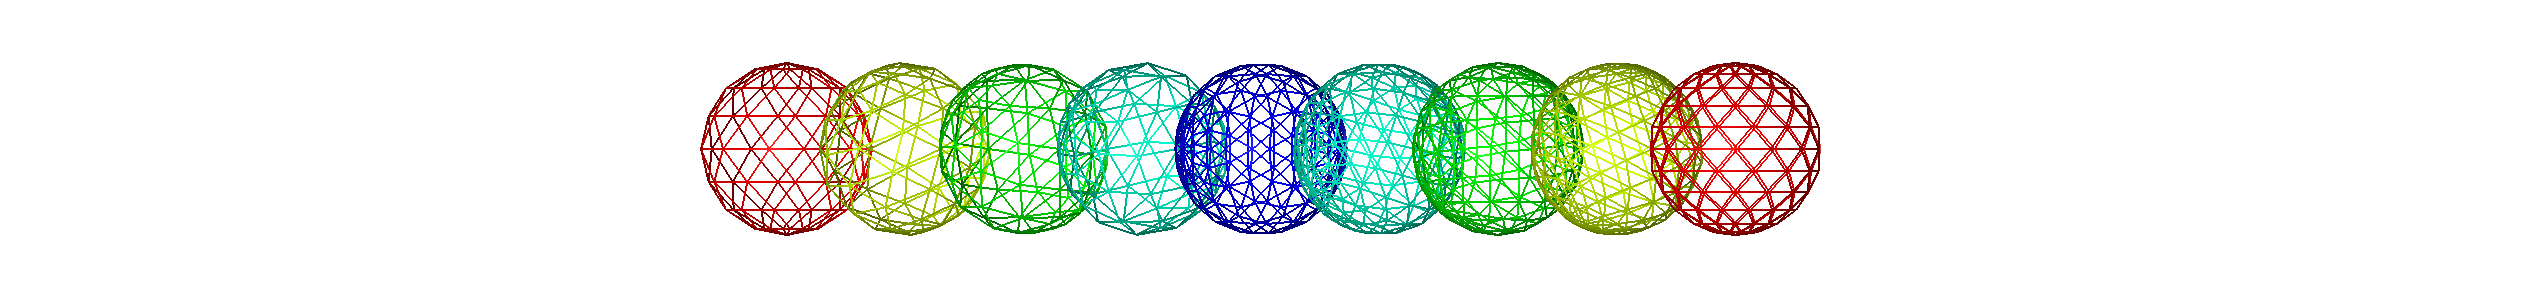
\includegraphics[width=\textwidth]{assets/images/lod/b_w}
      \caption{Further spheres have a minor decrease in triangle density.}
      \label{fig:lod_b_w}
    \end{subfigure}
  \end{center}
  \caption{Demonstration of decreased mesh quality for distant object. ``Level of Detail'' setting has been reduced below default for a more visible geometry reduction.}
  \label{fig:lod_spin}
\end{figure}

Performance analysis for this optimisation is discussed in \cref{lod_analysis_section}.
\subsection{WebMGA 3.0 Bugs}
TODO

\section{Miscellaneous Improvements}


\chapter{Analysis and Testing}
\section{Level of Detail Performance}
\label{lod_analysis_section}
\begin{table}
  \begin{center}
  \begin{adjustbox}{width=\textwidth}
    \begin{tabular}{llrrrr}
    \hline
    \hline
    LOD Enabled & Mesh Quality & Repeats & Distant Framerate (7) & Nearby Framerate (50) & Nearest Framerate (100)\\
    \hline
    True & Highest & $(0,0,0)$ & 64.74 &  33.37 & 35.79 \\
    False & Highest & $(0,0,0)$ & 19.84 & 16.76 & 23.62 \\
    
    True & Default & $(0,0,0)$ & 75.7 & 46.83 & 41.83 \\
    False & Default & $(0,0,0)$ & 74.78 & 35.23 & 36.89 \\
    
    True & Lowest & $(0,0,0)$ & 56.38 & 36.78 & 42.66\\
    False & Lowest & $(0,0,0)$ & 66.34 & 31.75 & 38.28\\
    \hline
    True & Highest & $(1,1,1)$ & 5.12 & 8.54 & 8.31 \\
    False & Highest & $(1,1,1)$ & 0.93 & 2.26 & 4.45 \\
    
    True & Default & $(1,1,1)$ & 5.41 & 7.55 & 8.37 \\
    False & Default & $(1,1,1)$ & 10.74 & 10.60 & 13.90 \\
    
    True & Lowest & $(1,1,1)$ & 5.22 & 7.27 & 8.03\\
    False & Lowest & $(1,1,1)$ & 9.97 & 17.29 & 20.83\\
    \hline
    \hline
    \end{tabular}
  \end{adjustbox}
  \end{center}
  \caption{Distance based variable level of detail performance analysis results. Performed using the ``Unfolded SC4 Nematic'' configuration shown in \cref{sc4_fig} at 3 zoom levels, with 3 mesh qualities, and with 2 periodic repetition settings (see \cref{peridodic_section}).}
  \label{tab:lod_test}
\end{table}

\section{Configuration Visualisations}


\chapter{Conclusions and Evaluation}
\section{Achievements}
WebMGA 3.0 has successfully, and without any regressions, implemented a range of feature extensions and bugfixes to WebMGA 2.0. A larger range of useful molecule geometries are now available: the cut sphere, the spherical cap, the generic lens, the Cinacchi lens, and the biconvex lens.

Axes have been reimplemented to appear more clearly to the user, unobstructed by the molecular configuration, with an additional line now indicating the director and all lines coloured to indicate director alignment. 

New filetype support (CNF and Cinacchi format) has been included to allow directly loading configurations directly from real molecular simulation applications, reducing an obstacle to adoption by researchers who no longer need to convert to WebMGA's previous application specific json-based format.

Periodic repetition settings are now included which allow for visualisation of a larger segment of a bulk liquid which has been simplified using periodic boundary conditions.

A distance-based variable level of detail optimisation has been included which allows for more responsive visualisation of very large configurations with high geometry quality settings with minimal perceivable visual degradation.

Various miscellaneous bugfixes were also implemented which should result in a generally improved user experience, particularly regarding UI setting and model synchronisation.

Some bugs and additional useful features which would result in a more polished user experience still persist and are discussed in \cref{future}.


\section{Evaluation}
Overall WebMGA works well for performing its required visualisation tasks, with superior visual results compared to QMGA. Sufficiently high framerates are achieved to allow for responsive user interaction with reasonably sized configurations.

There are some substantial shortcomings in the implementation which are worth addressing. One of the key problems encountered during development was a lack of comments within the existing code, making it very difficult to determine what many sections were intended to do. Some additional comments were added, however it would still be difficult for a new developer to easily pick up the project. A particularly prevalent problem in the code is that many functions take in a tuple of values or a json format as an input, rather than being separate function parameters. These formats were rarely if ever documented, significantly obfuscating how these methods operate or should be called, and required manual debug inspection to determine their required format.

There were many minor bugs throughout the program which resulted in a desynchronisation between the state selected in the UI and the render shown. While patching many of these was done relatively simply by fixing minor logic errors in the code, it is difficult to determine if any of these still exist since there are a large number of setting combinations possible and some of these bugs existed only with very specific combinations. These issues seem to result from the Model-Controller-View structure WebMGA was designed around not being entirely successfully implemented, with the controller failing in some cases to update the Model (graphics render) on all View (GUI setting) updates. The state of certain configuration settings is often stored separately in all three of these parts of the program, resulting in two possible stages for desync to occur between View and Controller, and Controller and View. State should have been consistently stored and referenced only from the Controller. Such a large structure rework was not possible with the time available.

\section{Future Work}

\appendix

\printbibliography

\chapter{Appendices}
\section{Code}
NOTE: Links are not directly shown here since the urls contain the author name. They are shown in full at the linked bibliography entry.

Code available at \cite{webmga_3_github}. Live program accessible at \cite{webmga_3_app}.

\section{User Manual}
\begin{lstlisting}
                _       __     __    __  ____________
               | |     / /__  / /_  /  |/  / ____/   |
               | | /| / / _ \/ __ \/ /|_/ / / __/ /| |
               | |/ |/ /  __/ /_/ / /  / / /_/ / ___ |
               |__/|__/\___/_.___/_/  /_/\____/_/  |_|

                 by Eduardo Battistini, Yue He, REDACTED

====================================================================
                           USER MANUAL
====================================================================

Welcome to WebMGA.

Please see the 'About' section of the program to learn more about
the purpose of WebMGA and the configurations included in the
Library.

~~~~~~~~~~~~~~~~~~~~~~~~~~~~~~~~~~~~~~~~~~~~~~~~~~~~~~~~~~~~~~~~~~~~
                             LICENSE
~~~~~~~~~~~~~~~~~~~~~~~~~~~~~~~~~~~~~~~~~~~~~~~~~~~~~~~~~~~~~~~~~~~~

Copyright 2024. Carlos Eduardo Battistini Parra, Yue He, REDACTED.

Permission is hereby granted, free of charge, to any person
obtaining a copy of this software and associated documentation files
(the "Software"), to deal in the Software without restriction,
including without limitation the rights to use, copy, modify, merge,
publish, distribute, sublicense, and/or sell copies of the Software,
and to permit persons to whom the Software is furnished to do so,
subject to the following conditions:

The above copyright notice and this permission notice shall be
included in all copies or substantial portions of the Software.

THE SOFTWARE IS PROVIDED "AS IS", WITHOUT WARRANTY OF ANY KIND,
EXPRESS OR IMPLIED, INCLUDING BUT NOT LIMITED TO THE WARRANTIES
OF MERCHANTABILITY, FITNESS FOR A PARTICULAR PURPOSE AND
NONINFRINGEMENT. IN NO EVENT SHALL THE AUTHORS OR COPYRIGHT HOLDERS
BE LIABLE FOR ANY CLAIM, DAMAGES OR OTHER LIABILITY, WHETHER IN AN
ACTION OF CONTRACT, TORT OR OTHERWISE, ARISING FROM, OUT OF OR IN
CONNECTION WITH THE SOFTWARE OR THE USE OR OTHER DEALINGS IN THE
SOFTWARE.

~~~~~~~~~~~~~~~~~~~~~~~~~~~~~~~~~~~~~~~~~~~~~~~~~~~~~~~~~~~~~~~~~~~~
                     CONFIGURATION FILE FORMAT
~~~~~~~~~~~~~~~~~~~~~~~~~~~~~~~~~~~~~~~~~~~~~~~~~~~~~~~~~~~~~~~~~~~~

To upload a custom configuration, you may upload a .cnf format
file, or generate a JSON file containing positions, orientations,
and sets of molecules in the following format and upload it.

{
    "model": {
        "sets": [
            {
                "name": "Set A",
                "orientationType": "v",
                "positions": [
                    [0,0,0]
                ],
                "orientations": [
                    [0,1,0]
                ]
            }
        ]
    }
}


For information on the JSON format, please see:
https://www.json.org/

If your configuration has more than one molecule type, restrict each
set of molecules to a different object in the "sets" list.

You may name sets as you please.

You must identify which format you are specifying the molecule
orientations with for the "orientationType" with one of the following
identifiers:

	v - Unit vector
	q - Quaternion
	a - Axis angles
	e - Euler angles

Each molecule should have a corresponding position and orientation
list in the lists "positions" and "orientations".

~~~~~~~~~~~~~~~~~~~~~~~~~~~~~~~~~~~~~~~~~~~~~~~~~~~~~~~~~~~~~~~~~~~~
                    ORIENTATION SPECIFICATION
~~~~~~~~~~~~~~~~~~~~~~~~~~~~~~~~~~~~~~~~~~~~~~~~~~~~~~~~~~~~~~~~~~~~

Unit Vector: [x,y,z]
Quaternion : [w,x,y,z]
Euler angles: [x,y,z]
Axis angles: [axis_x, axis_y, axis_z, angle]

~~~~~~~~~~~~~~~~~~~~~~~~~~~~~~~~~~~~~~~~~~~~~~~~~~~~~~~~~~~~~~~~~~~~
                         .WEBMGA FILES
~~~~~~~~~~~~~~~~~~~~~~~~~~~~~~~~~~~~~~~~~~~~~~~~~~~~~~~~~~~~~~~~~~~~

If you save a configuration, the provided model data will be saved
in JSON format along with a "view" object, which contains all the
viewing parameters at the time the configuration was saved. You may
change the parameters manually in the saved file or re-upload this
type of file to recreate a model with specified viewing settings.

To see a sample, please select a configuration from the Library and
click 'Save'.

~~~~~~~~~~~~~~~~~~~~~~~~~~~~~~~~~~~~~~~~~~~~~~~~~~~~~~~~~~~~~~~~~~~~
                        SUB-MENU OVERVIEW
~~~~~~~~~~~~~~~~~~~~~~~~~~~~~~~~~~~~~~~~~~~~~~~~~~~~~~~~~~~~~~~~~~~~

The menu in the header contains information about WebMGA, Uploading,
Saving, Exporting, and Uploading, as well as the Library of preset
configurations and level of detail (LOD) setting.

By increasing the LOD, more detailed images will be produced at the
cost of poorer performance.

In the Sidebar, you will find the following sub-menus:

Model:

For picking a shape for each of the sets in the configurations and
its corresponding parameters. Also includes options for colouring
manually or by the mesophase director and displaying shapes as
wireframes.

Ambient:

For specifying ambient light and background colours.

Lighting:

For specifying positions and colours of 'point' and 'directional'
lights. Toggling 'helpers' will display figures that will make
positioning lights easier.

Slicing:

For clipping the system in X, Y, or Z dimensions. Also includes
'helpers'.

Reference:

For including a grid, axes (which may be coloured using the
director), and a bounding shape. The size and colour of the grid
and axes may be specified. Periodic folding or repetition may also
be enabled and configured.

~~~~~~~~~~~~~~~~~~~~~~~~~~~~~~~~~~~~~~~~~~~~~~~~~~~~~~~~~~~~~~~~~~~~
                             CONTACT
~~~~~~~~~~~~~~~~~~~~~~~~~~~~~~~~~~~~~~~~~~~~~~~~~~~~~~~~~~~~~~~~~~~~

For help, queries, suggestions or anything else, please contact
REDACTED

====================================================================
                    THANK YOU FOR USING WEBMGA!
====================================================================
\end{lstlisting}

\section{Key Commands}
Key commands are summarised in \cref{tab:dev_help}.
\begin{table}[!h]
  \begin{center}
    \begin{tabular}{ll}
    \hline\hline
       npm run-script build & Build program. \\
       npm run-script start & Run program on local server and open. \\
       npm run-script deploy & Deploy to GitHub page configured in package.json.\\
       \hline\hline
    \end{tabular}
  \end{center}
  \caption{Key commands for development}
  \label{tab:dev_help}
\end{table}

\section{Project proposal}
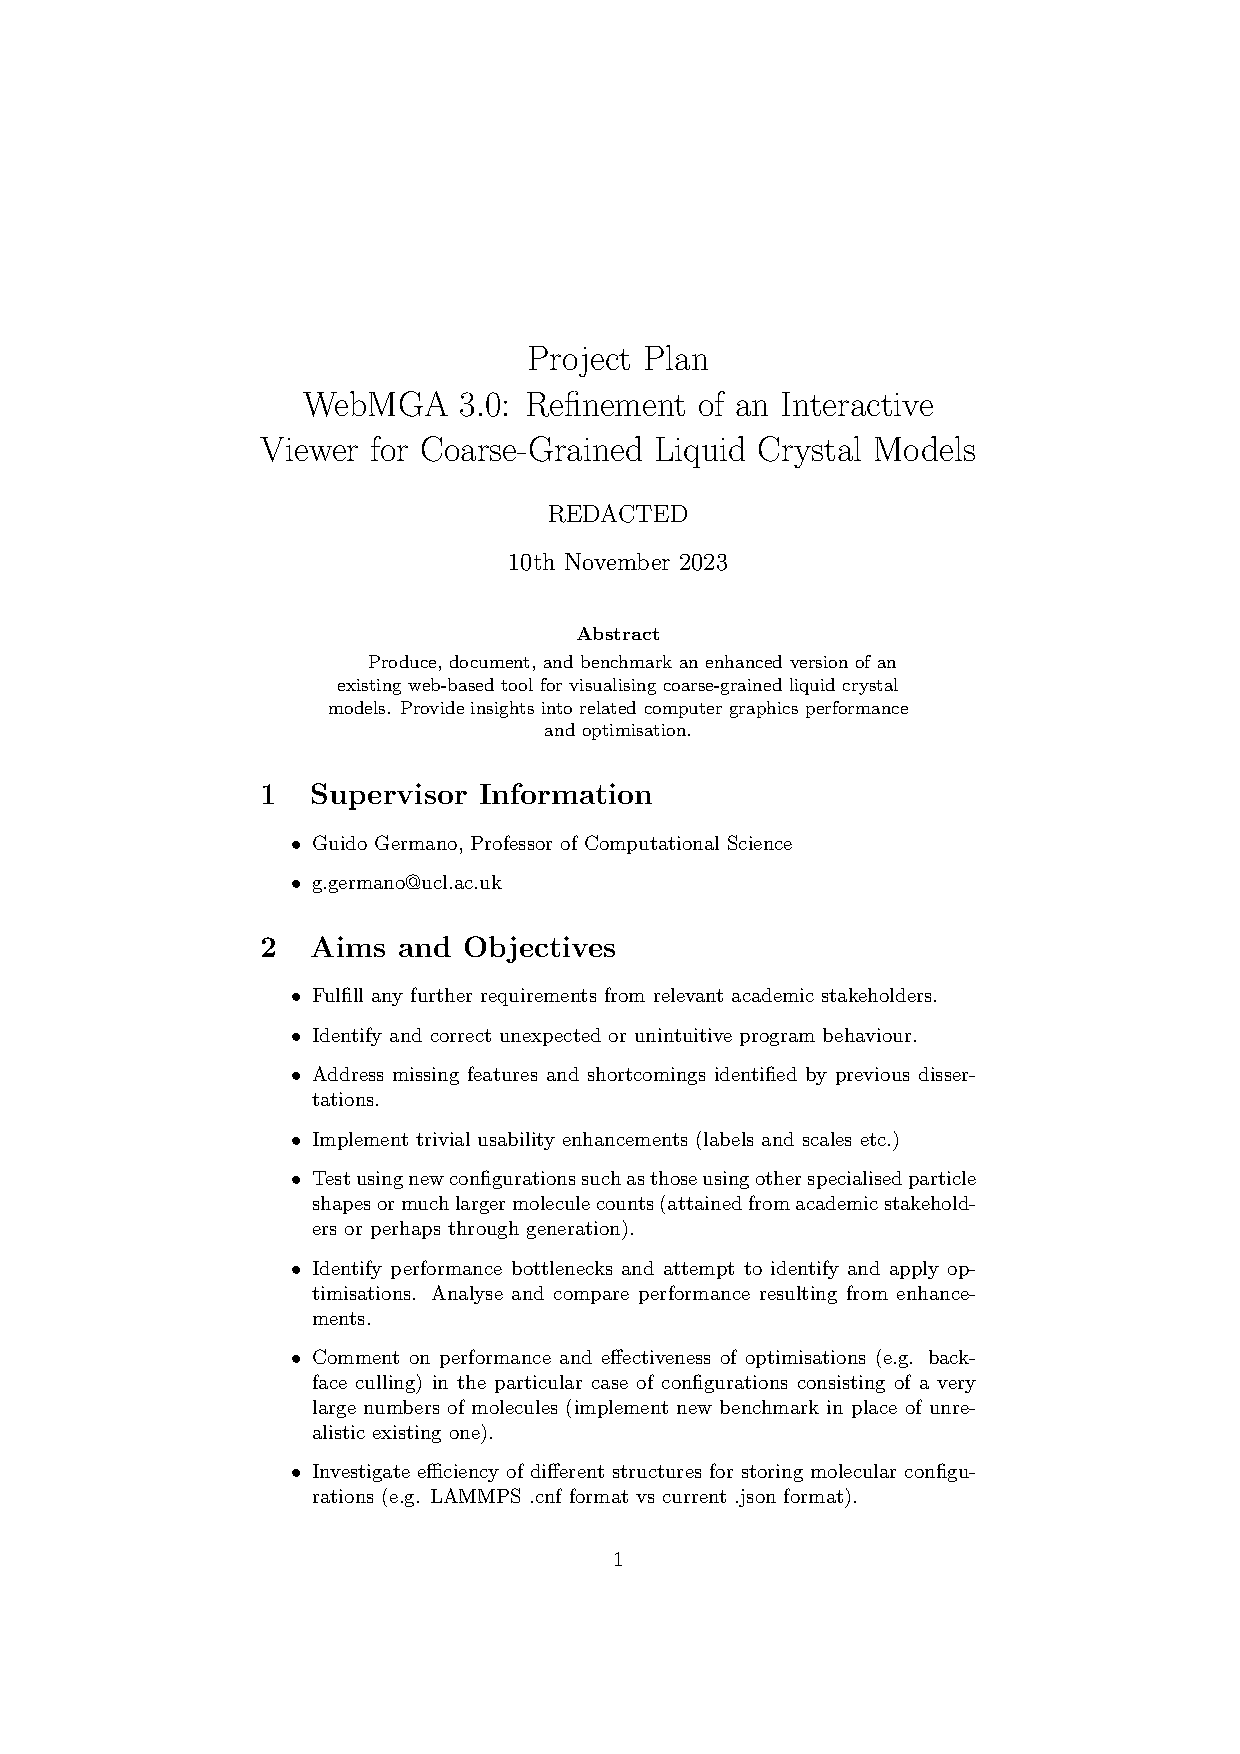
\includepdf[pages=-]{assets/progress_reports/proposal.pdf}

\section{Interim Report}
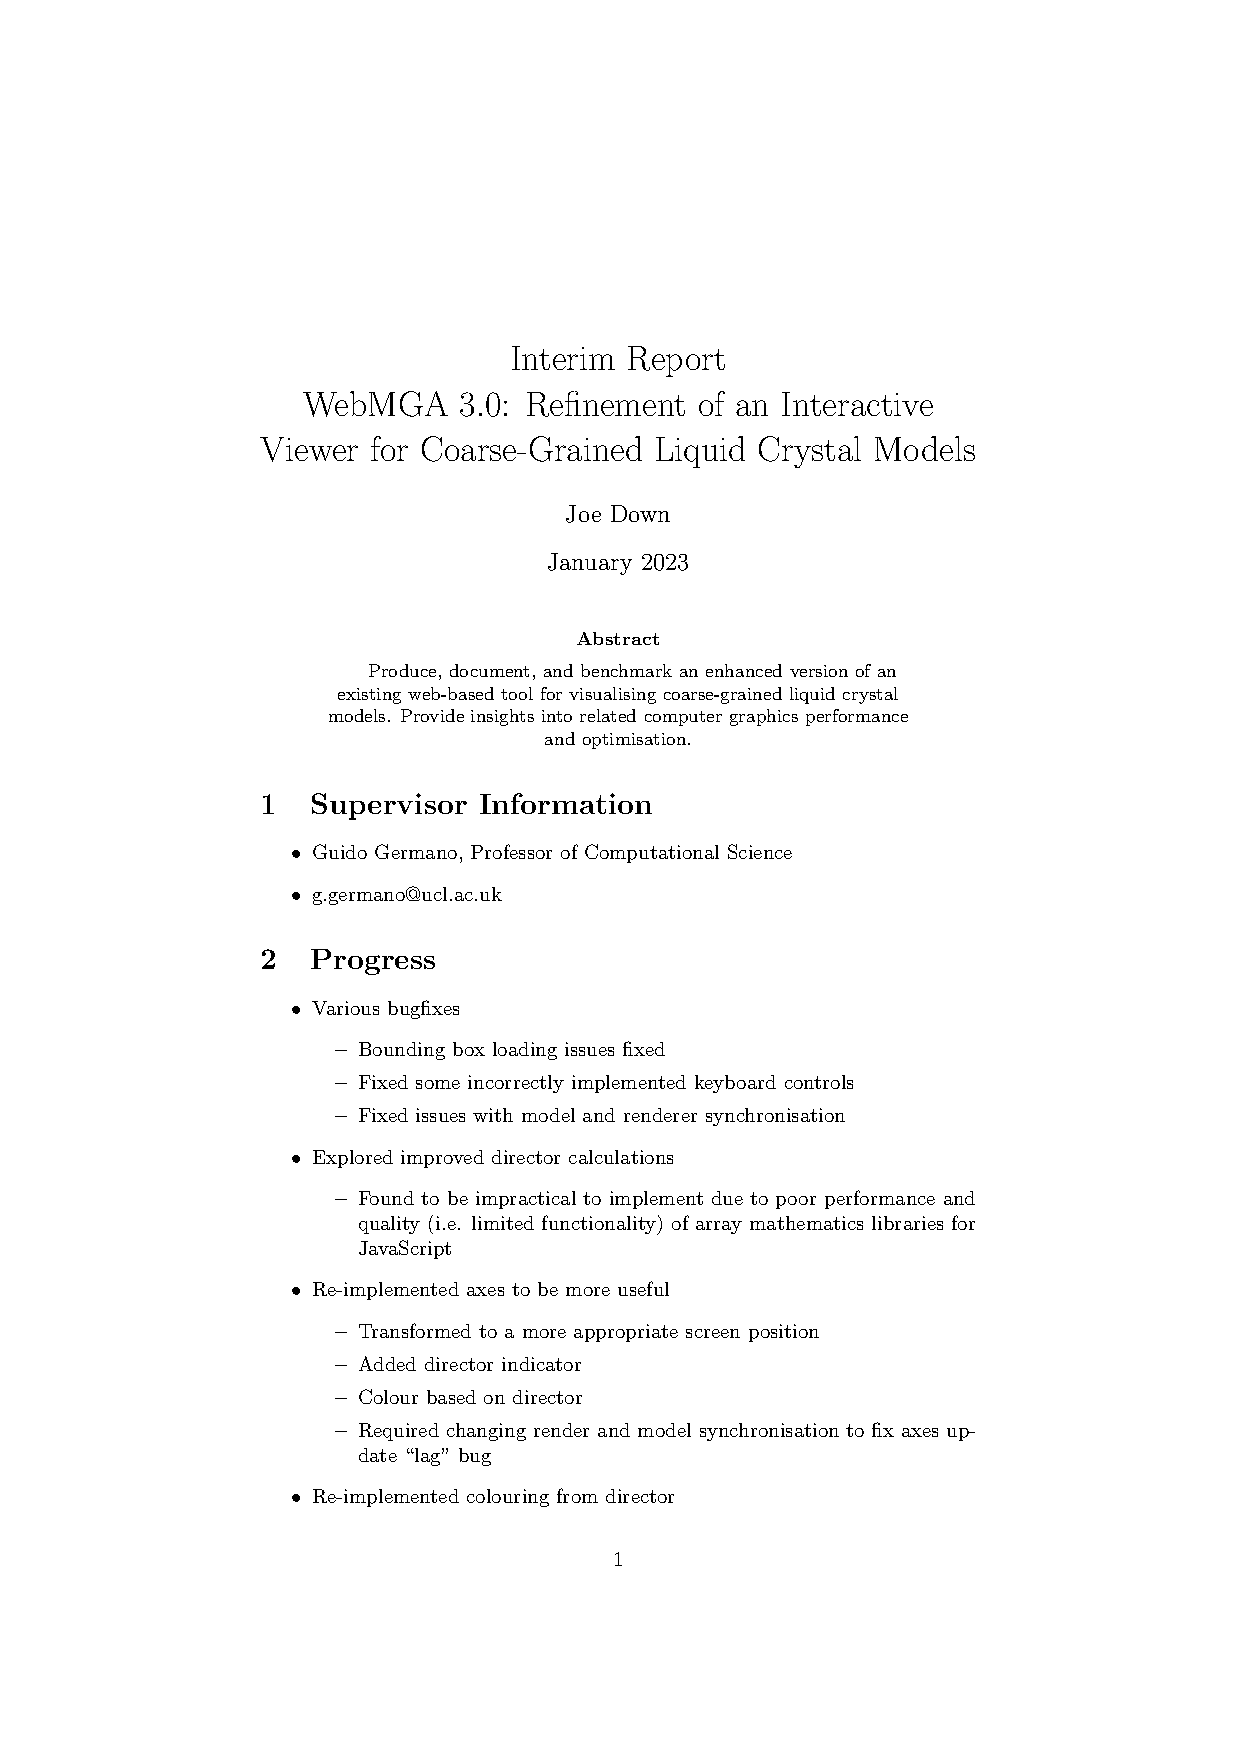
\includepdf[pages=-]{assets/progress_reports/interim.pdf}


\end{document}
